\documentclass[12pt,a4paper,pdftex]{article}

% Sprache
\usepackage[ngerman]{babel}
\usepackage[utf8]{inputenc}

\usepackage{graphicx}

% Page layout
\usepackage{geometry}
\geometry{a4paper,lmargin={2.5cm}, rmargin={2.5cm}, tmargin={2cm}, bmargin={2.5cm}}

% Figure and Caption layout
\usepackage[bf]{caption}
\usepackage{subcaption}
\usepackage{wrapfig}
\usepackage{setspace}

% Befehle zur Textauszeichnung (hervorheben, unterstreichen ect.)
\usepackage{color,soul}
\usepackage{xcolor} % bunter Text

% Zitier-Style für Bücher und URL
\usepackage[numbers]{natbib}
\usepackage[breaklinks=true,bookmarks=true,bookmarksopen=true,colorlinks=true,citecolor=black,linkcolor=black,urlcolor=gray,pdfpagemode=UseNone,pdfstartview=FitH]{hyperref}


\usepackage{float}
\usepackage{gensymb}
\usepackage{siunitx}
\usepackage{tabularx}
\usepackage{amsmath}

% für chemische zeichen
\usepackage[version=4]{mhchem}

% for commenting a whole section
\usepackage{verbatim}

\usepackage{pgfgantt}
\usepackage{afterpage}

% Index
\usepackage{imakeidx}
\makeindex[intoc, columnseprule]
\newcommand{\indextitle}{\section{Index}}

% Bilder importieren
\usepackage{epstopdf}
\epstopdfDeclareGraphicsRule{.pdf}{png}{.png}{convert #1 \OutputFile}
\DeclareGraphicsExtensions{.png,.pdf}

% Bildernummerierung fuer jedes kapitel
\usepackage{chngcntr}
\counterwithin{figure}{section}

% ich hab keine ahnung was die tun und wir brauchen sie auch nicht
%\newcommand{\command}[1]{\texttt{#1}}
%\newcommand{\fileextension}[1]{\texttt{#1}}

% plus minus zeichen
\newcommand{\rpm}{\raisebox{.2ex}{$\scriptstyle\pm$} }

% kapitel title auf deutsch
\renewcommand{\bibsection}{\section{Literaturverzeichnis}}



%%%%%%%%%%%%%%%%%%%%%%%%%%%%%%%%%%%%%%%%%%%%%%%%%%%%%%%%%%%%%

\begin{document}
\setlength{\parindent}{0pt}

%%%%%%%%%%%%%%%%%%%%%%%%%%%%%%%%%%%%%%%%%%%%%%%%%%%%%%%%%%%%%
% Titelseite
%%%%%%%%%%%%%%%%%%%%%%%%%%%%%%%%%%%%%%%%%%%%%%%%%%%%%%%%%%%%%

\begin{titlepage}
 \begin{center}
        \vspace*{1cm}
        \LARGE
        \textbf{Kurzes Lehrbuch der Neuroanatomie des Säugers}
        \vspace{2cm}
        
        \Large
        Praktikumsprotokoll des Mastermoduls Neuroanatomie
        \vspace{4cm}
        
        \large
        vorgelegt von \\ Jacqueline Göbl, Julia Grüb, Marta Provenzano und Laura Seidler % Author name
        \vfill
        \large     
        T\"ubingen, \today
    \end{center}
    \newpage
        \thispagestyle{empty}
        \mbox{}
        \newpage
\end{titlepage}


\thispagestyle{empty}
\mbox{}

%%%%%%%%%%%%%%%%%%%%%%%%%%%%%%%%%%%%%%%%%%%%%%%%%%%%%%%%%%%%%% Inhaltsverzeichnis und Abbildungsverzeichnis
%%%%%%%%%%%%%%%%%%%%%%%%%%%%%%%%%%%%%%%%%%%%%%%%%%%%%%%%%%%%%

\tableofcontents
\newpage
\listoffigures

%%%%%%%%%%%%%%%%%%%%%%%%%%%%%%%%%%%%%%%%%%%%%%%%%%%%%%%%%%%%%
% Textbeginn
%%%%%%%%%%%%%%%%%%%%%%%%%%%%%%%%%%%%%%%%%%%%%%%%%%%%%%%%%%%%%

\newpage
\section{Einleitung}
%%%%%%%%%%%%%%%%%%%%%%%%%%%%%%%%%%%%%%%%%%%%%%%%%%%%%%%%%%%%%

\newpage
\section{Material und Methoden}
%%%%%%%%%%%%%%%%%%%%%%%%%%%%%%%%%%%%%%%%%%%%%%%%%%%%%%%%%%%%%

Computerprogramm am Aufnahmecomputer der Bilder:
Axio Vision (AxioVs40 4.8.2.0, Copyright 2006-2010, Carl zeiss MicroImaging GmBH)


\begin{itemize}
    \item Schafhirn - die Präperationsanleitungen hat auch Jacqui
    \item Perfusion der Ratte - hat auch Jacqui
    \item Färbungen (Nissl, Faser, Immunohistochemie)
    \item Auswertung am Mikroskop - Jacqui hat die genauen Angaben des Programms welches wir für die Mikroskopaufnahmen benutzt wurde
\end{itemize}


%%%%%%%%%%%%%%%%%%%%%%%%%%%%%%%%%%%%%%%%%%%%%%%%%%%%%%%%%%%%%
%%%%%%%%%%%%%%%%%%%%%%%%%%%%%%%%%%%%%%%%%%%%%%%%%%%%%%%%%%%%%

%_____________________JULES_ABSCHNITT________________________

\newpage
\section{Entstehung des Gehirns}
%%%%%%%%%%%%%%%%%%%%%%%%%%%%%%%%%%%%%%%%%%%%%%%%%%%%%%%%%%%%%

\subsection{Neurulation}
\label{subsec:Neurulation} \index{Neurulation}
%%%%%%%%%%%%%%%%%%%%%%%%%%%%%%%%%%%%%%%%%%%%%%%%%%%%%%%

\begin{minipage}[b]{0.68\textwidth}
Der Embryo entwickelt drei Keimblätter: Endoderm, Mesoderm und Ektoderm. Aus diesen werden in späteren Entwicklungsschritten unterschiedliche Gewebe und Organe des adulten Individuums entstehen. Aus dem Mesoderm entstehen Skelett-, Muskel- und Bindegewebe, aus dem Endoderm Verdauungs-, Atem- und Urogenitaltrakt. Aus dem Ektoderm entstehen später die Haut und das Nervensystem \textsuperscript{\cite[1]{crossman2014neuroanatomy}}. Die Entwicklung des Nervensystems beginnt mit der Neuralinduktion. Durch einen Anreiz des Mesoderms und der Chorda dorsalis bildet das darüber liegende Ektoderm das sogenannte Neuroektoderm aus. Das Neuroektoderm bildet dann die Neuralplatte aus (Abb.~\ref{fig:neurulation}). Im Laufe der Neurulation senkt sich diese in Richtung des Mesoderms ab und bildet so die Neuralrinne. Die angrenzenden Strukturen werden dadurch leicht erhöht und bilden die Neuralfalten. Durch weiteres Absinken und Abschnüren entsteht aus der Neuralrinne schließlich das Neuralrohr, aus den Neuralfalten die Neuralleisten. Aus der \textbf{Neuralleiste} werden im späteren Verlauf die Strukturen des peripheren Nervensystems entstehen. Aus dem \textbf{Neuralrohr} entwickelt sich das zentrale Nervensystem. Im Bereich des Kopfes bildet es das Gehirn aus, im hinteren Rumpfabschnitt das Rückenmark. Aus dem Hohlraum, den das Neuralrohr umschließt, entsteht das Ventrikelsystem\index{Ventrikelsystem} \textsuperscript{\cite[1]{trepel2011neuroanatomie}}.
\end{minipage} \hspace{0.1cm}
\begin{minipage}[b]{0.3\textwidth}
\begin{figure}[H]
    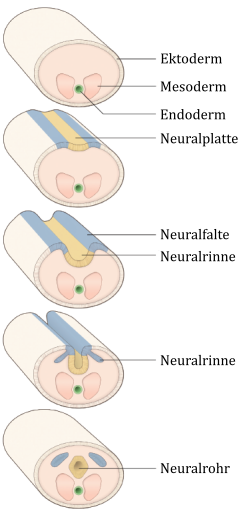
\includegraphics[width=\textwidth]{pictures/Bilder_Jule/Andere/Neurulation_crossm1.png}
    \caption[Neurulation]{\textbf{\newline Neurulation} \textsuperscript{\cite[1]{crossman2014neuroanatomy}}}
    \label{fig:neurulation}
    \end{figure}    
\end{minipage} 

\subsection{Cephalisation}
\label{subsec:Cephalisation} \index{Cephalisation}
%%%%%%%%%%%%%%%%%%%%%%%%%%%%%%%%%%%%%%%%%%%%%%%%%%%%%%%
Zentrales und Peripheres Nervensystem der Wirbeltiere werden von unterschiedlichen ontogenetischen Strukturen gebildet. Das Periphere Nervensystem (PNS) wird aus Zellen der mesodermalen Neuralleiste gebildet. Im Gegensatz dazu wird das Zentrale Nervensystem (ZNS), das sowohl Gehirn als auch Rückenmark umfasst, von den Zellen des Neuralrohrs gebildet. Somit ist das ZNS ektodermalen Ursprungs. \\

\begin{figure}[H]
\centering
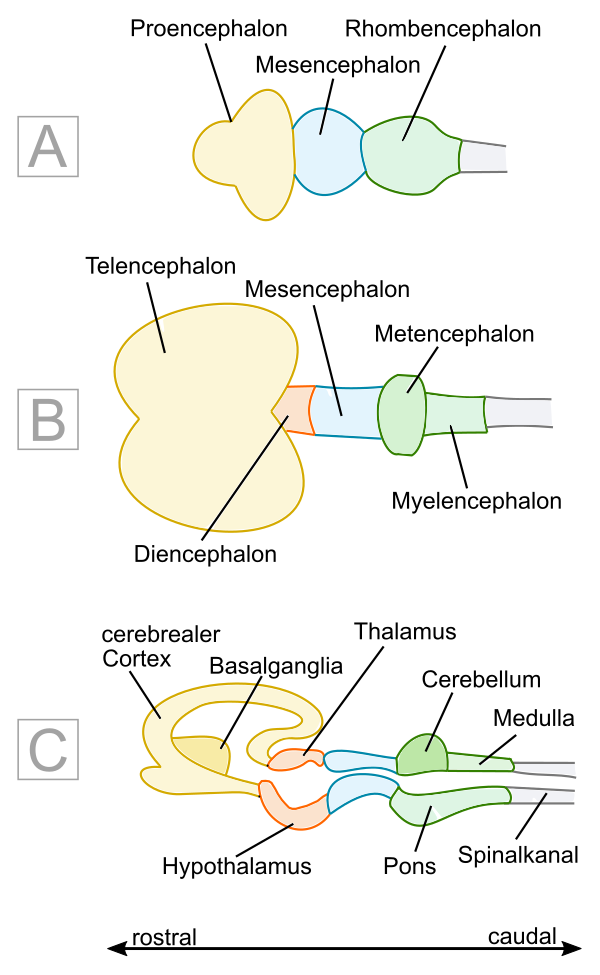
\includegraphics[width=0.5\textwidth]{pictures/Bilder_Jule/Andere/cephalisation.png}
\caption[Grundgliederung des Säugerhirns]{\textbf{Grundgliederung des Säugerhirns.} \textbf{A}:~primäre Hirnbläschen (3), \textbf{B}:~sekundäre Hirnbläschen (5), \textbf{C}:~Grundgliederung und Ventrikelsystem. Nach Baer \textsuperscript{\cite[7]{neurowissenschaften_baer}}.}
\label{fig:cephalisation}
\end{figure}

\noindent Im Laufe der Cephalisation bildet das frühe Neuralrohr rostral drei Schwellungen aus. Diese dehnen sich zunehmend aus und bilden die primären Hirnbläschen: Vorderhirn (Proencephalon)\index{Proencephalon}, Mittelhirn (Mesencephalon) und Rautenhirn (Rhombencephalon)\index{Rhombencephalon} (Abb.~\ref{fig:cephalisation}~A). Diese entwickeln sich im Laufe der Gehirnentwicklung zu den fünf sekundären Hirnbläschen: Das Proencephalon bildet zwei laterale Fortsätze aus, die cerebralen Vesikel,  die später die Hemisphären des cerebralen Cortex bilden werden. Zusammen mit dem rostralen Vorderhirn bilden sie das Endhirn (\textbf{Telencephalon})\index{Telencephalon}. Der caudale Teil des Vorderhirns bildet das Zwischenhirn (\textbf{Diencephalon})\index{Diencephalon} aus dem Thalamus und Hypothalamus gebildet werden. Das Mittelhirn (\textbf{Mesencephalon})\index{Mesencephalon} formt vier Schwellungen, die zum inferioren und superioren Colliculus heranwachsen. Das Rautenhirn gliedert sich in Hinterhirn (\textbf{Metencephalon})\index{Metencephalon} und Nachhirn (\textbf{Myelencephalon})\index{Myelencephalon} auf, die später Pons und Cerebellum (Metencephalon), beziehungsweise die Medulla (Myelencephalon) bilden (Abb.~\ref{fig:cephalisation}~C). Zusammengefasst ist das Vertebratengehirn am Ende der Cephalisation in vier Teilbereiche gegliedert; Das Telencephalon, Diencephalon, Mesencephalon und das Rhombencephalon, das Met- und Myelencephalon zusammenfasst (Abb.~\ref{fig:cephalisation}~B) \textsuperscript{\cite[10]{watson2010thebrain}}.

\subsection{Das Ventrikelsystem}
\label{subsec:} \index{Ventrikelsystem}
%%%%%%%%%%%%%%%%%%%%%%%%%%%%%%%%%%%%%%%%%%%%%%%%%%%%%%%

Jedes dieser Hirnvesikel umhüllt dabei einen mit Hirnwasser (\textit{Liquor cerebrospinalis}) gefüllten Hohlraum. Diese miteinander in Verbindung stehenden Ventrikel bilden das Ventrikelsystem (Abb.~\ref{fig:ventrikelsystem}), das auch als innerer Liquorraum  bezeichnet wird. Es besteht aus vier Ventrikeln: Zwei laterale Ventrikel, auch Seitenventrikel genannt, befinden sich im Telencephalon. Sie verlaufen entlang des Hippocampus, der ihre mediale Wand bildet. Der dritte Ventrikel befindet sich im Diencephalon. Im Gegensatz zu den lang gezogenen lateralen Ventrikeln befindet sich der dritte Ventrikel spaltförmig in der Midsagittalebene des Gehirns. Das Mesencephalon umgibt das Aquädukt (\textit{Aqueductus cerebri} oder \textit{Aqueductus mesencephali}). Es liegt unter der Vierhügelplatte und über dem Tegmentum. Der vierte und letzte Ventrikel ist im Rhombencephalon lokalisiert und erstreckt sich oberhalb des Hirnstamm und unterhalb des Cerebellums bis hin zum Rückenmark
\textsuperscript{\cite[2]{watson2010thebrain}}.

\begin{figure}[H]
	\centering
	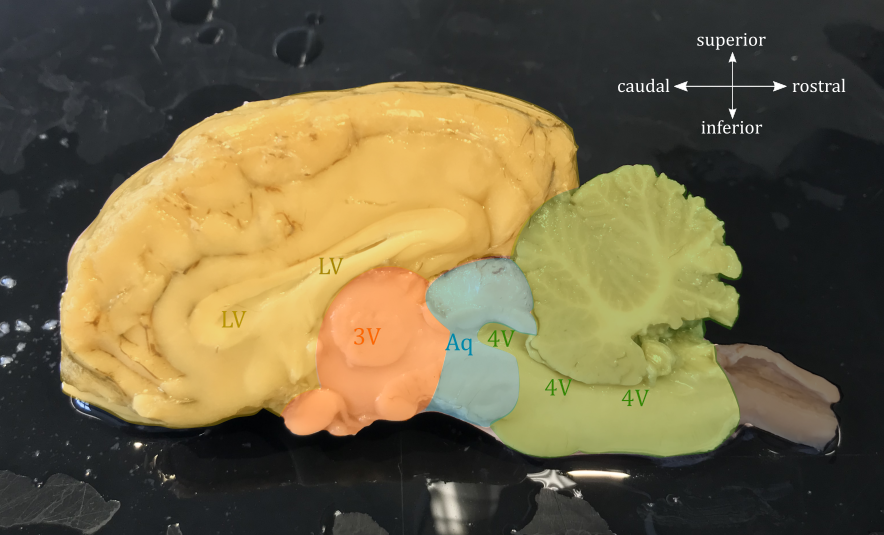
\includegraphics[width=0.8\textwidth]{pictures/Bilder_Jule/Andere/ventrikelsystem.png}
	\caption[Das Ventrikelsystem]{\textbf{Das Ventrikelsystem.} Das Ventrikelsystem im Midsagittalschnitt des Schafhirns. Das Telencephalon und der laterale Ventrikel (LV) sind gelb, Diencephalon und dritter Ventrikel (3V) orange, Mesencephalon und Aquädukt (Aq) blau und Rhombencephalon, sowie vierter Ventrikel (4V) rot gefärbt.}
	\label{fig:ventrikelsystem}
\end{figure}

\noindent Innerhalb der Ventrikel sind die \textbf{Plexus choroidei} \index{Choroid plexus} lokalisiert. Sie bestehen aus arterovenösen Gefäßästen, die von einem speziellen Epithel, dem Plexusepithel, überdeckt sind. Der Plexus choroideus produziert den Liquor \index{Liquor cerebrospinalis}, der das Gehirn umgibt. Dabei werden beim Menschen täglich, vor allem vom Plexus der lateralen Ventrikel, etwa 500~ml Liquor produziert. Diese klare Flüssigkeit, die nur wenige Zellen, hauptsächlich Leukozyten, und einen geringen Anteil an Eiweiß und Glucose enthält, dient als Druck- und Stoßdämpfer des Gehirns. Auch hält er das extrazelluläre Milieu konstant. Durch den Liquorfluss können zudem potentiell schädliche Metabolite entfernt werden \textsuperscript{\cite[10]{trepel2011neuroanatomie}}. 

\section{Räumliche Übersicht}
\label{sec:raeumliche_uebersicht}
%%%%%%%%%%%%%%%%%%%%%%%%%%%%%%%%%%%%%%%%%%%%%%%%%%%%%%%%%%%
%%%%%%%%%%%%%%%%%%%%%%%%%%%%%%%%%%%%%%%%%%%%%%%%%%%%%%%%%%%

Das \textbf{Telencephalon}\index{Telencephalon} (gelb) ist das rostralste Hirnareal (Abb.~\ref{fig:schaf_midsagittal}). In ihm verlaufen die lateralen Ventrikel (LV: Abb.~\ref{fig:schaf_midsagittal}~A, \ref{fig:schaf_lateral_sagittal}~B-L, \ref{fig:coronal_schaf}~C-H). Das Telencephalon beinhaltet die Großhirnrinde (Cx), die aus zwei Großhirnhemisphären besteht. Über die Fasern des Corpus callosum\index{Corpus callosum} (cc) stehen die beiden Hemisphären miteinander in Verbindung (Abb.~\ref{fig:schaf_midsagittal}~A, \ref{fig:schaf_lateral_sagittal}~H, \ref{fig:coronal_schaf}~C-G). Zudem kann die Großhirnrinde in Neo-, Archi- und Paleocortex\index{Paleocortex} unterteilt werden. Am rostralen Ende des Gehirns befindet sich der Riechkolben (Bulbus olfactorius, OB)\index{Bulbus olfactorius}, der Teil des Riechhirns und somit des Paleocortex ist (Abb.~\ref{fig:schaf_midsagittal}~A, \ref{fig:schaf_lateral_sagittal}~I-J,
\ref{fig:coronal_schaf}~A-C). Der Neocortex\index{Neocortex} (NCx) ist eher superior-lateral gelegen. Er wird von der Fissura rhinalis (RF) räumlich vom eher inferior gelegenen Archicortex\index{Archicortex} (ACx) getrennt (Abb.~\ref{fig:coronal_schaf}~A-H). Ein Teilgebiet des Archicortex ist der cinguläre Cortex\index{cingulärer Cortex} (CCx). Dieser erstreckt sich von rostral nach caudal über dem Corpus callosum, dem Hippocampus und dem lateralen Ventrikel (Abb.~\ref{fig:schaf_lateral_sagittal}~K-L). Auch der Hippocampus\index{Hippocampus} (Hi) gehört zum Archicortex. Er ist medial im Telencephalon gelegen und umgibt c-förmig den Thalamus (Th) des Diencephalons (Abb.~\ref{fig:coronal_schaf}~G). Die Fimbria\index{Fimbria} (fi), eine schmale Faserstruktur, bildet am medialen Ende des Hippocampus den Beginn des Fornix\index{Fornix} (Abb.~\ref{fig:coronal_schaf}~G). Über die Fasern des Fornix (f) ist der Hippocampus mit dem inferior gelegenen Mammillarkörper (MB) verbunden (Abb.~\ref{fig:schaf_midsagittal}~B). Auch Teile der Basalganglia\index{Basalganglia} sind im Telencephalon lokalisiert. Dazu gehören das Caudoputamen und der Nucleus caudatus. Der Ncl. caudatus\index{Nucleus caudatus} (Cu) ist medial im Telencephalon unter dem cerebralen Cortex gelegen. Er bildet einen Teil der lateralen Wand des lateralen Ventrikels (Abb.~\ref{fig:schaf_midsagittal}~C, \ref{fig:schaf_lateral_sagittal}~J-L, \ref{fig:coronal_schaf}~E-F). Das Caudoputamen\index{Putamen} (CPu) liegt lateral, inferior und leicht rostral des Ncl. caudatus (\ref{fig:schaf_lateral_sagittal}~I, Abb.~\ref{fig:coronal_schaf}~D-F). Durch die Capsula externa (ec) sind beide Strukturen räumlich voneinander getrennt (Abb.\ref{fig:coronal_schaf}~E).

\noindent Das \textbf{Diencephalon}\index{Diencephalon} (orange) schließt sich caudal an das Telencephalon an und wird im superioren Bereich von diesem verdeckt. Es umschließt den dritten Ventrikel (3V), der mittig einen flachen Hohlraum im Gehirn bildet (Abb.~\ref{fig:schaf_midsagittal}~A,B, \ref{fig:coronal_schaf}~F-H). Von superior nach inferior kann das Diencephalon in Epithalamus, Thalamus, Subthalamus und Hypothalamus gegliedert werden. Die Epiphyse\index{Epiphyse} (Epi), als superiorster Teil des Zwischenhirns, gehört zum Epithalamus. Sie liegt caudal im Diencephalon, rostral der Vierhügelplatte, unter dem cerebralen Cortex (Abb.~\ref{fig:schaf_midsagittal}~D). Der Thalamus\index{Thalamus} (Th) bildet einen Teil der Wand des dritten Ventrikels. Er wird vom Hippocampus umschlungen (Abb.~\ref{fig:coronal_schaf}~G). Der Corpus geniculatum laterale\index{Corpus geniculatum laterale, LGN} (LGN), eine Station der Sehbahn, ist superior im Thalamus gelegen. Ebenfalls Teil der Sehnbahn ist das Chiasma opticum\index{Chiasma opticum} (ox) an dem sich die optischen Trakte kreuzen. Diese Faserkreuzung befindet sich rostral des Thalamus und ist inferior an das Diencephalon angelagert (Abb.~\ref{fig:schaf_midsagittal}~A, \ref{fig:schaf_lateral_sagittal}J-L). Inferior des Thalamus, unter dem Subthalamus, liegt der Hypothalamus\index{Hypothalamus}. Er bildet die untere Wand des dritten Ventrikels. Ein Teilgebiet des Hypothalamus ist der Mammillarkörper\index{Mammillarkörper} (MB). Er liegt am inferioren Ende des Gehirns, caudal des optischen Chiasmas (Abb.~\ref{fig:schaf_midsagittal}~A,B).

\noindent Weiter caudal liegt das \textbf{Mesencephalon}\index{Mesencephalon} (blau). Es umschließt das Aqueductus mesencephali (Aq), das zwischen drittem und viertem Ventrikel liegt (Abb.~\ref{fig:schaf_midsagittal}~A,B). Superior ist das Tectum gelegen. Es besteht aus der Vierhügelplatte\index{Vierhügelplatte}, die aus den superioren\index{Colliculus superior, SC} (SC) und inferioren Colliculi\index{Colliculus inferior, IC} (IC) aufgebaut ist. Die paarigen Colliculi superiores liegen rostral und superior der ebenfalls paarigen Colliculi inferiores (Abb.~\ref{fig:schaf_midsagittal}~D), \ref{fig:schaf_lateral_sagittal}~K-L, \ref{fig:coronal_schaf}~H-I). Unter dem Tectum liegt das Tegmentum mesencephali\index{Tegmentum !Tegmentum mesencephali} (Teg). Es liegt zwischen dem Mammillarkörper und dem Rhombencephalon (Abb.~\ref{fig:schaf_midsagittal}~A).

\noindent Das Rhombencephalon\index{Rhombencephalon} (grün) ist in Met- und Myelencephalon unterteilt. Im inferioren \textbf{Metencephalon}\index{Metencephalon} liegt der Pons\index{Pons} (Pn: Abb.~\ref{fig:schaf_midsagittal}~A, \ref{fig:coronal_schaf}~I-J). Im superioren Bereich des Metencephalons, über dem Pons, befindet sich das Cerebellum\index{Cerebellum} (Cb: Abb.\ref{fig:schaf_midsagittal}~A). Es ist über die Fasern der Kleinhirnstiele oder Kleinhirn-Pedunkel\index{Kleinhirnpedunkel} (cp) mit Mesencephalon, Pons und Medulla verbunden (Abb.~\ref{fig:schaf_lateral_sagittal}~D-E, \ref{fig:coronal_schaf}~I). Die Kleinhirnsegel oder Veli\index{Velum} (ve) bilden das Dach des vierten Ventrikels (4V), der sich zwischen Pons und Cerebellum in rostro-caudaler Richtung erstreckt (Abb.~\ref{fig:schaf_midsagittal}~A, \ref{fig:coronal_schaf}~J). Das \textbf{Myelencephalon}\index{Myelencephalon} besteht aus der Medulla\index{Medulla oblongata} (Med), die caudal an den Pons angrenzt. Weiter caudal geht die Medulla in das Rückenmark\index{Rückenmark} (CS) über. Dabei geht der offene vierte Ventrikel, der superior entlang der Medulla verläuft, in den geschlossenen Zentralkanal des Rückenmarks über (Abb.~\ref{fig:schaf_midsagittal}~A,E, \ref{fig:coronal_schaf}~L).



\newpage
\subsection{Midsagittalschnitt}
\label{subsec:midsagittal}
%%%%%%%%%%%%%%%%%%%%%%%%%%%%%%%%%%%%%%%%%%%%%%%%%%%%%%%

\begin{figure}[H]
\centering
\begin{minipage}[b]{.8\textwidth}
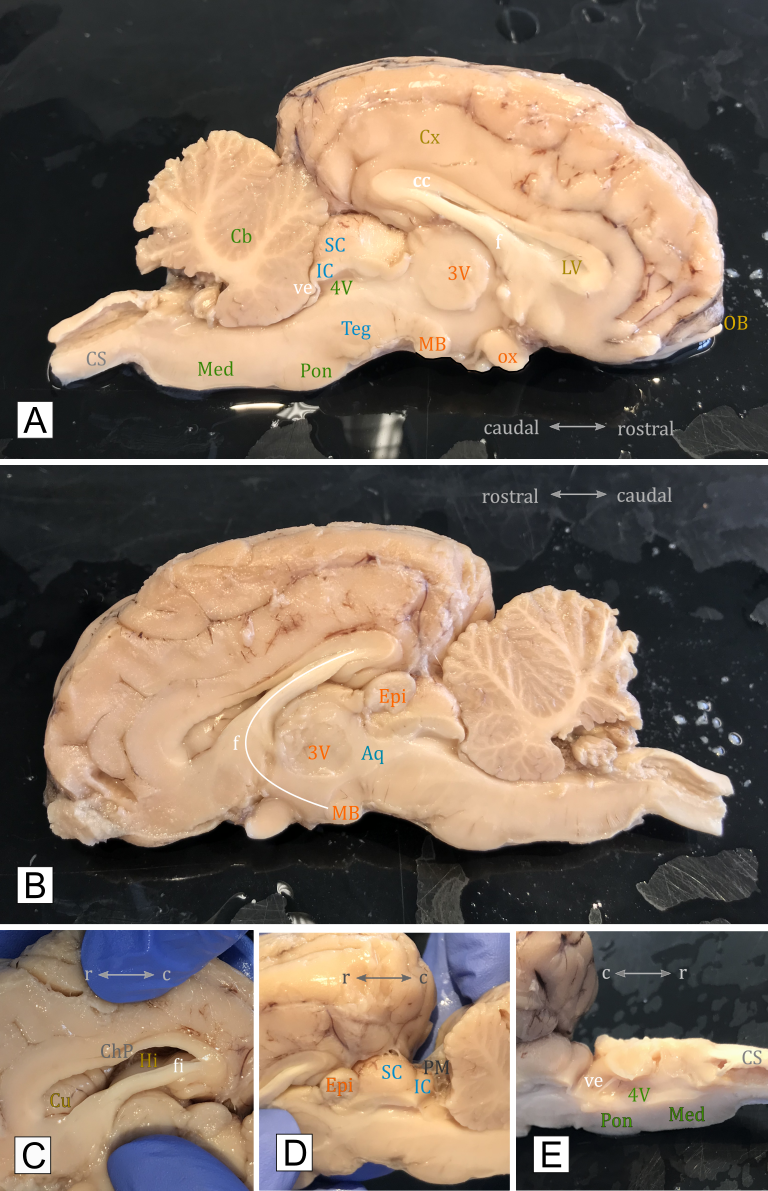
\includegraphics[width=\textwidth]{pictures/Bilder_Jule/Schaf/mittsagittal/schaf_mittsagittal_alle.png}
\end{minipage}
\caption[Midsagittalschnitt Schaf]{\textbf{Midsagittalschnitt Schaf. A}: linke Hemisphäre, \textbf{B}: rechte Hemisphäre, \textbf{C}: lateraler Ventrikel, \textbf{D}: Vierhügelplatte, \textbf{E}: Rhombencephalon ohne Cerebellum. Dabei ist in allen Bildern superior oben und inferior unten dargestellt. Bereiche, die dem Telencephalons zuzuordnen sind, sind gelb beschriftet, Bereiche des Diencephalons orange, des Mesencephalons blau und des Rhombencephalons grün. Fasern, bzw. Nerven sind mittels weißer Beschriftung gekennzeichnet.}
\label{fig:schaf_midsagittal}
\end{figure}


\newpage
\subsection{Laterale Sagittalschnitte}
\label{subsec:lateral_sagittal}
%%%%%%%%%%%%%%%%%%%%%%%%%%%%%%%%%%%%%%%%%%%%%%%%%%%%%%%

\begin{figure}[H]
    \centering
    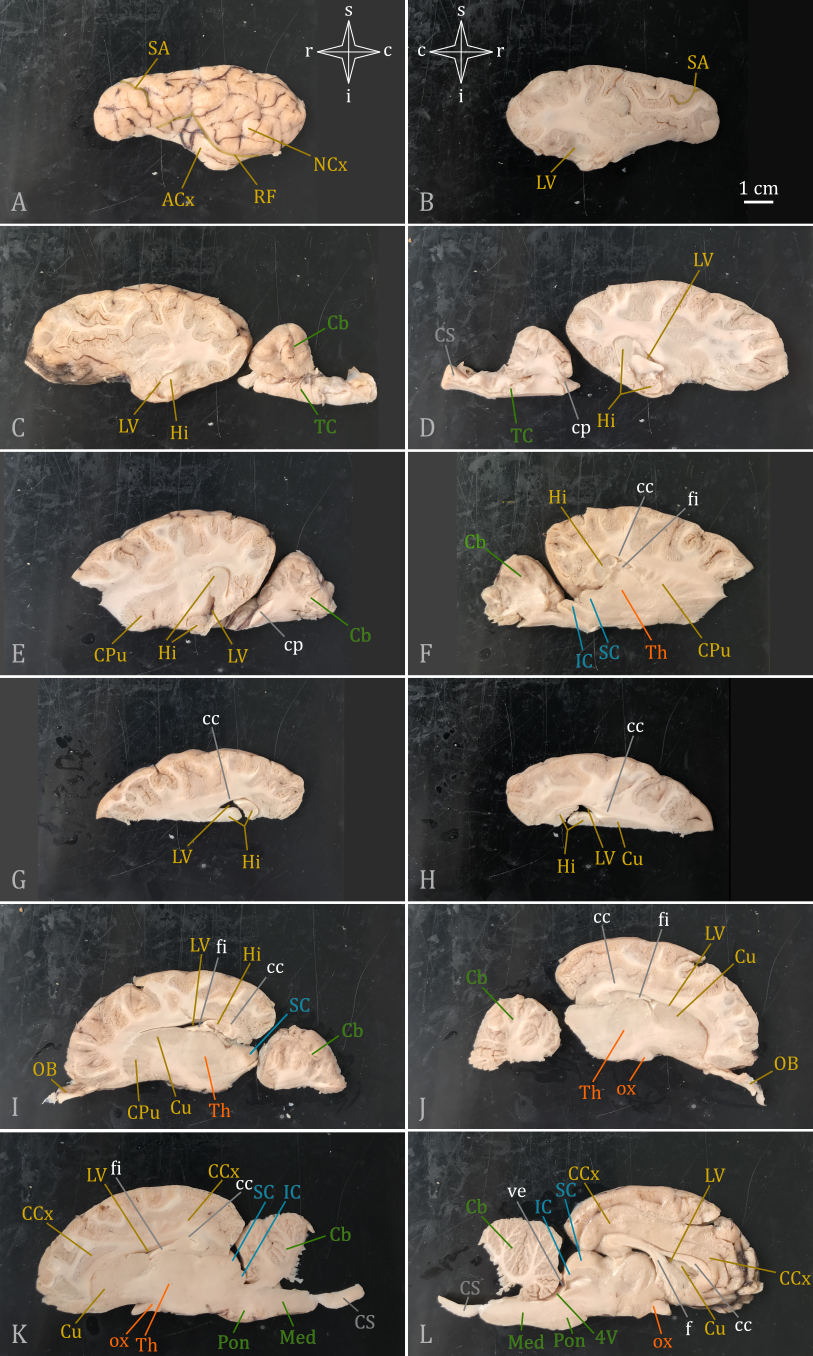
\includegraphics[width=0.8\textwidth]{pictures/Bilder_Jule/Schaf/lateral_sagittal/schaf_lateral_sagittal.png}
    \caption[Laterale Sagittalschnitte Schaf]{\textbf{Laterale Sagittalschnitte Schaf.} Die Schnitte sind von lateral (oben) nach medial (unten) angeordnet. Bereiche des Telencephalons sind gelb gekennzeichnet, Bereiche des Diencephalons orange, des Mesencephalons blau und des Rhombencephalons grün.}
    \label{fig:schaf_lateral_sagittal}
\end{figure}


\newpage
\subsection{Coronalschnitte}
\label{subsec:coronal}
%%%%%%%%%%%%%%%%%%%%%%%%%%%%%%%%%%%%%%%%%%%%%%%%%%%%%%%

\begin{figure}[H]
\centering
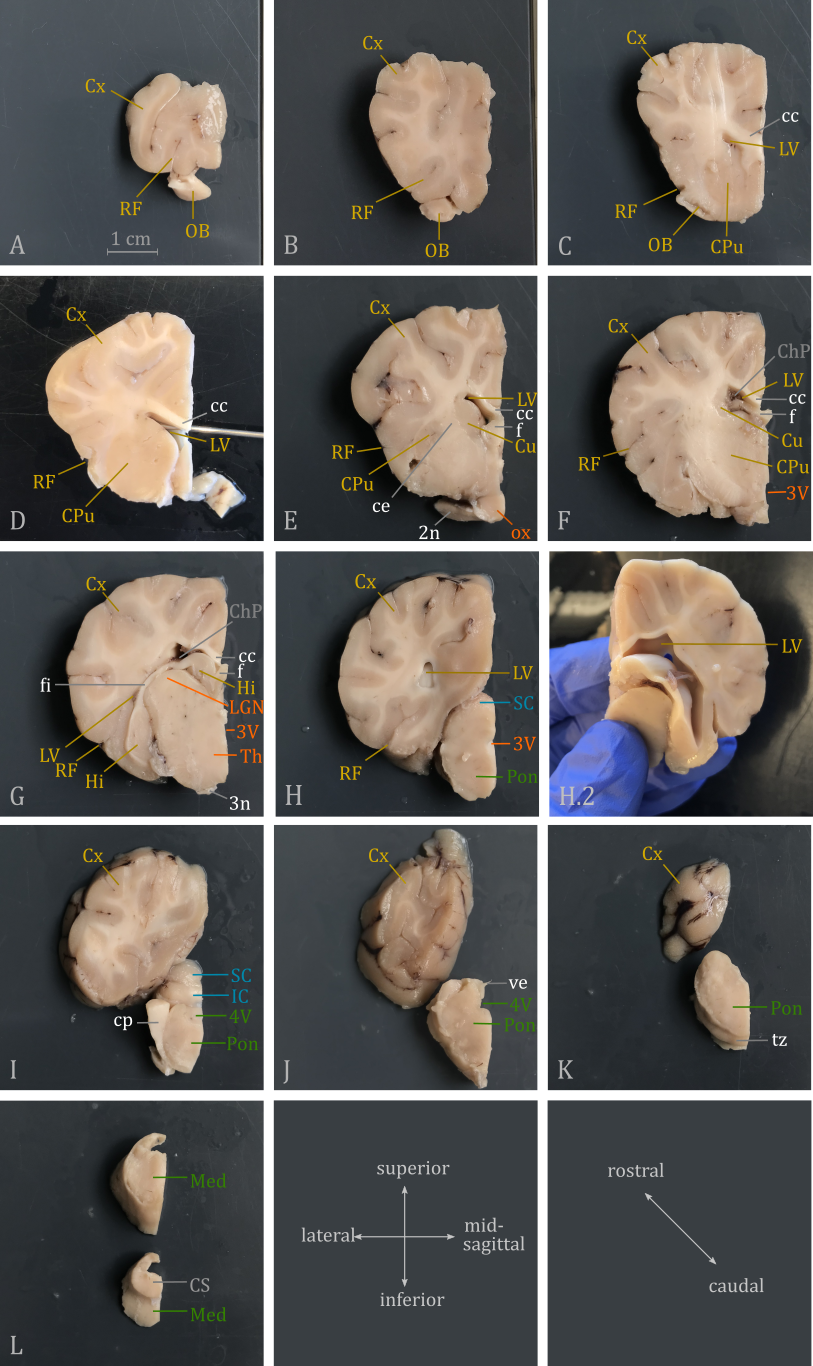
\includegraphics[width=0.8\textwidth]{pictures/Bilder_Jule/Schaf/coronal/coronal_schaf_all.png}
\caption[Coronalschnitte Schaf]{\textbf{Coronalschnitte Schaf.} Von rostral (links oben) nach caudal (rechts unten). Teilgebiete des Telencephalons sind gelb, des Diencephalons orange, des Mesencephalons blau und des Rhombencephalons grün beschriftet. Fasern, bzw. Nerven sind in weiß beschriftet.}
\label{fig:coronal_schaf}
\end{figure}

\subsection{Beschriftung und Kürzel}
%%%%%%%%%%%%%%%%%%%%%%%%%%%%%%%%%%%%%%%%%%%%%%%%%%%%%%%

\begin{comment}
2n \indent - \indent \textit{N. opticus}\\
3V \indent - \indent Dritter Ventrikel\\
3n \indent - \indent \textit{N. oculomotorius}\\
4V \indent - \indent Vierter Ventrikel\\
ACx \indent - \indent Archicortex\\
Aq \indent - \indent Aquädukt, \textit{Aqueductus mesencephali, Aquaeductus cerebri}\\
Cb \indent - \indent Cerebellum, Kleinhirn\\
cc \indent - \indent \textit{Corpus callosum}\\
CCx \indent - \indent cingulärer Cortex, \textit{Gyrus cinguli}\\
ce \indent - \indent \textit{Capsula externa}\\
Chp \indent - \indent \textit{Choroid plexus}\\
cp \indent - \indent Kleinhirn-Pedunkel\\
CPu \indent - \indent Caudoputamen\\
CS\indent - \indent Rückenmark\\
Cu \indent - \indent \textit{Nucleus caudatus}\\
Cx \indent - \indent cerebraler Cortex, \textit{Cortex cerebri}\\
Epi \indent - \indent Epiphyse\\
f \indent - \indent Fornix\\
fi \indent - \indent Fimbria\\
Hip \indent - \indent Hippocampus\\
IC \indent - \indent \textit{Colliculus inferior}\\
LGN \indent - \indent \textit{Corpus geniculatum laterale}\\
LV \indent - \indent lateraler Ventrikel\\
MB \indent - \indent Mammillarkörper\\
Med \indent - \indent Medulla, \textit{Medulla oblongata}\\
NCx \indent - \indent Neocortex\\
OB \indent - \indent \textit{Bulbus olfactorius}\\
ox \indent - \indent optisches Chiasma, \textit{Chiasma opticum}\\
PM \indent - \indent Pia mater\\
Pon \indent - \indent Pons\\
RF \indent - \indent \textit{Fissura rhinalis}\\
SA \indent - \indent \textit{Sulcus ansatus}\\
SC \indent - \indent \textit{Colliculus superior}\\
TC \indent - \indent Hirnstamm, \textit{Truncus cerebri, Truncus encephali}\\
Teg\indent - \indent Tegmentum, \textit{Tegmentum mesencephali}\\
Th \indent - \indent Thalamus\\
tz \indent - \indent Trapezkörper\\
ve \indent - \indent Velum\\
\end{comment}

\begin{table}[H]
\begin{tabular}{llcll}
           & 3V  & \textbf{-} & dritter Ventrikel                                                       & \multicolumn{1}{c}{\textbf{}} \\
\textbf{}  & 3n  & -          & Nervus oculomotorius                                                        & \multicolumn{1}{c}{}          \\
\textbf{}  & 4V  & -          & vierter Ventrikel                                                       & \multicolumn{1}{c}{}          \\
\textbf{A} & ACx & -          & Archicortex                                                             & \multicolumn{1}{c}{}          \\
\textbf{}  & Aq  & -          & Aquädukt, Aqueductus mesencephali, Aquaeductus cerebri                  & \multicolumn{1}{c}{}          \\
\textbf{C} & Cb  & \textbf{-} & Cerebellum, Kleinhirn                                                   & \multicolumn{1}{c}{\textbf{}} \\
           & cc  & \textbf{-} & Corpus callosum                                                         & \multicolumn{1}{c}{\textbf{}} \\
\textbf{}  & CCx & -          & cingulärer Cortex, Gyrus cinguli             & \multicolumn{1}{c}{}          \\
\textbf{}  & ce  & -          & Capsula externa                                                         & \multicolumn{1}{c}{}          \\
\textbf{}  & Chp & -          & Plexus choroideus                                                          & \multicolumn{1}{c}{}          \\
\textbf{}  & cp  & -          & Kleinhirn-Pedunkel                                                      & \multicolumn{1}{c}{}          \\
\textbf{}  & CPu & -          & Caudoputamen                                                            &                               \\
\textbf{}  & CS  & -          & Rückenmark                                                              &                               \\
\textbf{}  & Cu  & -          & Nucleus caudatus                                                        &                               \\
\textbf{}  & Cx  & -          & cerebraler Cortex, Cortex cerebri          &                               \\
\textbf{E} & Epi & -          & Epiphyse                                                                &                               \\
\textbf{F} & f   & -          & Fornix                                                                  &                               \\
\textbf{}  & fi  & -          & Fimbria                                                                 &                               \\
\textbf{H} & Hip & -          & Hippocampus                                                             &                               \\
\textbf{I} & IC  & -          & Colliculus inferior                                                     &                               \\
\textbf{L} & LGN & -          & Corpus geniculatum laterale                                             &                               \\
\textbf{}  & LV  & -          & lateraler Ventrikel                                                     &                               \\
\textbf{M} & MB  & -          & Mammillarkörper                                                         &                               \\
\textbf{}  & Med & -          & Medulla, Medulla oblongata                  &                               \\
\textbf{N} & NCx & -          & Neocortex                                                               &                               \\
\textbf{O} & OB  & -          & Riechkolben, Bulbus olfactorius                                                      &                               \\
\textbf{}  & ox  & -          & optisches Chiasma, Chiasma opticum           &                               \\
\textbf{P} & PM  & -          & Pia mater                                                               &                               \\
\textbf{}  & Pon & -          & Pons                                                                    &                               \\
\textbf{R} & RF  & -          & Fissura rhinalis                                                        &                               \\
\textbf{S} & SA  & -          & Sulcus ansatus                                                          &                               \\
\textbf{}  & SC  & -          & Colliculus superior                                                     &                               \\
\textbf{T} & TC  & -          & Hirnstamm, Truncus cerebri, Truncus encephali &                               \\
\textbf{}  & Teg & -          & Tegmentum, Tegmentum mesencephali           &                               \\
\textbf{}  & Th  & -          & Thalamus                                                                &                               \\
\textbf{}  & tz  & -          & Trapezkörper                                                            &                               \\
\textbf{V} & ve  & -          & Velum                                                                   &                              
\end{tabular}
\end{table}
%%%%%%%%%%%%%%%%%%%%%%%%%%%%%%%%%%%%%%%%%%%%%%%%%%%%%%%%%%%
%%%%%%%%%%%%%%%%%%%%%%%%%%%%%%%%%%%%%%%%%%%%%%%%%%%%%%%%%%%

\section{Allgemeine Übersicht}
%%%%%%%%%%%%%%%%%%%%%%%%%%%%%%%%%%%%%%%%%%%%%%%%%%%%%%%%%%%
%%%%%%%%%%%%%%%%%%%%%%%%%%%%%%%%%%%%%%%%%%%%%%%%%%%%%%%%%%%

\subsection{Telencephalon}
\label{subsec:Telencephalon} \index{Telencephalon}
%%%%%%%%%%%%%%%%%%%%%%%%%%%%%%%%%%%%%%%%%%%%%%%%%%%%%%%%%%%
%%%%%%%%%%%%%%%%%%%%%%%%%%%%%%%%%%%%%%%%%%%%%%%%%%%%%%%%%%%

Das Telencephalon oder das Endhirn ist eines der fünf Hirnareale, in die sich das Gehirn nach der Cephalisation gliedern lässt. Das Telencephalon befindet sich am rostralen Ende des Gehirns und überdeckt bei Säugern teilweise das superiore Diencephalon. Auch Bereiche des Mesencephalons können von ihm verdeckt werden. Generell kann das Telencephalon in corticale Gebiete (Großhirnrinde), Mark (weiße Substanz) und subcortikale Kerngebiete, zu denen die Basalganglia und die Amygdala gehören, unterteilt werden. 

\subsubsection{Großhirnrinde}
\label{subsubsec:Grosshirnrinde}
%%%%%%%%%%%%%%%%%%%%%%%%%%%%%%%%%%%%%%%%%%%%%%%%%%%%%%%%%%%

Der cerebrale Cortex (\textit{Cortex cerebri}) \index{Cortex cerebri} umhüllt das Gehirn und macht bei Säugern den größten Teil der Außenfläche des Gehirns aus. Er besteht aus zwei Hemisphären, die durch einen dicken Faserstrang, den \textit{Corpus callosum} \index{Corpus callosum} oder Balken, miteinander in Verbindung stehen. Im Laufe der Evolution expandierte der cerebrale Cortex der Säuger und verdeckt dadurch jene Strukturen des Endhirns, die innerhalb der Hemisphären liegen. Im Allgemeinen dient die Großhirnrinde der Analyse und Integration sensorischer Information, sowie der Verknüpfung  dieses Inputs mit bereits gespeicherten Informationen und Erfahrungen. Des Weiteren ist der cerebrale Cortex die 'Steuerzentrale' von Verhalten, das weit über simple Reflexe und Reaktionen hinausreicht. Diese analytischen und integrativen Fähigkeiten des Cortex resultieren aus seiner zellulären Organisation sowie der Kommunikation mit den restlichen Strukturen des zentralen Nervensystems \textsuperscript{\cite[7]{watson2010thebrain}}.


\subsubsection*{Faltung der Großhirnrinde}
%%%%%%%%%%%%%%%%%%%%%%%%%%%%%%%%%%%%%%%%%%%%%%%%%%%%%%%%%%%

Basierend auf der cortikalen Faltung können Säugetiere in lissencephale und gyrencephale Spezies unterteilt werden. Die Oberfläche des Cerebralcortex der Ratte als \textbf{lissencephale Spezies}\index{lissencephal} ist eben, bzw. glatt strukturiert. Im Gegensatz dazu weist der cerebrale Cortex von \textbf{gyrencephalen Spezies}\index{gyrencephal}, wie dem Schaf oder der meisten Primaten, zahlreiche Furchen (Sulci, Fissurae) und Windungen (Gyri) auf. Die Sulci und vor allem die Fissurae reichen bis in tiefere Ebenen des Cortex und vergrößern somit dessen Gesamtoberfläche \textsuperscript{\cite[7]{watson2010thebrain}}. Anhand dieser Fissurae und Sulci kann der cerebrale Cortex in vier Hirnlappen, \textit{Lobi cerebri}\index{Lobi cerebri}, unterteilt werden. Es kann zwischen Frontallappen, Temporallappen, Parietallappen und Okzipitallappen unterschieden werden (Abb.~\ref{fig:cortex_lappen}).\\

\noindent Die \textbf{Insula}\index{Insula}, auch Inselrinde oder \textit{Gyrus insularis}, befindet sich tief innerhalb des Sulcus lateralis und wird vom Temporal-, Parietal- und Frontallappen überdeckt. Der Bereich des cerebralen Cortex, der sie verdeckt, wird auch \textbf{Operculum} genannt. Die Insula ist an der Regulation von Emotionen und der Homoöstase beteiligt \textsuperscript{\cite[15]{kandel2013principles}}. Des Weiteren prozessieren Neurone der Insula Informationen, die den 'inneren Zustand' des Körpers betreffen und bei autonomen Komponenten der Schmerz-Antwort mitwirken (\textcolor{red}{VERWEIS: Schmerz}) \textsuperscript{\cite[24]{kandel2013principles}}. Ebenfalls ein besonderer Gyrus ist der \textbf{cinguläre Cortex}\index{cingulärer Cortex} (\textit{Gyrus cinguli}). Er umgibt die dorsale, bzw. superiore Oberfläche des Corpus callosum (Abb.~\ref{fig:schaf_lateral_sagittal}~K,L) und ist als Teilgebiet des limbischen Systems (\textcolor{red}{VERWEIS: limb. System}) in die Regulation von Emotionen und Kognition involviert \textsuperscript{\cite[15]{kandel2013principles}}.

\begin{figure}[H]
	\centering
	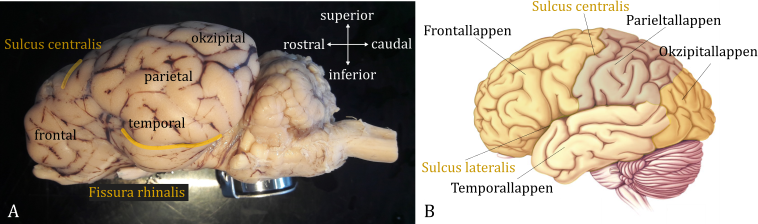
\includegraphics[width=\textwidth]{pictures/Bilder_Jule/Andere/grosshirnrinde.png}
	\caption[Lappen und Sulci der Großhirnrinde]{\textbf{Lappen und Sulci der Großhirnrinde.} \textbf{A:} Großhirnrinde des Schafes, \textbf{B:} Großhirnrinde des Menschen \textsuperscript{\cite[7]{neurowissenschaften_baer}}. Die Großhirnrinde (gelb bis bräunlich) kann anhand der Sulci in vier Lappen (\textit{Lobi cerebri}) unterteilt werden: Frontallappen, Parietallappen, Temporallappen und Okzipitallappen.\index{Lobi cerebri}}
	\label{fig:cortex_lappen} 
\end{figure}

\noindent Die besonders großen und bedeutenden Sulci werden auch Fissuren genannt. Die wohl auffallendste unter ihnen ist die \textbf{Fissura longitudinalis cerebri}\index{Fissura longitudinalis cerebri}. Sie befindet sich zwischen den beiden Großhirnhemisphären. Unter ihr liegt der Corpus callosum\index{Corpus callosum}, die einzige Verbindung der beiden Hemisphären. Der \textbf{Sulcus centralis}\index{Sulcus centralis} erstreckt sich in superior-inferiorer Richtung und trennt den Frontallappen vom Parietallappen. Der \textbf{Sulcus lateralis}\index{Sulcus lateralis} oder auch \textit{Fissura sylvii} erstreckt sich entlang der caudal-rostralen Achse und trennt den Temporallappen vom Frontal- und Parietallappen (Abb.~\ref{fig:cortex_lappen}~B) \textsuperscript{\cite[7]{neurowissenschaften_baer}}. Ein weiterer, bedeutender Sulcus ist die \textbf{Fissura rhinalis}\index{Fissura rhinalis} (Abb.~\ref{fig:cortex_lappen}~A), die den Neocortex räumlich vom Archicortex trennt. 

\subsubsection*{Lappen der Großhirnrinde}
%%%%%%%%%%%%%%%%%%%%%%%%%%%%%%%%%%%%%%%%%%%%%%%%%%%%%%%%%%%

Aufgrund der Gyri und Sulci lässt sich die Großhirnrinde in vier verschiedene Lappen, die \textit{Lobi cerebri}\index{Lobi cerebri}, einteilen (Abb.~\ref{fig:cortex_lappen}). Jedem Lobus können dabei verschiedene Funktionen zugeordnet werden. Der rostral gelegene \textbf{Frontallappen} ist am Kurzzeitgedächtnis, der Planung zukünftiger Handlungen, sowie an der Steuerung der Motorik beteiligt. Der laterale \textbf{Temporallappen} kann mit dem Hören assoziiert werden. Zudem ist er durch die tiefer gelegenen Strukturen des Hippocampus und der Amygdala an Lernvorgängen, Gedächtnisbildung und der Entstehung von Emotionen beteiligt. Der \textbf{Parietallappen} ist caudal hinter dem Frontallappen und superior des Temporallappens lokalisiert. In ihm wird die somatosensorische Wahrnehmung prozessiert. Dabei entsteht ein Eindruck des eigenen Körpers relativ zur räumlichen Umgebung. Der vierte Lobus ist der \textbf{Okzipitallappen}, der sich am caudalen Ende der Großhirnrinde befindet. Er enthält die primären und auch höheren visuellen Areale \textsuperscript{\cite[1]{kandel2013principles}}.

\subsubsection*{Sensorische und Motorische Felder}
\label{subsubsec:Sens_Mot_Felder}
%%%%%%%%%%%%%%%%%%%%%%%%%%%%%%%%%%%%%%%%%%%%%%%%%%%%%%%%%%%

\index{Sensorik !allgemein} In der Großhirnrinde findet die Informationsverarbeitung in verschiedenen Arealen statt. Sie lässt sich funktionell in \textbf{primär motorische}\index{Motorik !allgemein} und \textbf{primär sensorische Felder} unterteilen. Der primäre Motorcortex (M1) enthält Neurone, die an den $\alpha$-Motorneuronen im Ventralhorn des Rückenmarks enden. Er ist rostral des \textit{Sulcus centralis}, auf dem \textit{Gyrus praecentralis}, lokalisiert. Zu den primären sensorischen Feldern gehören der primäre visuelle Cortex (V1) am caudalen Ende des Okzipitallappens, der primäre auditorische Cortex (A1) im Temporallappen, sowie der primäre somatosensorische Cortex (S1) caudal des \textit{Sulcus centralis} auf dem \textit{Gyrus postcentralis}. Alle drei primären sensorischen Felder erhalten hauptsächlich unimodale Information aus den zugehörigen thalamischen Kernen. Dabei ist jedes Sinnesorgan, also Augen, Ohren und die Haut, mehrfach im zugehörigen sensorischen Feld repräsentiert. Diese Repräsentation zeigt dabei eine retinotope, tonotope, bzw. somatotope Organisation. Die \textbf{Topologie}, also die Lagebeziehung, der abgebildeten Information bleibt dabei bestehen. Das Größenverhältnis einzelner Teilgebiete wird dabei nicht zwingend beibehalten \textsuperscript{\cite[14]{penzlin2005tierphys}}. Oft findet eine \textbf{Überrepräsentation} verhaltensrelevanter Bereiche in den primären sensorischen oder motorischen Cortices statt. Beispielsweise werden bei Säugern der retinale Bereich der Fovea im V1 \textsuperscript{\cite{overrepresentation_fovea}}, sowie einige Bereiche der Körperoberfläche in S1 und M1 \textsuperscript{\cite[14]{penzlin2005tierphys}}, überrepräsentiert. Bei einigen Tierarten, wie Fledermäusen, findet zudem eine Überrepräsentation bestimmter auditorischer Frequenzen in A1 statt (\textcolor{red}{Quelle}). Die \textbf{sekundären}, \textbf{tertiären}, usw. \textbf{Repräsentationsfelder} sind den primären untergeordnet. Die sekundären Felder erhalten spezifische thalamische Projektionen.\\

\begin{figure}[H]
    \centering
    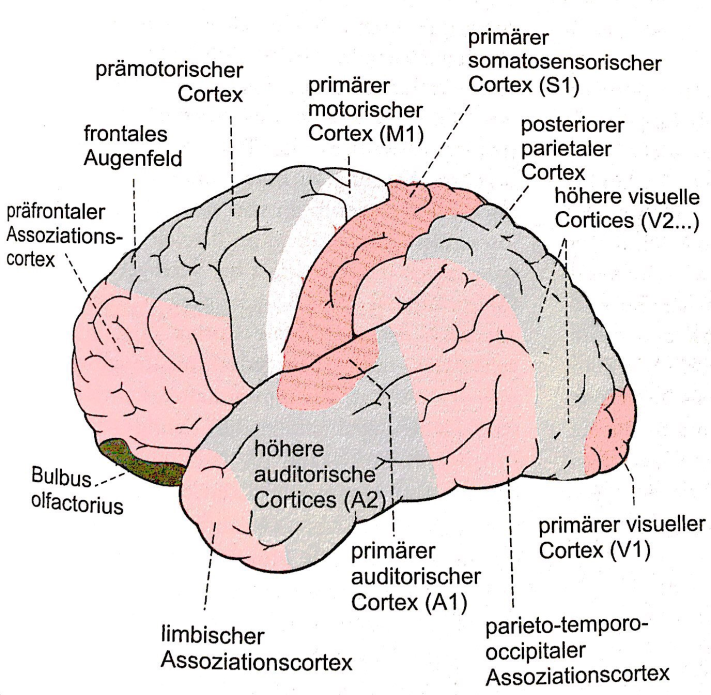
\includegraphics[width=0.7\textwidth]{pictures/Bilder_Jule/Andere/Grosshirnrinde_sensorik_motorik.png}
    \caption[Sensorische, motorische und assoziative Areale der Großhirnrinde]{\textbf{Sensorische, motorische und assoziative Areale der Großhirnrinde.} \textsuperscript{\cite[14]{penzlin2005tierphys}}}
    \label{fig:grosshirnrinde_sensorik_motorik}
\end{figure}

\noindent Jene Felder, die weder den sensorischen noch den motorischen Feldern zugeordnet werden können, werden als sogenannter unspezifischer oder \textbf{assoziativer Cortex} bezeichnet. In diesen Arealen findet eine Verknüpfung oder Integration von motorischer und multisensorischer Information statt \textsuperscript{\cite[14]{penzlin2005tierphys}}. 

\noindent Die Ausdehnung der Projektionsfelder, sowie das Verhältnis zwischen den motorischen und sensorischen Feldern und den Assoziationsfeldern variiert zwischen der verschiedenen Tierklassen: Zum Einen nimmt der Anteil der assoziativen, unspezifischen Felder mit der Höherentwicklung zu \textsuperscript{\cite[14]{penzlin2005tierphys}}. Zum Anderen sind Felder, die für die Lebensweise einer Tierart besonders relevant sind, wie zum Beispiel das olfaktorische Feld bei Ratten, vergrößert (Abb.~\ref{fig:grosshinrinde_vgl}).

\begin{figure}[H]
    \centering
    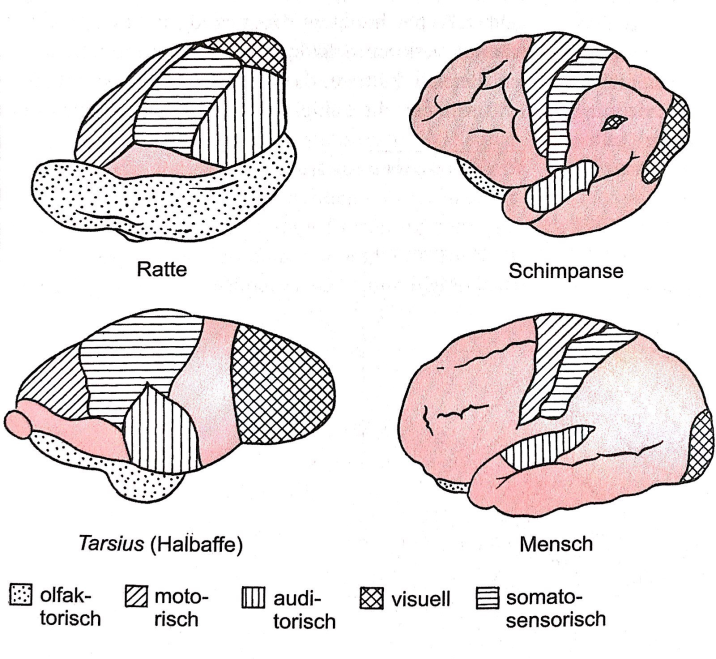
\includegraphics[width=0.7\textwidth]{pictures/Bilder_Jule/Andere/grosshirnrinde_vgl.png}
    \caption[Verhältnis sensorischer, motorischer und assoziativer Areale der Großhirnrinde.]{\textbf{Verhältnis sensorischer, motorischer und assoziativer Areale der Großhirnrinde.} Dargestellt ist die Ausdehnung der sensorischen und motorischen Projektionsfelder (schwarz-weiß) und der assoziativen Felder (rot) verschiedener Säugetiere. \textsuperscript{\cite[14]{penzlin2005tierphys}}}
    \label{fig:grosshinrinde_vgl}
\end{figure}{}


\subsubsection*{Der Neocortex} \index {Neocortex}
%%%%%%%%%%%%%%%%%%%%%%%%%%%%%%%%%%%%%%%%%%%%%%%%%%%%%%%%%%%

Obwohl sich die verschiedenen Areale der Großhirnrinde funktionell unterscheiden und beispielsweise Informationen unterschiedlicher sensorischer Systeme verarbeiten, variiert die Zellschichtung dieser Areale kaum. In evolutionär älteren Arealen des Cortex, wie dem olfaktorischen Cortex, besteht die Großhirnrinde aus nur drei Schichten, während der evolutionär jüngere \textbf{Neocortex}, auch Isocortex, aus sechs Schichten aufgebaut ist. Diese zellulären Schichten bilden die sogenannte \textbf{graue Substanz}\index{graue Substanz} des (Neo-)Cortex, die viele Zellkörper, jedoch wenige Fasern enthält. Diese Schichten werden von Außen nach Innen nummeriert und bestehen aus drei prominenten Zelltypen: exzitatorische Pyramidenzellen, Körnerzellen, zu denen auch die bedornten Sternzellen (\textit{spiny stellate cells}) gehören, und inhibitorische Interneurone. Jede der sechs Zellschichten des Neocortex besitzt charakteristische Zellen und  Verknüpfungen (Abb.~\ref{fig:neoccortex_schichtung}) \textsuperscript{\cite[7]{watson2010thebrain}}. 

\begin{figure}[H]
	\centering
	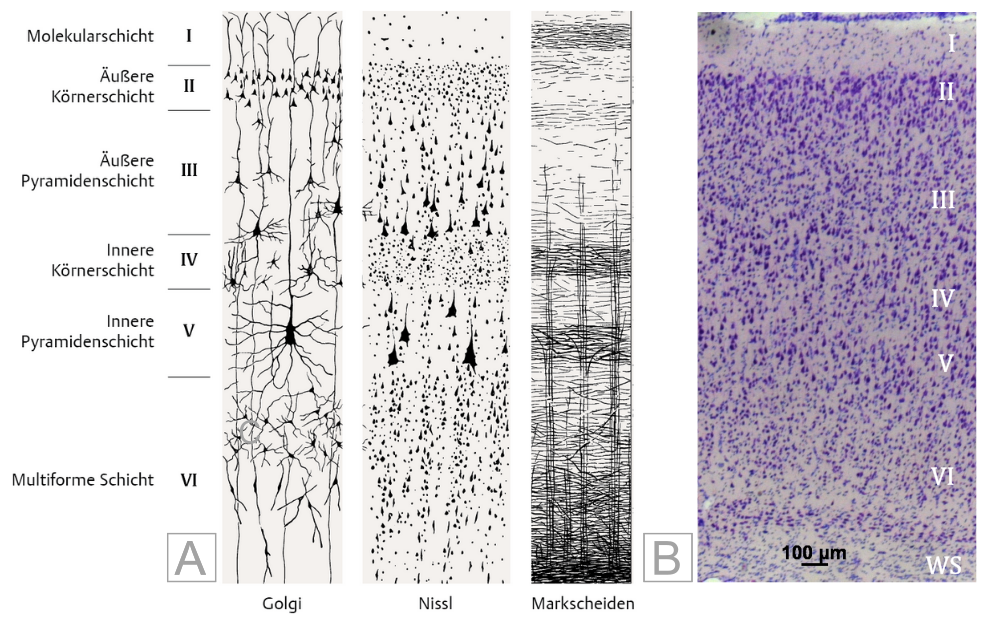
\includegraphics[width=\textwidth]{pictures/Bilder_Jule/Andere/neocortex_schichtung.png}
	\caption[Schichtung des Neocortex]{\textbf{Schichtung des Neocortex.} \textbf{A}:~Schematische Darstellung der Schichten des Neocortex des Menschen unter Verwendung der Golgi-, Nissl- und Markscheidenfärbung \textsuperscript{\cite{taschenbuch_histologie}}. \textbf{B}:~Mikroskopie des Neocortex der Ratte unter Verwendung der Nisslfärbung. WS = weiße Substanz - darüber die sechsschichtige graue Substanz.}
	\label{fig:neoccortex_schichtung}
\end{figure}

\noindent Die \textbf{Molekularschicht} stellt die äußerste Schicht dar. Diese dünne Faserschicht beinhaltet nur wenige Zellkörper, jedoch viele dendritische Fortsätze und stellt somit eine Verarbeitungsstruktur des Cortex dar. Unter ihr liegt die \textbf{äußere Körnerschicht}. Sie besteht aus zahlreichen kleinen Pyramidenzellen sowie kleinen inhibitorischen Zellen. Diese agieren in kleinen neuronalen Schaltkreisen um einkommende Information zu prozessieren. Die dritte Zellschicht, die \textbf{äußere Pyramidenschicht}, zeichnet sich durch eine Vielzahl größerer Pyramidenzellen aus. Diese senden exzitatorische Signale in benachbarte oder auch weit entfernte Areale des Cortex. Korbzellen (\textit{basket cells})  und andere inhibitorische Zellen inhibieren benachbarte Zellen und ermöglichen somit weitere cortikale Informationsverarbeitung. In der vierten Schicht, der \textbf{inneren Körnerschicht}, enden viele thalamische Fasern. Sie besteht aus zahlreichen kleinen Sternzellen. Unter ihr liegt die \textbf{innere Pyramidenschicht}, die aus den größten Pyramidenzellen des Neocortex aufgebaut ist. Ihre Axone, die bis weit außerhalb des Neocortex reichen, terminieren unter anderem im Striatum und Spinalkanal. Die am tiefsten gelegene Schicht ist die sechste, \textbf{multiforme Schicht}. Diese Schicht ist aus vielen kleinen Zellen aufgebaut, unter anderem aus kleinen Pyramidenzellen, die in den Thalamus projizieren. Diese Verbindungen schließen Rückkopplungsschleife zwischen Cortex und Thalamus, der die thalamische Aktivität reguliert \textsuperscript{\cite[7]{watson2010thebrain}}.\\
Die neuronalen Netzwerke, die die corticale Informationsverarbeitung dominieren, zeigen Aktivität, die \textbf{in Säulen organisiert} ist: Die Zellen des Neocortex zeigen die meisten Verbindungen zu Zellen oberhalb und unterhalb der eigenen Position. Dabei weisen einige Zellen inhibitorische Verbindungen zu benachbarten Säulen auf. Diese Verschaltungen scheinen die corticale Aktivität zu fokussieren.\\
\noindent Unterhalb der neocortikalen Schichten liegt die sog. \textbf{weiße Substanz}\index{weiße Substanz} - eine dichte Schicht aus axonalen Fasern, die nur wenige Zellkörper beinhaltet. Diese Fasern ermöglichen die Verbindung und Kommunikation verschiedener Areale des Cortex, sowie die Kommunikation mit dem Rest des Nervensystems \textsuperscript{\cite[7]{watson2010thebrain}}.

\subsubsection*{Der Allocortex} \index{Allocortex}
%%%%%%%%%%%%%%%%%%%%%%%%%%%%%%%%%%%%%%%%%%%%%%%%%%%%%%%%%%%

Der sogenannte Allocortex setzt sich aus dem Archicortex und dem Paleocortex zusammen und ist, genau wie der Neocortex, teil der Großhirnrinde. Der mediale \textbf{Archicortex}\index{Archicortex} der Säugetiere ist aus drei Zellschichten aufgebaut und wird auch Hippocampusregion genannt. Die \textbf{Fissura rhinalis} trennt den evolutionär älteren Archicortex vom jüngeren, sechsschichtigen Neocortex (Abb.~\ref{fig:allocortex_ratte}) \textsuperscript{\cite[6]{storch2012lehrbuchzoo}}. Neben dem Hippocampus ist auch der cinguläre Cortex\index{cingulärer Cortex} (Kap.~\ref{subsubsec:Grosshirnrinde}) ein Teilgebiet des Archicortex. Der lateral gelegene \textbf{Paleocortex}\index{Paleocortex} ist das älteste Teilgebiet der Großhirnrinde. Genau wie der Archicortex besteht er aus drei Zellschichten \textsuperscript{\cite[6]{storch2012lehrbuchzoo}}. Er bildet bei Säugern das Riechhirn und beinhaltet den primären olfaktorischen Cortex, den Bulbus olfactorius\index{Bulbus olfactorius}, sowie die cortikalen Bereiche der Amygdala\index{Amygdala} \textsuperscript{\cite[9]{trepel2011neuroanatomie}}.

\begin{figure}[H]
    \centering
    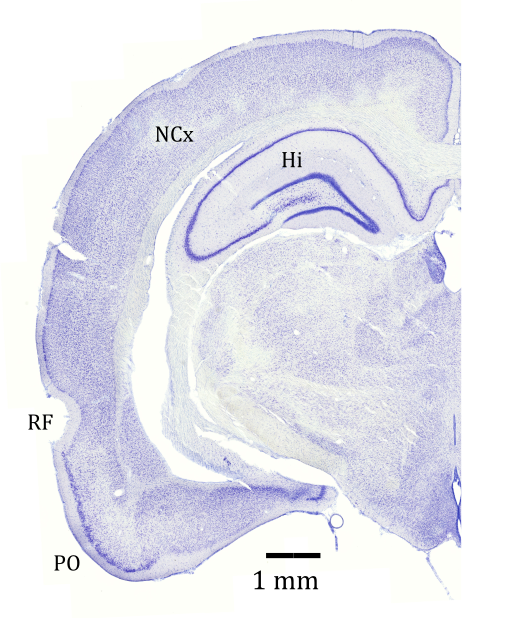
\includegraphics[width=0.4\textwidth]{pictures/Bilder_Jule/Ratte/RF.png}
    \caption[Großhirnrinde Ratte]{\textbf{Großhirnrinde Ratte.} Coronaler Querschnitt durch eine Hemisphäre des Rattengehirns (Nisslfärbung, \textcolor{red}{21-3}). Die superiore Seite ist nach oben, die inferiore nach unten, die laterale nach links und die mediale nach rechts orientiert. Der dreischichtige Hippocampus (\textbf{Hi}) ist Teil des Archicortex, der dreischichtige primäre olfaktorische Cortex (\textbf{CO}) gehört zum Paleocortex. Die Fissura rhinalis (\textbf{RF}) Trennt den sechsschichtigen Neocortex (\textbf{NCx}) vom Paleocortex.}
    \label{fig:allocortex_ratte}
\end{figure}{}

\subsubsection*{Hippocampus}
\label{subsubsec:Hippocampus} \index{Hippocampus}
%%%%%%%%%%%%%%%%%%%%%%%%%%%%%%%%%%%%%%%%%%%%%%%%%%%%%%%%%%%

Das Wort 'Hippocampus' kommt aus dem Griechischen und bedeutet Seepferdchen. Der Hippocampus ist Teil des Archicortex und folglich aus drei Zellschichten ausgebaut. Sowohl bei Menschen als auch bei der Ratte zeichnet sich der Hippocampus durch eine c-förmige Struktur aus, \textsuperscript{\cite[20]{paxinos2014rat}} die den Thalamus umgibt (Abb.~\ref{fig:hippocampus_schaf}). Er hängt dabei am inneren Rand der Großhirnrinde und liegt zum Großteil an den medialen Wänden der lateralen Ventrikel. Caudal reicht der Hippocampus bis vor die Vierhügelplatte. Superior reicht er bis an den \textit{Corpus callosum}, wo er unterhalb des Balkens in die Faserstruktur des \textbf{Fornix}\index{Fornix} übergeht, der bis in den \textbf{Mammillarkörper} zieht. Die \textbf{Fimbria}\index{Fimbria} enthält afferente und efferente Fasern und geht in den Fornix über \textsuperscript{\cite[9]{trepel2011neuroanatomie}}.\\

\begin{figure}[H]
    \centering
    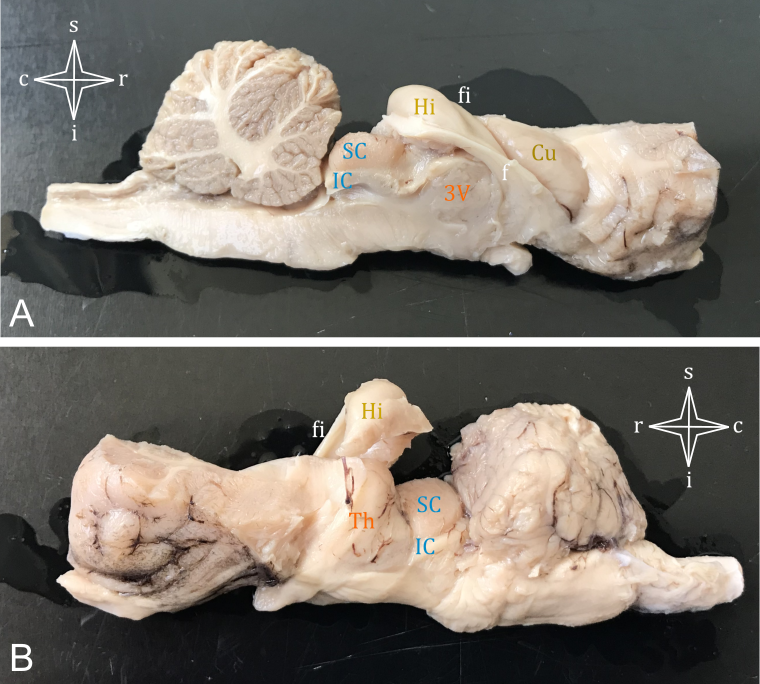
\includegraphics[width=0.6\textwidth]{pictures/Bilder_Jule/Schaf/Ausschnitte/hippocampus_schaf.png}
    \caption[Hippocampus Schaf]{\textbf{Hippocampus Schaf.} Gezeigt ist das Ergebnis einer Hippocampus-Präparation am Schafshirn. Dabei wurden die Bereiche der Großhirnrinde, die den Hippocampus verdecken entfernt. Zu sehen sind der Hippocampus (\textbf{Hi}), der den Thalamus (\textbf{Th}) umschließt. Er liegt caudal des Nucleus caudatus (\textbf{Cu}) und rostral der Vierhügelplatte, die aus dem Colliculus superior (\textbf{SC}) und dem Colliculus inferior (\textbf{IC}) besteht. Ebenfalls gekennzeichnet sind die Fimbria (\textbf{fi}), die in den Fornix (\textbf{f}) übergeht, sowie der dritte Ventrikel (\textbf{3V}), dessen Wände in Teilen vom Thalamus gebildet werden.}
    \label{fig:hippocampus_schaf}
\end{figure}{}

\noindent Die afferenten Fasern, die den Hippocampus erreichen, stammen unter anderem aus dem Neocortex und den olfaktorischen Arealen der Großhirnrinde. Über den Fornix erhält er zusätzlich Informationen aus dem Thalamus, dem cingulären Cortex (\textit{Corpus cinguli}) und der Amygdala. Im Fornix\index{Fornix} verlaufen zudem nahezu alle Efferenzen des Hippocampus. Diese enden unter anderem im Septum, in der Amygdala, sowie im Hypothalamus. Der Großteil der Fasern endet jedoch im Mammillarkörper \textsuperscript{\cite[9]{trepel2011neuroanatomie}}.\\

\noindent Als wichtiger Bestandteil des limbischen Systems (\textcolor{red}{VERWEIS: limb. System}) ist der Hippocampus an emotionalen, endokrinen und vegetativen Vorgängen beteiligt \textsuperscript{\cite[9]{trepel2011neuroanatomie}}. Des Weiteren ist er an der Gedächtnisbildung beteiligt. So ist der Hippocampus beispielsweise für den Transfer von gespeicherter Information vom Kurzzeit- ins Langzeitgedächtnis unabdingbar \textsuperscript{\cite[6]{storch2012lehrbuchzoo}}. Durch synaptische Langzeit-Plastizität wird Information zeitweise im Hippocampus gespeichert. Schließlich werden die Informationen in den Neocortex, den Ort des Langzeitgedächtnisses, transferiert \textsuperscript{\cite[18]{kandel2013principles}}.

\begin{figure}[H]
    \centering
    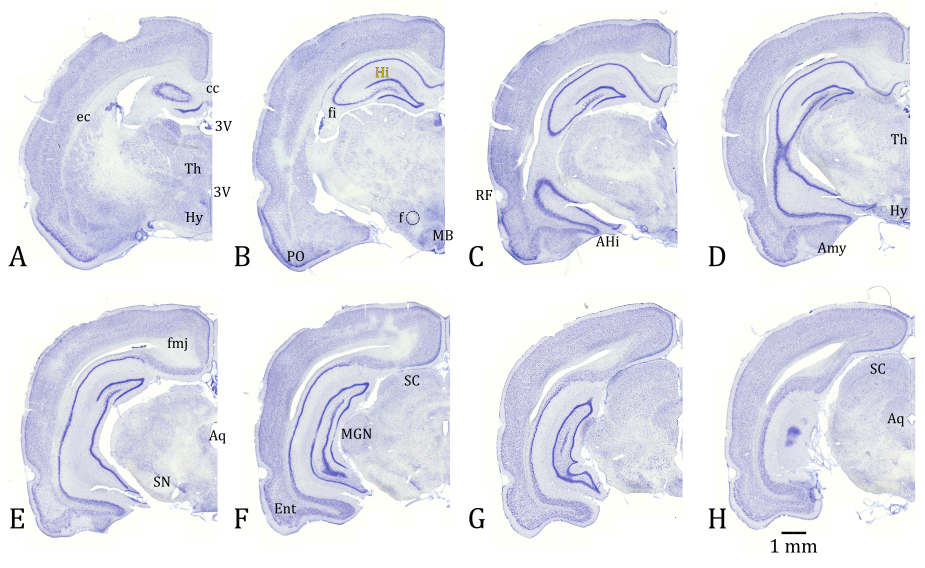
\includegraphics[width=\textwidth]{pictures/Bilder_Jule/Ratte/hippocampus.png}
    \caption[Hippocampus Ratte]{\textbf{Hippocampus Ratte.} Coronalschnitte von rostral nach caudal (Nisslfärbung, \textcolor{red}{A-H: 25-1, 22-2, 20-4, 20-1, 19-1, 18-1, 17-1, 16-1}). Gekennzeichnet sind der Hippocampus (\textbf{Hi}), der den Thalamus (\textbf{Th}) umgibt, sowie die Fimbria (\textbf{fi}) und der Fornix (\textbf{f}). Ebenfalls gekennzeichnete Strukturen des Telencephalons: Capsula externa (\textbf{ec}), Corpus callosum (\textbf{cc}), Forceps minor des cc (\textbf{fmj}), Fissura rhinalis (\textbf{RF}), entorhinaler Cortex  (\textbf{Ent}), primärer olfaktorischer Cortex (\textbf{PO}), amygdalo-hippocampisches Areal (\textbf{AHi}), Amygdala (\textbf{Amy}). Strukturen des Diencephalons: dritter Ventrikel (\textbf{3V}), Hypothalamus (\textbf{Hy}), Mammillarkörper (\textbf{MB}), Corpus geniculatum mediale (\textbf{MGN}). Strukturen des Mesencephalons: Aquädukt (\textbf{Aq}), Colliculus superior (\textbf{SC}), Substantia nigra (\textbf{SN}).}
    \label{fig:hippocampus_ratte}
\end{figure}{}


\subsubsection{Amygdala}
\label{subsubsec:Amygdala} \index{Amygdala}
%%%%%%%%%%%%%%%%%%%%%%%%%%%%%%%%%%%%%%%%%%%%%%%%%%%%%%%%%%%

Die Amygdala (\textit{Corpus amygdaloideum}), auch Mandelkern genannt, liegt unterhalb des olfaktorischen Cortex und rostral des Hippocampus (Abb.~\ref{fig:amygdala_ratte}). Sie ist ein subcortikales Gebiet, das in Teilen dem Paleocortex zuzuordnen ist \textsuperscript{\cite[9]{trepel2011neuroanatomie}}. Die Amygdala ist, wie auch der Hippocampus, wichtiger Teil des limbischen Systems \textsuperscript{\cite[15]{kandel2013principles}} (\textcolor{red}{VERWEIS: limb. System}). 

\begin{figure}[H]
    \centering
    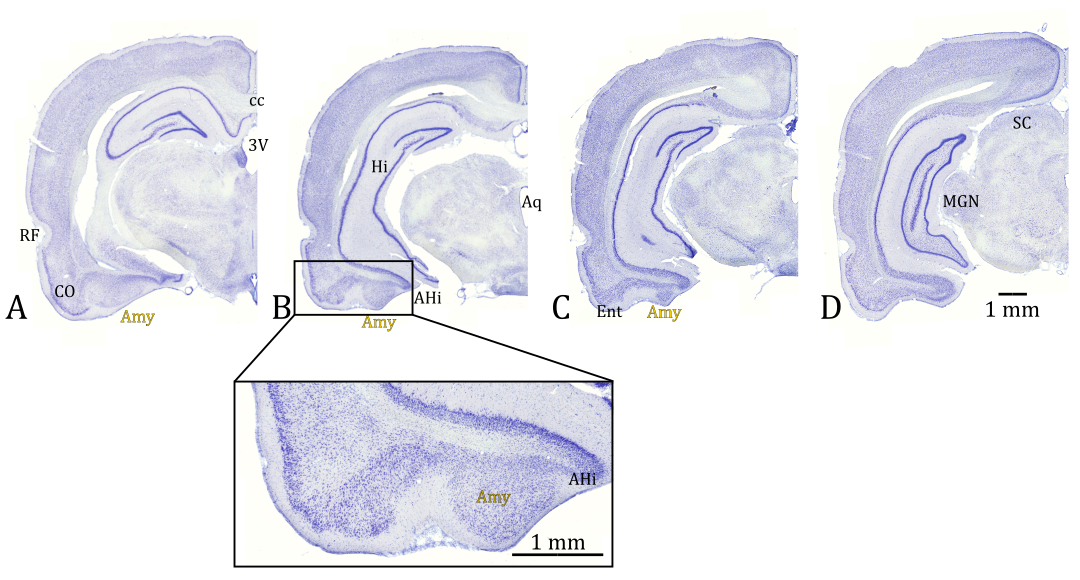
\includegraphics[width=\textwidth]{pictures/Bilder_Jule/Ratte/amygdala.png}
    \caption[Amygdala Ratte]{\textbf{Amygdala Ratte.} Coronalschnitte (Nisslfärbung) von rostral (A) nach caudal (D) \textcolor{red}{(A-D: 20-2, 19-3, 18-4, 17-3)}. Die Amygdala (\textbf{Amy}) liegt unter dem olfaktorischen Cortex (\textbf{CO}). Das amygdalo-hippocampische Areal (\textbf{AHi}) stellt den Übergang zwischen der Amygdala und dem Hippocampus (\textbf{Hi}) dar. Ebenfalls gekennzeichnet sind der Corpus callosum (\textbf{cc}) und die Fissura rhinalis (\textbf{RF}) des Telencephalons, der Corpus geniculatum mediale (\textbf{MGN}) und der dritte Ventrikel (\textbf{3V}) des Diencephalons, sowie das Aquädukt (\textbf{Aq}) und der Colliculus superior (\textbf{SC}) des Mesencephalons.}
    \label{fig:amygdala_ratte}
\end{figure}{}

\noindent Die Amygdala besteht aus mehreren Kernen, die sich in drei Unterbereiche gliedern lassen: Der Zentralbereich steuert vegetative und affektive Grundfunktionen. Der cortikal-mediale Bereich verarbeitet olfaktorische Informationen, wie zum Beispiel soziale Gerüche (Pheromone). Der dritte, basolaterale Teilbereich ist mit Emotionen assoziiert \textsuperscript{\cite[6]{storch2012lehrbuchzoo}}. Im Allgemeinen ist die Amygdala in die Entstehung und Verarbeitung emotionaler Zustände, wie der Angst- und   Vermeidungsreaktion involviert. Sie spielt auch bei positiven Emotionen, besonders wenn das Belohnungssystem involviert ist, eine Rolle \textsuperscript{\cite[48]{kandel2013principles}}.\\

\noindent Die Amygdala erhält direkten und indirekten thalamischen Input. Somit ist sie in der Lage die emotionale Ladung eines Stimulus zu evaluiert. Detektiert sie Gefahr, kann sie, durch ihre starke  Verbindung zu Hypothalamus und Hirnstamm, die Entstehung von physiologischen und endokrinen Antworten und Verhaltensreaktionen dirigieren \textsuperscript{\cite[48]{kandel2013principles}}. Zum Beispiel kann die Amygdala unbewusste Reaktionen auf Angstzustände, wie die Veränderung von Puls, Respirationsrate und Pupillen-Erweiterung,  hervorrufen \textsuperscript{\cite[15]{kandel2013principles}}.
Auch instinktive Prozesse, wie Hunger oder Durst, sowie Prozesse, die Angst-, Aggressions- oder Paarungsverhalten untergeordnet sind, werden von der Amygdala gesteuert \textsuperscript{\cite[18]{kandel2013principles}}.
Die vielseitigen Projektionen, die von der Amygdala ausgehen, erlauben ihr auch andere, kognitive Funktionen zu beeinflussen. Beispielsweise können durch die Amygdala, mittels umfassender Projektionen in cortikale Gebiete, sowohl Aufmerksamkeit, als auch Wahrnehmung, Gedächtnis und Entscheidungsfindung moduliert und somit beeinflusst werden. Durch ihre Verbindung mit den modulatorischen Nuclei, wie Teilen der dopaminergen, noradrenergen und serotonergen Systeme, ist sie zudem in der Lage die kognitive Sachverarbeitung zu beeinflussen \textsuperscript{\cite[48]{kandel2013principles}}.


\subsection{Diencephalon}
\label{subsec:Diencephalon} \index{Diencephalon}
%%%%%%%%%%%%%%%%%%%%%%%%%%%%%%%%%%%%%%%%%%%%%%%%%%%%%%%%%%%
%%%%%%%%%%%%%%%%%%%%%%%%%%%%%%%%%%%%%%%%%%%%%%%%%%%%%%%%%%%

Das Diencephalon oder Zwischenhirn befindet sich caudal, bzw. unterhalb des Telencephalon und umschließt den dritten Ventrikel. Es kann in vier Hauptbereiche gegliedert werden. Von superior nach inferior, bzw. dorsal nach rostral kann zischen \textbf{Epithalamus}, \textbf{Thalamus}, \textbf{Subthalamus}  und \textbf{Hypothalamus} unterschieden werden \textsuperscript{\cite[16]{crossman2014neuroanatomy}}.

\subsubsection{Epithalamus}
\label{subsubsec:Epithalamus} \index{Epithalamus}
%%%%%%%%%%%%%%%%%%%%%%%%%%%%%%%%%%%%%%%%%%%%%%%%%%%%%%%%%%%

Der Epithalamus ist ein kleines Teilgebiet des Diencephalon. Er ist dorsal und caudal gelegen. Bekannte Komponenten des Epithalamus stellen die Epiphyse (Abb.~\ref{fig:schaf_midsagittal}~B,D) und die Nuclei habenulares\index{Nuclei habenulares} (Abb.\ref{fig:Diencephalon_Ratte}~B-D) dar, die mit dem limbischen System in Verbindung stehen \textsuperscript{\cite[12]{crossman2014neuroanatomy}}.\\

\noindent Die \textbf{Epiphyse}\index{Epiphyse} (\textit{Epiphysis cerebri}), auch das \textbf{Pinealorgan} (\textit{Glandula pinealis}) oder die \textbf{Zirbeldrüse}, befindet sich mittig im Diencephalon, direkt rostral des Colliculus superior des Mesencephalon. Bei der Epiphyse handelt es sich um ein unpaares endokrines Organ.
Sie besteht aus Gliazellen und Drüsenzellen, den sogenannten Pinealocyten. Letztere stammen von Photorezeptoren ab und synthetisieren das Hormon Melatonin. Die Epiphyse zeigt, unter anderem  bei bei einigen Fischen, noch netzhautartige Strukturen auf. Bei Säugern ist jedoch keine Photosensibilität mehr vorhanden. Zudem verliert die Epiphyse bei Säugern nach der Geburt ihre neuronale Verbindung zum Gehirn. Durch die Ausschüttung von Melatonin ist sie in die Regulierung des Schlaf-Wach-Rhythmus involviert und somit an der Steuerung des circadianen Rhythmus beteiligt. Auch bei der Regulation des Einsetzens der Pubertät spielt sie eine wichtige Rolle, sowie auch bei der Koordination saisonaler Fortpflanzung \textsuperscript{\cite[13]{penzlin2005tierphys}}.

\subsubsection{Thalamus}
\label{subsubsec:Thalamus} \index{Thalamus}
%%%%%%%%%%%%%%%%%%%%%%%%%%%%%%%%%%%%%%%%%%%%%%%%%%%%%%%%%%%

Der Thalamus stellt die größte Untereinheit des Diencephalon dar. Gemeinsam mit dem Hypothalamus bildet er die laterale Wand des dritten Ventrikels (Abb.~\ref{fig:Diencephalon_Ratte})  \textsuperscript{\cite[12]{crossman2014neuroanatomy}}. \\

\noindent Der Thalamus kann in mehrere kleine Kerngebiete unterteilt werden. Dabei gibt es Nuclei, die sensorische Informationen in die zugehörigen Areale der primären sensorischen Cortices leiten (Abb.~\ref{fig:thalamus_nuclei}) \textsuperscript{\cite[12]{crossman2014neuroanatomy}}. Zu dienen Kerngebieten gehören der \textbf{Corpus geniculatum mediale}\index{Corpus geniculatum mediale, MGN} (MGN) und der \textbf{Corpus geniculatum laterale}\index{Corpus geniculatum laterale, LGN} (LGN). Als Station der Hörbahn leitet der MGN auditorische Information vom Colliculus inferior zur Großhirnrinde weiter. Der LGN stellt eine Station der Sehbahn dar, die zwischen der Retina und dem primären visuellen Cortex liegt \textsuperscript{\cite[14]{penzlin2005tierphys}}. Des Weiteren können Kerngebiete differenziert werden, die Impulse aus Cerebellum und Basalganglia erhalten und an Motorregionen des Frontallappens gekoppelt sind. Zu dem gibt es Nuclei, die Verbindungen zu assoziativen und limbischen Arealen der Großhirnrinde aufzeigen \textsuperscript{\cite[12]{crossman2014neuroanatomy}}.\\

\noindent Im Allgemeinen spielt der Thalamus somit, durch seine reziproken Verbindungen mit dem cerebralen Cortex, eine wichtige Rolle für sensorische, motorische und kognitive Funktionen. Er stellt eine obligatorische Umschalt- und Durchgangszentrale, sowohl motorischer als auch sensorischer Bahnen dar (\textcolor{red}{VERWEIS: Allgemeine sensorische Bahnen}) \textsuperscript{\cite[6]{storch2012lehrbuchzoo}}.

\begin{figure}[H]
    \centering
    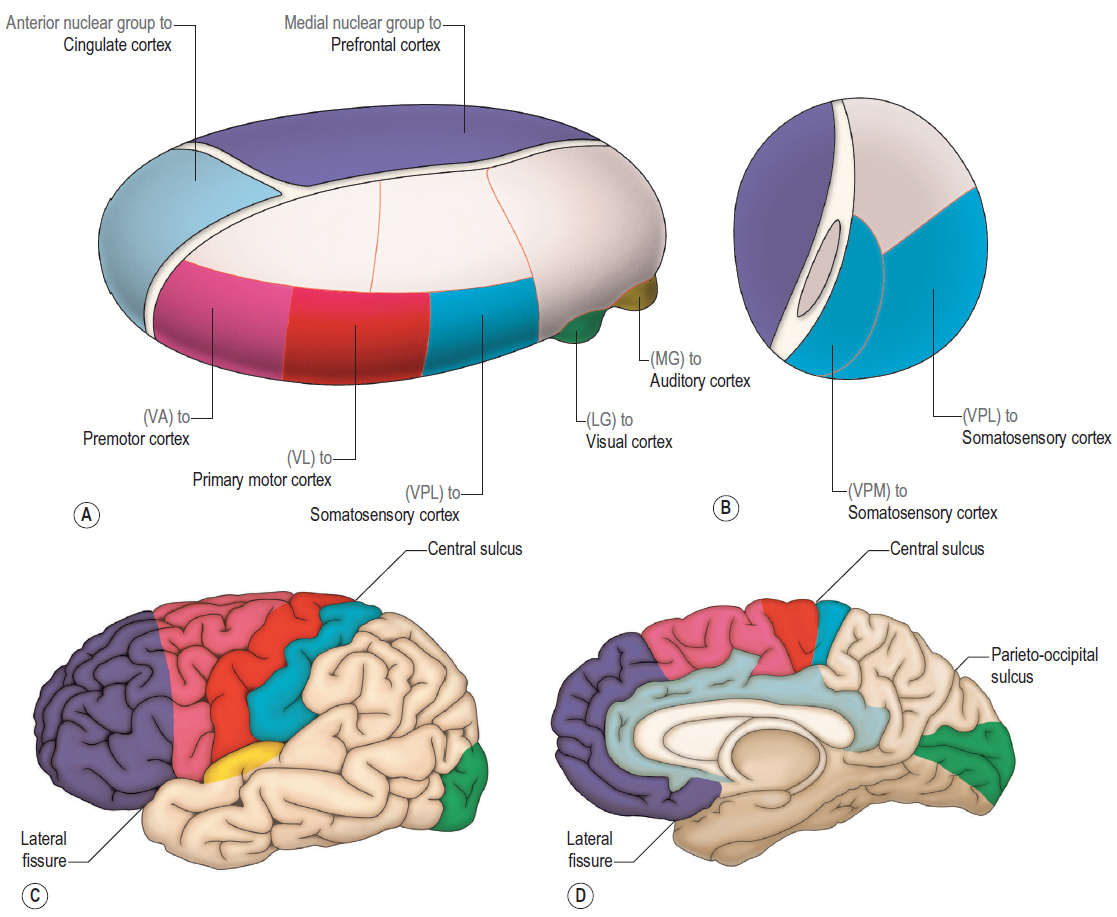
\includegraphics[width=\textwidth]{pictures/Bilder_Jule/Andere/thalamus.png}
    \caption[Projektionen thalamischer Nuclei]{\textbf{Projektionen thalamischer Nuclei.} Dargestellt sind die verschiedenen Teilbereiche des Thalamus, sowie die zugehörigen Areale der Großhirnrinde, mit denen sie in Verbindung stehen. Zum Thalamus gehören unter Anderem der Corpus geniculatum mediale (MGN~- hier MG) und der Corpus geniculatum laterale (LGN~- hier LG). \textbf{A:} anterior-laterale Ansicht, \textbf{B:} Coronalschnitt, \textbf{C:} laterale Ansicht des cerebralen Cortex, \textbf{D:} mediale Aspekte des cerebralen Cortex. Die Farbgebung indiziert die Beziehungen, bzw. Projektionen zwischen den thalamischen Nuclei und den zugehörigen Arealen der Großhirnrinde.\index{Thalamus} \textsuperscript{\cite[12]{crossman2014neuroanatomy}}}
    \label{fig:thalamus_nuclei}
\end{figure}

\subsubsection{Subthalamus} \index{Subthalamus}
%%%%%%%%%%%%%%%%%%%%%%%%%%%%%%%%%%%%%%%%%%%%%%%%%%%%%%%%%%%

Der Subthalamus ist eine kleine Region des Diencephalon. In ihm liegt ventro-lateral der subthalamische Nucleus, der direkt medial der \textit{Capsula interna} liegt. Er zeichnet sich durch neuronale Verbindungen hin zum \textit{Globus pallidus} und der \textit{Substantia nigra} aus. Der subthalamische Nucleus ist an der Kontrolle von Bewegungen beteiligt \textsuperscript{\cite[12]{crossman2014neuroanatomy}} und ähnelt somit funktionell den Basalganglia \textsuperscript{\cite[16]{crossman2014neuroanatomy}}.

\subsubsection{Hypothalamus}
\label{subsubsec:Hypothalamus} \index{Hypothalamus}
%%%%%%%%%%%%%%%%%%%%%%%%%%%%%%%%%%%%%%%%%%%%%%%%%%%%%%%%%%%

Der Hypothalamus bildet die inferiore, bzw. ventrale Wand des dritten Ventrikels, der vom Diencephalon umgeben wird (Abb.~\ref{fig:Diencephalon_Ratte}). Mittig des Hypothalamus geht das \textit{Infundibulum} hervor, das Hypothalamus und Hypophyse miteinander verbindet. Wie auch der Thalamus besteht der Hypothalamus aus mehreren kleineren Kerngebieten. Dazu gehört der \textbf{Mammillarkörper}\index{Mammillarkörper}, auch \textit{Corpus mamillare} (Abb.~\ref{fig:Diencephalon_Ratte}~A, Abb.~\ref{fig:schaf_MB}), der caudal im Hypothalamus gelegen ist und zum limbischen System gehört \textsuperscript{\cite[16]{crossman2014neuroanatomy}}. Beim Menschen, sowie bei Primaten, handelt es sich dabei um eine paarige \textsuperscript{\cite[7]{crossman2014neuroanatomy}}, bei anderen Säugetieren, wie der Ratte, um eine unpaare Struktur \textsuperscript{\cite[13]{paxinos2014rat}}. Der Mammillarkörper erhält Input aus dem Hippocampus über den Fornix (Abb.~\ref{fig:schaf_midsagittal}~B) und ist an der Regulierung des Gedächtnisses beteiligt \textsuperscript{\cite[7]{neurowissenschaften_baer}}. Des Weiteren liegen innerhalb des Hypothalamus neurosekretorische Kerngebiete und die \textbf{Neurohypophyse}\index{Hypophyse !Neurohypophyse}, sowie höhere Koordinationszentren des autonomen Systems \textsuperscript{\cite[6]{storch2012lehrbuchzoo}}.

\begin{figure}[H]
    \centering
    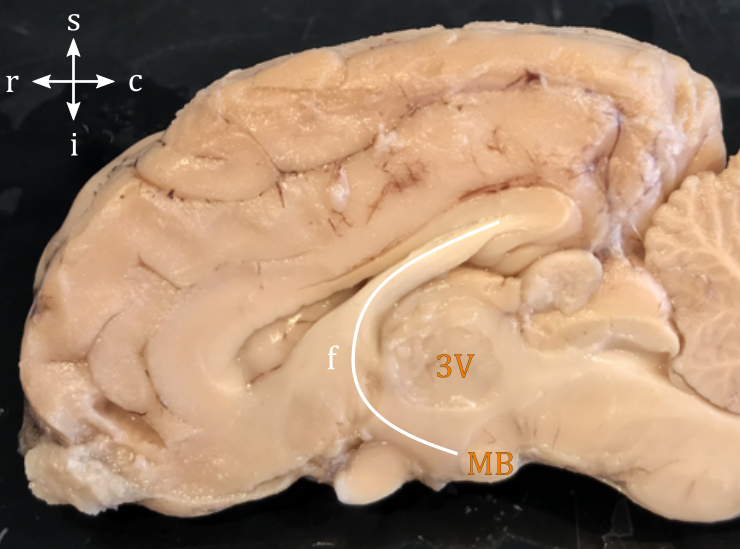
\includegraphics[width=0.5\textwidth]{pictures/Bilder_Jule/Schaf/Ausschnitte/MB.png}
    \caption[Lage der Mammillarkörper]{\textbf{Lage der Mammillarkörper.} Gezeigt ist die Lage des Mammillarkörpers beim Schaf. Die superiore Seite des Gehirns befindet sich dabei oben, die inferiore unten, die rostrale Seite ist nach links, die caudale nach rechts orientiert. Der Mammillarkörper (\textbf{MB}) befindet sich unterhalb des dritten Ventrikels (\textbf{3V}) und steht über den Fornix (\textbf{f}) mit dem Hippocampus in Kontakt.}
    \label{fig:schaf_MB}
\end{figure}{}

\noindent Im Hypothalamus gibt es Thermorezeptoren, die die lokale Temperatur im Hypothalamus wahrnehmen und bei Erwärmung Schwitzen und bei Tieren zudem Hecheln auslösen. Bei Unterkühlung wird Zittern ausgelöst. Osmorezeptoren überwachen die Osmolarität des Blutes, Hormon-Rezeptoren können die Konzentration verschiedener Hormone messen. Dadurch können physiologische Ungleichgewichte erkannt werden, die zu somatosensorischen, vegetativen und endokrinen Reaktionen führen \textsuperscript{\cite[14]{penzlin2005tierphys}}. Beispielsweise wirkt sich die Registrierung von Hunger und Durst auf Appetit und Nahrungsaufnahme aus \textsuperscript{\cite[6]{storch2012lehrbuchzoo}}. Die vielseitigen Reaktionen, die durch den Hypothalamus gesteuert werden, sind durch seine vielseitigen Projektionen möglich. Sie enden unter Anderem im Thalamus, limbischen System, der Hypophyse und dem vegetativen Nervensystem \textsuperscript{\cite[16]{crossman2014neuroanatomy}}. \\

\noindent Diese Vielseitigkeit spiegelt sich auch in den Funktionen des Hypothalamus wieder. Zum einen ist er zusammen mit der Hypophyse\index{Hypophyse} (Hypothalamus-Hypophysen-System), für wichtige, homöostatische Funktionen des Organismus zuständig. Dazu gehört sowohl die Regulation der Körpertemperatur, als auch die des Wasser- und Ionenhaushaltes. Auch ist der Hypothalamus als höchstes Zentrum des vegetativen Nervensystems ein wichtiges Kontrollzentrum für viele Vitalfunktionen \textsuperscript{\cite[14]{penzlin2005tierphys}}. Im Allgemeinen ist er sowohl in Funktionen des autonomen Nervensystems, des limbischen Systems und des neuroendokrinen Systems involviert \textsuperscript{\cite[16]{crossman2014neuroanatomy}}.
 
\begin{figure}[H]
	    \centering
	    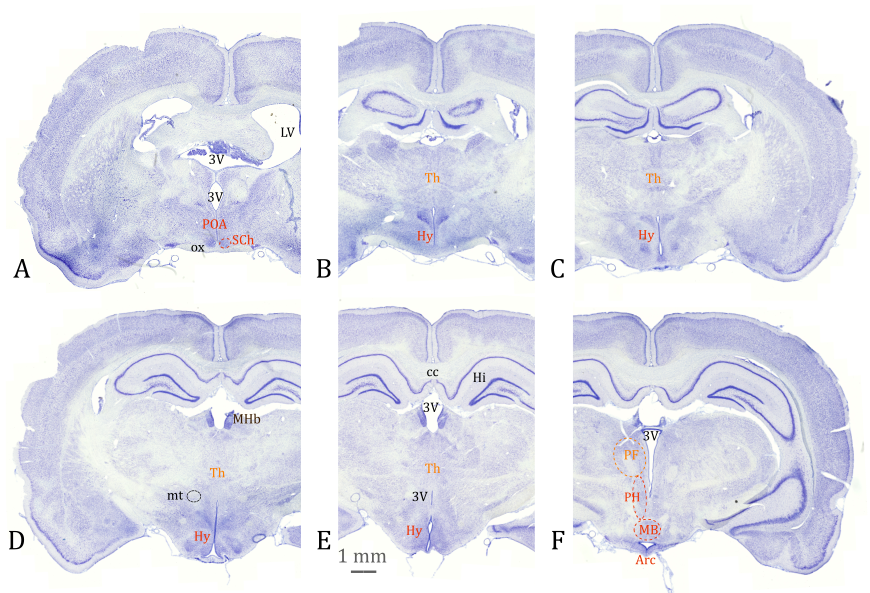
\includegraphics[width=\textwidth]{pictures/Bilder_Jule/Ratte/hypothalamus.png}
	    \caption[Diencephalon Ratte]{\textbf{Diencephalon Ratte.} Gezeigt sind Coronalschnitte (Nisslfärbung) des Rattengehirns von rostral nach caudal \textcolor{red}{(A-F: 16-1, 24-4, 24-1, 22-1, 22-1, 20-3)}. Bereiche des Thalamus (\textbf{Th}) sind in orange gekennzeichnet. Dazu gehören unter Anderem der parafascikuläre thalamische Nucleus (\textbf{PF}). Bereiche des Hypothalamus (\textbf{Hy}) sind rot gekennzeichnet. Dem Hypothalamus sind der Mammillarkörper (\textbf{MB}), der Nucleus arcuatus (\textbf{Arc}), sowie der Nucleus suprachiasmaticus (\textbf{SCh}) und das präoptische Areal\index{präoptisches Areal} (\textbf{POA}) untergeordnet. Ebenfalls Teil des Diencephalon sind das optische Chiasma (\textbf{ox}), der dritte Ventrikel (\textbf{3V}), der mammillo-thalamische Trakt (\textbf{mt}), sowie der (mediale) Nucleus habenulares (\textbf{MHb}), der zum Epithalamus gehört. Ebenfalls gekennzeichnet sind Teile des Telencephalons, wie die lateralen Ventrikel (\textbf{LV}), der Hippocampus (\textbf{Hi}) und der Corpus callosum (\textbf{cc}).\index{Thalamus}\index{Hypothalamus}}
	    \label{fig:Diencephalon_Ratte}
\end{figure}{}



\subsection{Mesencephalon}
\label{subsec:Mesencephalon} \index{Mesencephalon}
%%%%%%%%%%%%%%%%%%%%%%%%%%%%%%%%%%%%%%%%%%%%%%%%%%%%%%%%%%%
%%%%%%%%%%%%%%%%%%%%%%%%%%%%%%%%%%%%%%%%%%%%%%%%%%%%%%%%%%%

Im Mesencephalon ist, ähnlich wie bei der Medulla und dem Rückenmark, eine funktionelle Gliederung in die motorische Grundplatte und die sensorische Flügelplatte erkennbar. Dabei sind die motorischen Kerngebiete ventral, bzw. inferior im Tegmentum gelegen. Die sensorischen Kerngebiete liegen dorsal, bzw. superior im Tectum \textsuperscript{\cite[6]{trepel2011neuroanatomie}}. Das Mesencephalon umgibt das Aquädukt des Ventrikelsystems.

\subsubsection{Tectum: Vierhügelplatte}
\index{Tectum} \index{Vierhügelplatte}
%%%%%%%%%%%%%%%%%%%%%%%%%%%%%%%%%%%%%%%%%%%%%%%%%%%%%%%%%%%

Das Tectum liegt caudal des diencephalen präoptischen Areals und ist dorsal, bzw. superior im Mesencephalon lokalisiert. Es besteht aus der Vierhügelplatte, auch \textit{Lamina tecti} oder \textit{Lamina quadrigemina} genannt. Diese besteht, wie der Name impliziert, aus vier Schwellungen: den paarigen Colliculi superiores und den ebenfalls paarigen Colliculi inferiores \textsuperscript{\cite[6]{trepel2011neuroanatomie}}.

\begin{figure}[H]
    \centering
    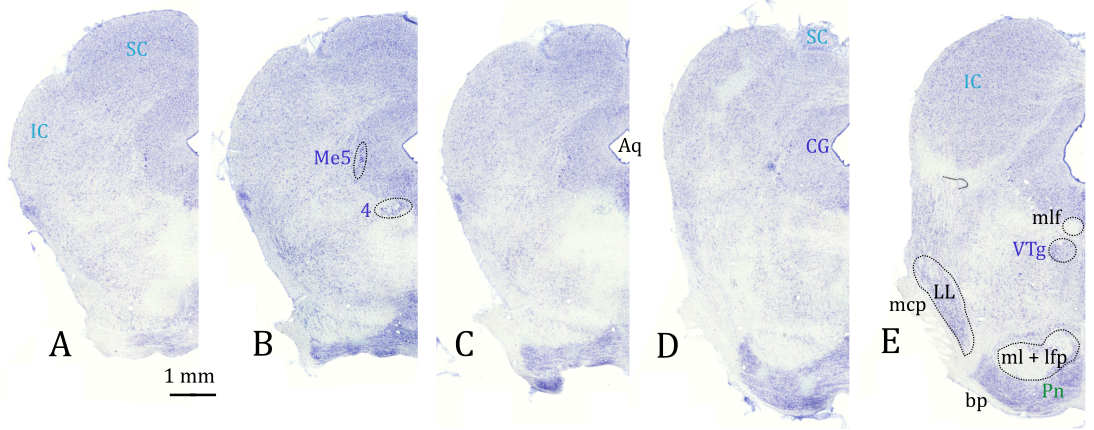
\includegraphics[width=\textwidth]{pictures/Bilder_Jule/Ratte/SC_IC.png}
    \caption[Vierhügelplatte Ratte]{\textbf{Vierhügelplatte Ratte.} Coronalschnitte von caudal nach rostral \textcolor{red}{(Nissl-Färbung: 13-2, 14-1, 14-3, 14-4, 15-1)}. Die superiore Seit zeigt nach oben, die inferiore nach unten. Teile des Cortex, die über dem Mittelhirn liegen, wurden entfernt. Bereiche des Tectum sind hellblau gekennzeichnet. Dazu gehören der Colliculus inferior (\textbf{IC}) und der Colliculus superior (\textbf{SC}). Bereiche des Tegmentums sind dunkelblau markiert. Dazu gehören das Zentraleshöhlengrau (\textbf{Zg}), der Nucleus trochlearis (\textbf{4}), die mesencephalen Nuclei des Nervus trigeminus (\textbf{Me5}), so wie der ventrale Nucleus des Tegmetums (\textbf{VTg}). Ebenfalls zu sehen sind das Aquädukt (\textbf{Aq}) des Mesencephalon und die Nuclei pontis (\textbf{Pn}), die dem Metencephalon zuzuordnen sind. Diese metencephalen Strukturen sind grün gekennzeichnet. Weitere Kennzeichnungen: Nuclei des lateralen Lemniscus (\textbf{LL}), medialer Lemniscus (\textbf{ml}), mediales Kleinhirn-Pedunkel (\textbf{mcp}), medialer longitudinaler Fasciculus (\textbf{mlf}), longitudinaler Fasciculus des Pons (\textbf{lfp}), Brachium pontis (\textbf{bp}). \index{Colliculus superior, SC} \index{Colliculus inferior, IC}}
    \label{fig:vierhuegelplatte_ratte}
\end{figure}{}

\noindent Die geschichteten \textbf{Colliculi superiores}\index{Colliculus superior, SC} enthalten wichtige Kerngebiete, die an der Entstehung und Steuerung der Augenbewegungen beteiligt sind. Über den Nervus opticus, bzw. Tractus opticus erhalten die oberen Colliculi direkte afferente Informationen von der Retina. Weitere Afferenzen kommen über den Tractus corticospinalis aus der Großhirnrinde, über den Tractus spinotectalis aus dem Rückenmark, sowie aus den Colliculi inferiores. Die efferenten Fasern aus den superioren Colliculi ziehen zu den Hirnnervenkernen (Kap.~\ref{subsec:Myelencephalon}), zur Formatio reticularis (Kap.~\ref{subsec:Hirnstamm}) und ins Rückenmark. Funktionell spielen die Colliculi superiores bei der Entstehung visueller Sakkaden, ruckartigen Bewegungen nach Fixationsphasen, eine wichtige Rolle. Auch beim  Akkommodationsreflex, der automatischen Anpassung der Linsenkrümmung um das Abbild der Außenwelt auf der Retina scharf zu stellen, könnten sie beteiligt sein. Zusammengefasst sind die Colliculi superiores in die Entstehung und Steuerung visueller Reflexe und Augenbewegungen involviert \textsuperscript{\cite[6]{trepel2011neuroanatomie}}.\\

\noindent Die \textbf{Colliculi inferiores}\index{Colliculus inferior, IC} liegen direkt inferior der Colliculi superiores. In ihnen werden fast alle Fasern der Hörbahn verschaltet. Somit stellen sie eine wichtige Station der Hörbahn dar (\textcolor{red}{VERWEIS: hörbahn}). Die afferenten Fasern treffen über den lateralen Lemniscus ein. Die efferenten Fasern werden über das Brachium colliculi inferioris zum Corpus geniculatum mediale im Thalamus geleitet \textsuperscript{\cite[6]{trepel2011neuroanatomie}}.


\subsubsection{Tegmentum mesencephali}
\index{Tegmentum !Tegmentum mesencephali}
%%%%%%%%%%%%%%%%%%%%%%%%%%%%%%%%%%%%%%%%%%%%%%%%%%%%%%%%%%%

Der sich im Mesencephalon befindende Teil des Tegmentums befindet sich inferior des Tectums. Es besitzt hauptsächlich motorische Funktionen. So liegen in ihm wichtige Kerngebiete des (extrapyramidalen) motorischen Systems \textsuperscript{\cite[14]{penzlin2005tierphys}}.
Auch die Kerngebiete der Hirnnerven III. (N. oculomotorius) und IV. (N. trochlearis), sowie die motorischen Kerne des Hirnnerven V. (N. trigeminus) sind im mesencephalen Tegmentum lokalisiert \textsuperscript{\cite[6]{trepel2011neuroanatomie}}.\\

\begin{figure}[H]
    \centering
    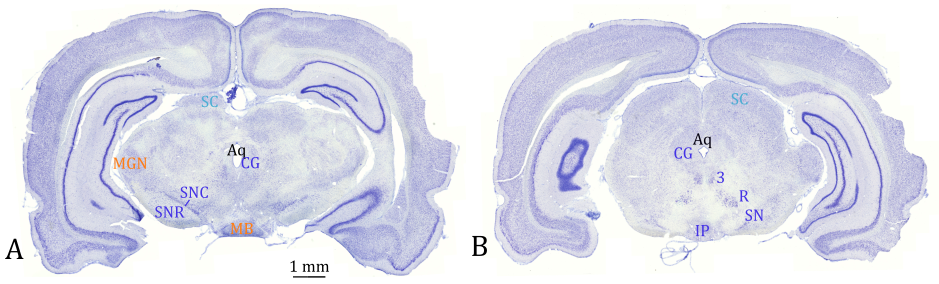
\includegraphics[width=\textwidth]{pictures/Bilder_Jule/Ratte/tegmentum_mesenc.png}
    \caption[Tegmentum Ratte]{\textbf{Tegmentum Ratte.} Coronalschnitte durch das Tegmentum mesencephali. Die Schnitte sind von rostral nach caudal angeordnet (\textcolor{red}{Nissl-Färbung: 18-4, 16-2}). Teilgebiete des Tegmentums sind dunkelblau gekennzeichnet. Dazu gehören das zentrale Höhlengrau (\textbf{CG}), das das Aquädukt (\textbf{Aq}) umgibt, die Substantia nigra (\textbf{SN}), die in die Pars compacta (\textbf{SNP}) und Pars reticulata (\textbf{SNR}) unterteilt ist, sowie der Nucleus ruber (\textbf{R}), die Nuclei des Nervus oculomotorius (\textbf{3}) und der unpaare Nucleus interpeduncularis (\textbf{IP}). Teilgebiete des Tectums, wie die Colliculi superiores (\textbf{SC}) sind hellblau markiert. Rostral sind zudem Teile des Diencephalons (orange), wie der Nucleus geniculatum mediale (\textbf{MGN}) und der Mammillarkörper (\textbf{MB}) zu sehen.}
    \label{fig:tegmentum_mesenc}
\end{figure}{}

\noindent Der \textbf{Nucleus ruber}\index{Nucleus ruber}, ein großer, runder Komplex, ist mittig im Tegmentum mesencephali gelegen. Seine rötliche Färbung ist auf einen hohen Eisengehalt zurückzuführen. Afferenzen erhält der Nucleus ruber aus Cortex und Cerebellum. Efferenzen aus dem N. ruber ziehen über den Tractus rubrospinalis zum Rückenmark, über den Tractus rubroreticularis in die Formatio retucilaris (Kap.~\ref{subsec:Hirnstamm}) und über den Tractus rubroolivaris in die Olive. Funktionell dient der Nucleus ruber als wichtige Schaltstelle des motorischen Systems (\textcolor{red}{VERWEIS: motorik}). Durch seine Projektionen ins Rückenmark ist er Teil des extrapyramidalmotorischen Systems \textsuperscript{\cite[6]{trepel2011neuroanatomie}}.\\

\noindent Auch die \textbf{Substantia nigra}\index{Substantia nigra}, die funktionell den Basalganglia (\textcolor{red}{VERWEIS: Basalganglia}) unterzuordnen ist, ist im Tegmentum lokalisiert. Die dunkle Farbe des Kerngebiets ist durch einen hohen Melanin-Gehalt zu erklären. Generell kann die Substantia nigra in die S.n. \textbf{Pars compacta} und die S.n. \textbf{Pars reticularis} unterteilt werden. Beiden sind unterschiedliche Faserverbindungen und Funktionen zuzuordnen\textsuperscript{\cite[6]{trepel2011neuroanatomie}}. 
Ausgehend von der Substantia nigra pars compacta erstrecken sich Neurone, die Dopamin enthalten, bis hin zu einer Struktur, die \textbf{Area tegmentalis ventralis (VTA)} genannt wird. Die dopaminergen Neurone der VTA sind elementarer Bestandteil des dopaminergen Systems \textcolor{red}{(VERWEIS: dopaminerges System)} \textsuperscript{\cite[9]{crossman2014neuroanatomy}}. Funktionell ist sie in die Kontrolle und Modulation von Bewegungsimpulsen und Bewegungsabläufen involviert. Die Degeneration dopaminerger Neurone der Substantia nigra führt zum Krankheitsbild \textbf{Morbus Parkinson}. Folgen sind Zittern (Tremor) in Ruhephasen, erhöhter Muskeltonus in Verbindung mit steifer Muskulatur (Rigor), sowie Bewegungsarmut (Akinese) \textsuperscript{\cite[6]{trepel2011neuroanatomie}}. \\

\noindent Das \textbf{zentrale Höhlengrau}\index{zentrales Höhlengrau}, auch \textbf{periaquäduktales Grau} oder \textit{Griseum centrale}, ist ein dunkleres, Birnen-förmiges  Kerngebiet, das medial im Mesencephalon liegt. Es umschließt das Aquädukt ähnlich wie die graue Substanz des Rückenmarks den Zentralkanal. Etwa auch gleicher Höhe des superioren und inferioren Colliculus liegen die Nuclei des N. trochlearis und des N. oculomotorius, die äußere Augenmuskulatur innervieren und somit die Augenbewegungen steuern \textsuperscript{\cite[9]{crossman2014neuroanatomy}}. Des Weiteren ist das periaquäduktale Grau Teil des Schmerz-Systems (\textcolor{red}{VERWEIS: pain system?}) \textsuperscript{\cite[25]{paxinos2014rat}}


\subsection{Basalganglia}
\label{subsec:Basalganglia} \index{Basalganglia}
%%%%%%%%%%%%%%%%%%%%%%%%%%%%%%%%%%%%%%%%%%%%%%%%%%%%%%%%%%%
%%%%%%%%%%%%%%%%%%%%%%%%%%%%%%%%%%%%%%%%%%%%%%%%%%%%%%%%%%%

Der Begriff der Basalganglia umschreibt Bestandteile des Tel-, Di- und Mesencephalons.

\begin{wrapfigure}{r}{0.44\textwidth}
    \centering
    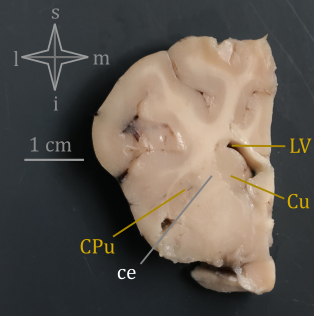
\includegraphics[width=0.42\textwidth]{pictures/Bilder_Jule/Schaf/Ausschnitte/Striatum.png}
    \caption[Striatum Schaf.]{\textbf{Striatum Schaf.} Das Striatum des Schafes besteht aus dem Nucleus caudatus (\textbf{Cu}) und dem Putamen, bzw. Caudoputamen (\textbf{CPu}), die von der Capsula externa (\textbf{ce}), die aus vielen Fasern besteht, voneinander getrennt werden. Der Nucleus caudatus bildet die laterate Seitenwand des dritten Ventrikels (\textbf{3V}).}
    \label{fig:striatum}
\end{wrapfigure}

\noindent Einen Bestandteil der Basalganglia besteht aus dem \textbf{Striatum}, das sich im Telencephalon befindet und bei Säugern in \textbf{Putamen} und \textbf{Nucleus caudatus} unterteilt werden kann. Der Nucleus caudatus legt sich c-förmig um das Putamen, das eine platte Scheibe bildet, und folgt dabei der Oberfläche des lateralen Ventrikels, dessen Seitenwand er bildet. Vor dem Ende des Nucleus caudatus liegt die Amygdala. Auch das \textbf{Pallidum}, auch \textit{Globus pallidus}, das sich im Diencephalon befindet, gehört zu den Basalganglia. Durch die Capsula interna werden Putamen und Pallidum vom Thalamus getrennt (Abb.~\ref{fig:striatum}). Die Capsula interna verläuft auch zwischen dem Putamen und dem Nucleus caudatus. Die einzelnen Bestandteile der Basalganglia erhalten ihre Afferenzen unter anderem aus dem Cortex und den anderen Subbereichen der Basalganglia. Die Efferenzen verlaufen über den Thalamus. Funktionell können den Basalganglia, neben den 'klassischen Bestandteilen', auch der \textbf{Nucleus subthalamus} (Diencephalon) und die \textbf{Substantia nigra} (Mesencephalon) zugeordnet werden.
Im Allgemeinen besteht die Funktion der Basalganglia in der Regulation der Motorik (\textcolor{red}{VERWEIS: Basalganglia}) \textsuperscript{\cite[9]{trepel2011neuroanatomie}}.


\subsection{Rhombencephalon: Metencephalon}
\label{subsec:Metencephalon} \index{Metencephalon}
%%%%%%%%%%%%%%%%%%%%%%%%%%%%%%%%%%%%%%%%%%%%%%%%%%%%%%%%%%%
%%%%%%%%%%%%%%%%%%%%%%%%%%%%%%%%%%%%%%%%%%%%%%%%%%%%%%%%%%%

Das Metencephalon oder auch Hinterhirn ist Teil des Rhombencephalons (Rautenhirn). In seiner Struktur ähnelt es Myelencephalon und Rückenmark. Zwischen Pons und dem Cerebellum, die beide im Metencephalon lokalisiert sind, verläuft der vierte Ventrikel.


\subsubsection{Pons}
\label{subsubsec:Pons} \index{Pons}
%%%%%%%%%%%%%%%%%%%%%%%%%%%%%%%%%%%%%%%%%%%%%%%%%%%%%%%%%%%

Der Pons oder das Brückenhirn beschreibt jenen Teil des Metencephalon, der direkt zwischen Mes- und Myelencephalon und inferior des Cerebellums liegt. Der Pons bildet einen von Außen gut sichtbaren, dicken Wulst, der aus vielen Fasern, aber auch aus grauer Substanz besteht. Im inferioren, bzw. ventralen Bereich, der sogenannten \textbf{Brückenhaube}, liegt das Tegmentum\index{Tegmentum !Tegmentum pontine}, in dem einige Hirnnervenkerne lokalisiert sind. Dazu gehören der Nucleus des N. abducens und des N. facialis. Auch die Nuclei des Trapezkörpers und des medialen Lemniscus sind dort lokalisiert.

\begin{figure}[H]
    \centering
    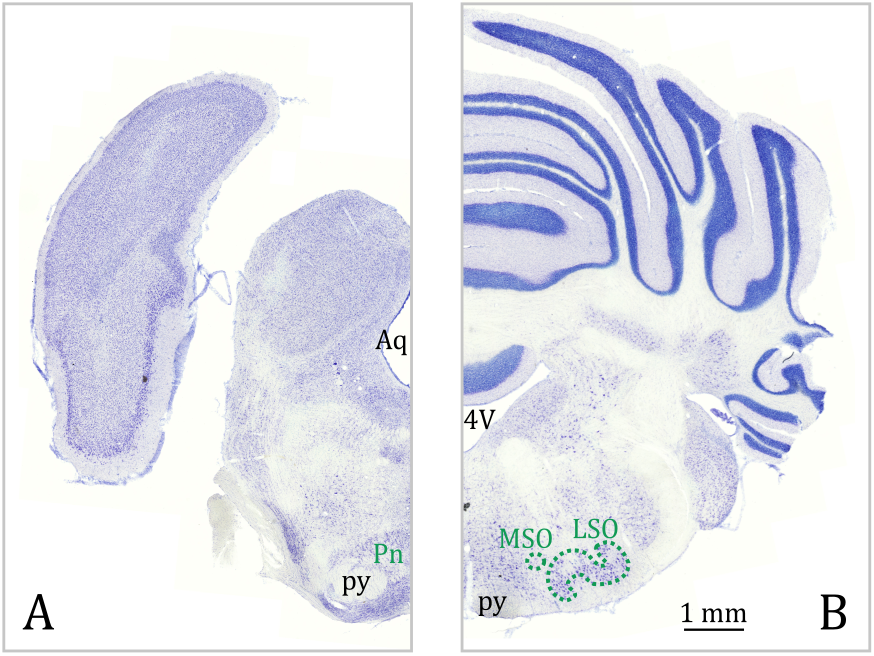
\includegraphics[width=0.7\textwidth]{pictures/Bilder_Jule/Ratte/pons.png}
    \caption[Pons Ratte]{\textbf{Pons Ratte.} Dargestellt sind ein rostraler (A) \textcolor{red}{(Nissl-Färbung: 12-2)} und caudaler (B) \textcolor{red}{(8-2)} Querschnitt durch den Pons. Dabei ist rostral über dem Pons noch das Mesencephalon zu sehen, durch das sich das Aquädukt (\textbf{Aq}) zieht. Über dem Mesencephalon sind Teile des Cortex sichtbar. In diesem Bereich des Pons befinden sich die Nuclei pontis (\textbf{Pn}). Im caudalen Querschnitt ist am oberen Ende das Cerebellum sichtbar. Auch der vierte Ventrikel (\textbf{4V}) ist zu sehen, sowie die mediale (\textbf{MSO}) und laterale obere Olive (\textbf{LSO}). Die Pyramidenbahn (\textbf{py}) liegt im ventralen Teil des Pons und erstreckt sich über dessen gesamte Länge.}
    \label{fig:pons_ratte}
\end{figure}{}

\noindent Der superiore Bereich wird auch \textbf{Brückenbasis} genannt. Sie beinhaltet die \textbf{Pyramidenbahn} und den \textbf{oberen Olivenkomplex}\index{Olive !obere Olive} (\textit{Nucleus olivaris superior}), der eine wichtige Station der Hörbahn darstellt. Ebenfalls im Pons liegen die \textbf{Nuclei pontis}\index{Nuclei pontis}, auch Brückenkerne genannt. Diese Nuclei sind von den Fasermassen, die ihnen entspringen, bzw. zu ihnen führen, umgeben. Die meisten Afferenten erhalten sie über den Tractus corticopontinus. Dieser Trakt führt Fasern aus diversen Großhirnbereichen. Dabei erhalten die Nuclei unter anderem Informationen über Bewegungsentwürfe, die im prämotorischen Cortex ausgearbeitet werden. Nach dem die Fasern innerhalb des Pons auf die kontralaterale Seite kreuzen, enden die Efferenzen in der kontralateralen Kleinhirnhemisphäre. So können die Nuclei pontis die erhaltenen Informationen zur weiteren Feinabstimmung an das Kleinhirn weiterleiten. Die Nuclei pontis spielen somit eine entscheidende Rolle  bei der Verschaltung von Informationen aus dem Großhirn zum Kleinhirn \textsuperscript{\cite[5]{trepel2011neuroanatomie}}.

\subsubsection{Cerebellum}
\label{subsubsec:Cerebellum} \index{Cerebellum !allgemein}
%%%%%%%%%%%%%%%%%%%%%%%%%%%%%%%%%%%%%%%%%%%%%%%%%%%%%%%%%%%

Das Cerebellum oder Kleinhirn ist dorsal oder superior im Metencephalon über dem Hirnstamm gelegen. Somit bedeckt es dorsal den vierten Ventrikel. Es ist durch drei Kleinhirnstiele, die \textit{Pedunculi cerebellaris}\index{Kleinhirnpedunkel}, mit dem Hirnstamm verbunden. Über diese Stiele verlaufen sowohl die Afferenzen als auch die Efferenzen des Cerebellums. Zudem ziehen zwei Kleinhirnsegel (\textit{Velum})\index{Velum} zum Mesencephalon und der Medulla. Diese Veli bestehen aus weißer Substanz und bilden das Dach des vierten Ventrikels. Bei lissencephalen\index{lissencephal} Spezies weist das Cerebellum, ähnlich wie die Großhirnrinde, viele Faltungen auf. Im direkten Vergleich sind die Falten des Cerebellums deutlich kleiner und zahlreicher. Sie verlaufen horizontal und werden auch als Blätter (\textit{Foliae}) bezeichnet \textsuperscript{\cite[7]{trepel2011neuroanatomie}}. Eine weitere Ähnlichkeit zum Cortex besteht in der Schichtung des Cerebellums. Wie Teile der  Großhirnrinde ist auch das Kleinhirn aus drei Zellschichten aufgebaut. Die äußerste Schicht ist die \textbf{Molekularschicht} unter der die \textbf{Purkinje-Zellschicht} liegt. Die innerste Schicht ist die \textbf{Körnerzellschicht} (Abb.~\ref{fig:cerebellum_ratte}) \textsuperscript{\cite[14]{penzlin2005tierphys}}.

\begin{figure}[H]
    \centering
    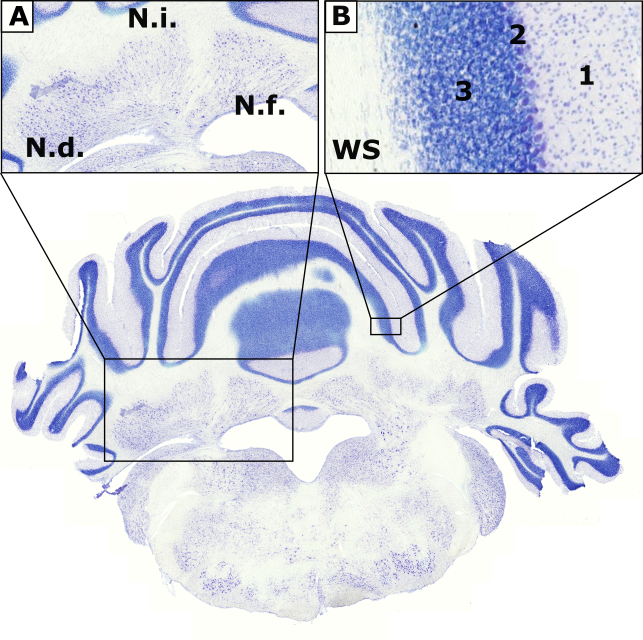
\includegraphics[width=\textwidth]{pictures/Bilder_Jule/Ratte/cerebellum.png}
    \caption[Schichtung Cerebellum]{\textbf{Schichtung Cerebellum.} Ausschnitt des caudalen Cerebellums, unter dem sich die Medulla befindet. Zwischen Medulla und Cerebellum ist der vierte Ventrikel sichtbar. Gekennzeichnet sind die weiße Substanz (\textbf{WS}), sowie die drei Schichten der grauen Substanz. Die äußerste Schicht ist die Molekularschicht (\textbf{1}). Weiter innen liegen die Purkinje-Zellschicht (\textbf{2}) und die Körnerzellschicht (\textbf{3}).}
    \label{fig:cerebellum_ratte}
\end{figure}

\noindent Aufgrund der verschiedenen afferenten Faserverbindungen lässt sich das Cerebellum in drei Gebiete gliedern: Das \textbf{Vestibulocerebellum}\index{Cerebellum !Vestibulocerebellum} erhält Afferenzen aus aus dem Vestibularapparat des Innenohrs, das \textbf{Spinocerebellum}\index{Cerebellum !Spinocerebellum} aus dem Rückenmark und das \textbf{Pontocerebellum}\index{Pontocerebellum} aus den Nuclei pontis \textcolor{red}{(VERWEIS: MOTOR-Cerebellum)}. Des Weiteren liegen im Cerebellum die \textbf{Keinhirnkerne}, zu denen der Nucleus dentatus, der Nucleus emboliformis, sowie der Nucleus globosus und der Nucleus fastigii gehören. Das Cerebellum spielt eine wichtige Rolle für die Koordination von Haltung und Bewegung und gilt generell als motorisches Koordinationszentrum \textsuperscript{\cite[7]{trepel2011neuroanatomie}}.




\subsection{Rhomencephalon: Myelencephalon}
\label{subsec:Myelencephalon} \index{Myelencephalon}
%%%%%%%%%%%%%%%%%%%%%%%%%%%%%%%%%%%%%%%%%%%%%%%%%%%%%%%%%%%
%%%%%%%%%%%%%%%%%%%%%%%%%%%%%%%%%%%%%%%%%%%%%%%%%%%%%%%%%%%

\subsubsection{Medulla} \index{Medulla oblongata}
%%%%%%%%%%%%%%%%%%%%%%%%%%%%%%%%%%%%%%%%%%%%%%%%%%%%%%%%%%%

Das Myelencephalon (Nachhirn) besteht aus der \textbf{Medulla oblongata}, auch verlängertes Rückenmark genannt. Sein 'Dach' ist dünn und weist kleine Falten auf \textsuperscript{\cite[6]{storch2012lehrbuchzoo}}. Die Medulla liegt caudal des Pons und leitet zum Rückenmark über, dem es sowohl in Aufbau als auch Funktion ähnelt (Abb.~\ref{fig:medulla_schema},~\ref{fig:ruckenmark_schema}). Genau wie im Rückenmark sind die sensorischen Regionen dorsal im Hinterhorn (Flügelplatte) und die motorischen Regionen ventral im Vorderhorn (Grundplatte) in der grauen Substanz lokalisiert. Dabei liegen die somatosensorischen Regionen eher lateral, die viscerosensorischen Regionen eher medial. Im Vergleich zum Rückenmark ist der Zentralkanal erweitert und bildet den vierten Ventrikel. Beim Übergang von Rückenmark zur Medulla geht die dorso-ventrale Organisation des Rückenmarks in eine eher medio-laterale  Organisation über \textsuperscript{\cite[14]{penzlin2005tierphys}}.

\begin{figure}[H]
    \centering
    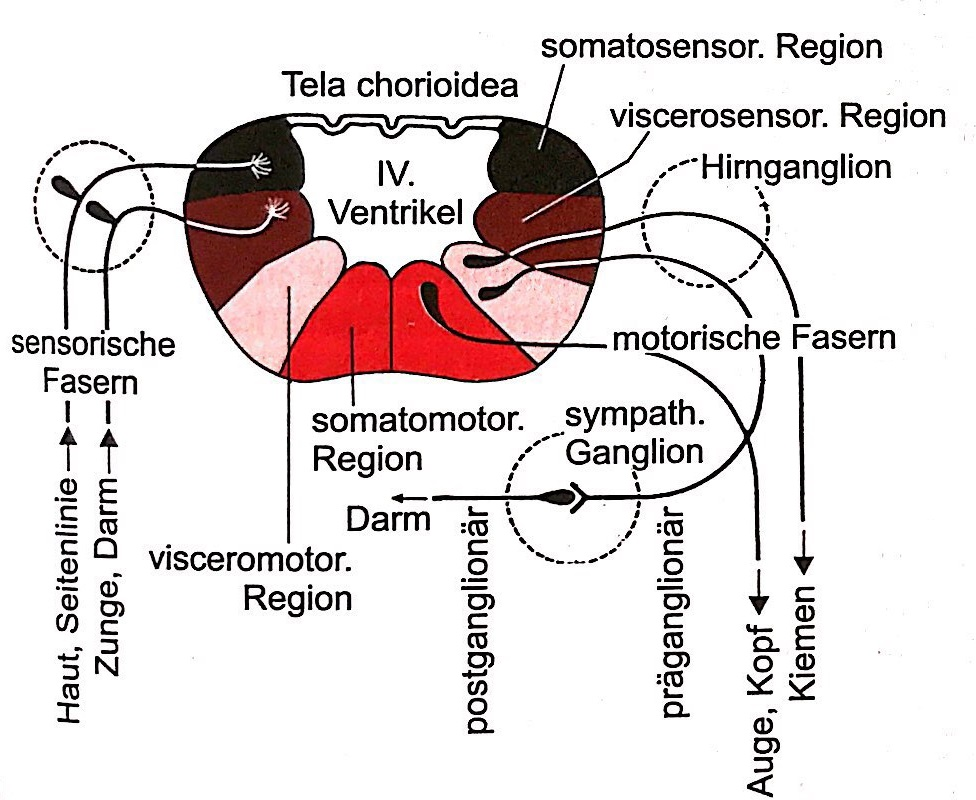
\includegraphics[width=0.6\textwidth]{pictures/Bilder_Jule/Andere/medulla_schema.jpg}
    \caption[Aufbau der Medulla]{\textbf{Aufbau der Medulla.} Gezeigt ist ein schematischer Querschnitt durch die Medulla, bzw. den Hirnstamm. Die superiore, bzw. dorsale, sensorische Seite ist nach oben, die inferiore, bzw. ventrale, motorische Seite nach unten orientiert. {\textsuperscript{\cite[14]{penzlin2005tierphys}}}}
    \label{fig:medulla_schema}
\end{figure}{}

\noindent Im Vergleich zu den anderen Hirnarealen entspringen der Medulla die meisten Hirnnerven (Abb.~\ref{fig:hirnnerven_schaf}). So liegen sowohl die primären sensorischen, als auch die primären motorischen Kerngebiete der Hirnnerven IV bis XII in der Medulla \textsuperscript{\cite[14]{penzlin2005tierphys}}. Neben zahlreichen Hirnnervenkernen ist auch die \textbf{inferiore Olive}\index{Olive !untere Olive}, ein Kerngebiet, das in die Motorkontrolle involviert ist (\textcolor{red}{VERWEIS: Motorsystem?})  \textsuperscript{\cite[9]{crossman2014neuroanatomy}}, in der Medulla lokalisiert. Auch die Hinterstrangkerne, der \textbf{Nucleus cuneatus}\index{Nucleus cuneatus} und der \textbf{Nucleus gracilis}\index{Nucleus gracilis}, die Stationen der somatosensorischen Bahn darstellen (\textcolor{red}{VERWEIS:  Tastsinn}) \textsuperscript{\cite[5]{trepel2011neuroanatomie}} und der Cochleare Nucleus\index{cochlearer Nucleus}, sind in der Medulla lokalisiert (Abb.~\ref{fig:medulla_ratte}). Zusammen mit dem Pons\index{Pons} besteht die Funktion des Myelencephalon unter anderem in der Regulation von Atmung und Kreislauf \textsuperscript{\cite[14]{penzlin2005tierphys}}.

\begin{figure}[H]
    \centering
    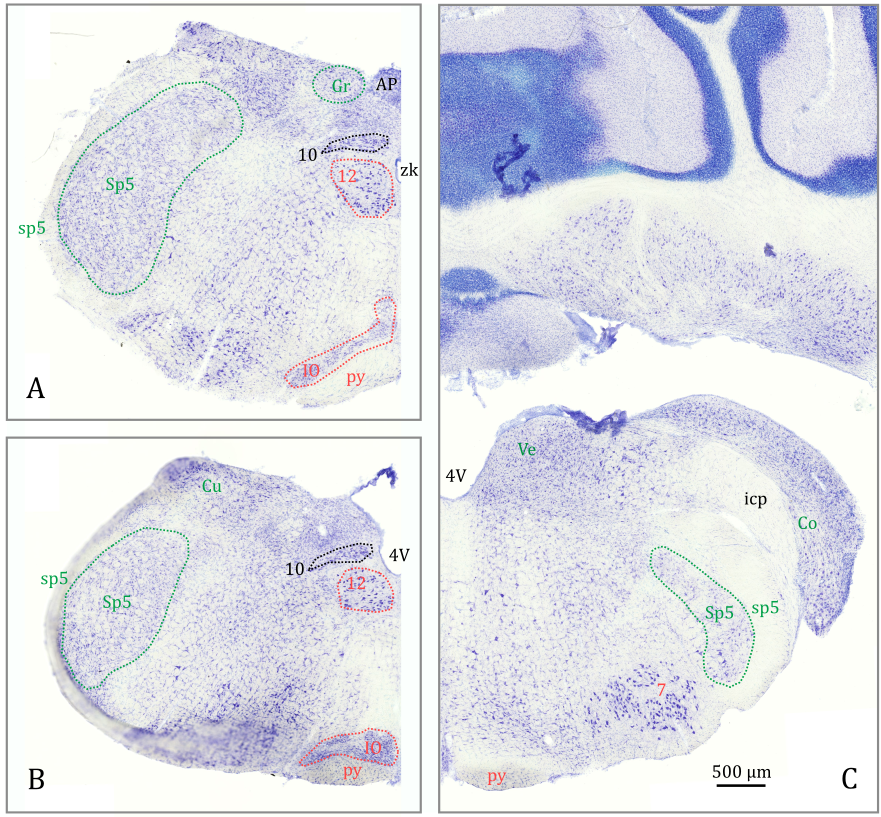
\includegraphics[width=\textwidth]{pictures/Bilder_Jule/Ratte/medulla.png}
    \caption[Medulla Ratte]{\textbf{Medulla Ratte.} Gezeigt sind Querschnitte durch die Medulla (Nissl-Färbung). \textbf{A} ist caudaler (\textcolor{red}{1-4}), \textbf{B} rostraler (\textcolor{red}{2-4}) lokalisiert. Auf \textbf{C}, dass sich weiter rotral befindet (\textcolor{red}{6-1}) ist oben bereits das Cerebellum sichtbar. Sensorische Gebiete sind grün gekennzeichnet. Dazu gehören der Spinalkanal des N. trigeminus (\textbf{sp5}), sowie die zugehörigen Nuclei (\textbf{Sp5}), der Nucleus cochlearis (\textbf{Co}), der Nucleus vestibularis (\textbf{Ve}), sowie die Hinterstrangkerne: der Nucleus cuneatus (\textbf{Cu}) und der Nucleus gracilis (\textbf{Gr}). Motorische Gebiete sind rot markiert. Dazu gehören die Nuclei des N. hypoglossus (\textbf{12}), die Pyramidenbahn (\textbf{py}) und die inferiore Olive (\textbf{IO}). Ebenfalls gekennzeichnet sind die Nuclei des Vagus Nervs (\textbf{10}), der sowohl sensorische als auch motorische Funktionen besitzt, das Pedunculus cerebellaris inferior (\textbf{icp}), der Zentralkanal (\textbf{zk}) und der vierte Ventrikel (\textbf{4V}).} 
    \label{fig:medulla_ratte}
\end{figure}{}


\subsection{Hirnstamm}
\label{subsec:Hirnstamm} \index{Hirnstamm}
%%%%%%%%%%%%%%%%%%%%%%%%%%%%%%%%%%%%%%%%%%%%%%%%%%%%%%%%%%%
%%%%%%%%%%%%%%%%%%%%%%%%%%%%%%%%%%%%%%%%%%%%%%%%%%%%%%%%%%%

Unter dem Begriff Hirnstamm (\textit{Truncus cerebri}) werden die ventralen Bereiche des Mittelhirns (Mesencephalon), des Hinterhirns (Metencephalon) und des Nachhirns (Myelencephalon) zusammengefasst. Es besteht somit aus Teilen des Mittelhirns, sowie aus dem Pons und der Medulla. Rostral, vor dem Hirnstamm, liegt das Zwischenhirn (Diencephalon), caudal, hinter dem Hirnstamm, folgt das Rückenmark. Im Hirnstamm sind motorische Zentren lokalisiert, die für die Kontrolle der Körperhaltung und Bewegung zuständig sind. Diese Bereiche werden im Allgemeinen auch als \textbf{Tegmentum} bezeichnet. Es kann, dem Verlauf des Ventrikelsystems folgend, in drei Unterbereiche gegliedert werden: Das \textit{Tegmentum mesencephali}\index{Tegmentum !Tegmentum mesencephali} befindet sich im ventralen, bzw. inferioren Mittelhirn \textsuperscript{\cite[6]{trepel2011neuroanatomie}}. Das \textit{Tegmentum pontine}\index{Tegmentum mesencephali} ist ebenfalls ventral gelegen und befindet sich im Pons. Der Bereich des Tegmentums, der sich in der Medulla befindet, wird \textit{Tegmentum myelencephali}\index{Tegmentum !Tegmentum myelencephali} genannt. Im Vergleich zum Mes- und Metencephalon ist das Tegmentum im Myelencephalon dorsal, bzw. superior gelegen \textsuperscript{\cite[5]{trepel2011neuroanatomie}}.\\

\noindent Doch der Hirnstamm besitzt neben den motorischen auch andere Funktionen. So liegen in ihm auch relativ autonome, vegetative Zentren, die beispielsweise Atem- und Kreislaufsystem steuern \textsuperscript{\cite[14]{penzlin2005tierphys}}. Eines dieser Zentren ist die \textbf{Formatio reticularis}\index{Formatio reticularis}. Sie erstreckt sich vom Mesencephalon über den Pons und die Medulla bis hinab ins Rückenmark. Durch die Formatio reticularis werden sowohl sympathische als auch parasympathische Zentren gesteuert. Sie selbst wird vom Hypothalamus kontrolliert. Funktionell lässt sich die Formatio reticularis in eine Vielzahl kleinerer Zentren unterteilen. Sowohl motorische Zentren, wie das sogenannte Motorische Zentrum und das Augenbewegungszentrum, als auch Kreislauf- und Atemzentren sind in ihr lokalisiert. Des Weiteren beinhaltet sie das sogenannte Brechzentrum und das Miktionszentrum \textsuperscript{\cite[6]{trepel2011neuroanatomie}}.


\subsection{Rückenmark}
\label{subsec:Rueckenmark} \index{Rückenmark}
%%%%%%%%%%%%%%%%%%%%%%%%%%%%%%%%%%%%%%%%%%%%%%%%%%%%%%%%%%%
%%%%%%%%%%%%%%%%%%%%%%%%%%%%%%%%%%%%%%%%%%%%%%%%%%%%%%%%%%%

Das Rückenmark zeigt eine dorso-ventrale Organisation auf (Abb.~\ref{fig:ruckenmark_schema}). Dabei weist die zentral gelegene \textbf{graue Substanz}\index{graue Substanz}, die den Zentralkanal umgibt und die Somata der vorliegenden Neurone enthält, eine typische Schmetterlingsform auf. Generell kann zwischen dem Vorder- und Hinterhorn des Rückenmarks unterschieden werden. Im ventralen Vorderhorn (Grundplatte) sind die Somata der motorischen Fasern lokalisiert. Dabei sind die somatomotorischen Neurone eher dorsal, die visceromotorischen eher dorso-lateral gelegen. Im dorsalen Hinterhorn (Flügelplatte), in dem die Somata der sensorischen Neurone liegen, sind die somatosensorischen Neurone eher ventral gelegen, die viscerosensorischen eher dorsal.\\

\noindent Die \textbf{weiße Substanz}\index{weiße Substanz} umgibt peripher die graue Substanz. Sie enthält neben Gliazellen und Blutgefäßen ausschließlich markhaltige Fasern. Dabei verlaufen sowohl die aufsteigenden, als auch die absteigenden Bahnen in der weißen Substanz. Des Weiteren treten pro Körpersegment jeweils zwei laterale Nerven aus, die \textbf{dorsale und ventrale Wurzel} genannt werden (Abb.~\ref{fig:ruckenmark_schema}). Diese vereinen sich in kurzem Abstand zum Rückenmark zu \textbf{Spinalnerven}. Kurz vor dieser Vereinigung von dorsaler und ventraler Wurzel ist eine Schwellung erkennbar, das sogenannte \textbf{Spinalganglion}. Dieses dient der metabolischen Versorgung, sowie der Energieversorgung der vorliegenden Neurone. Nach der Vereinigung zum Spinalnerv spaltet sich dieser erneut in drei Äste (Rami) auf (Abb.~\ref{fig:ruckenmark_wirbelsaeule}) \textsuperscript{\cite[14]{penzlin2005tierphys}}.

\begin{figure}[H]
     \centering
     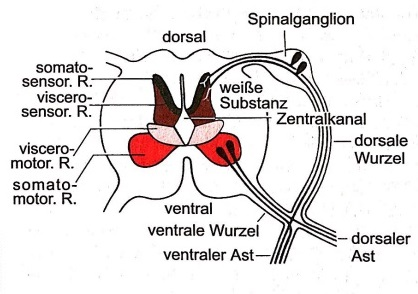
\includegraphics[width=0.6\textwidth]{pictures/Bilder_Jule/Andere/rueckenmark_schema.jpg}
     \caption[Aufbau des Rückenmarks]{\textbf{Aufbau des Rückenmarks.} Gezeigt ist ein schematischer Querschnitt durch das Rückenmark. Die das dorsale Hinterhirn liegt oben, das ventrale Vorderhorn unten. \textsuperscript{\cite[14]{penzlin2005tierphys}}}
     \label{fig:ruckenmark_schema}
 \end{figure}{}

\noindent Innerhalb der Wirbelsäule ist das Rückenmark, wie auch das Gehirn innerhalb des Schädelknochens, von mehreren Hüllen umgeben. Bei der innersten, ersten Schicht handelt es sich um die weiche \textbf{Pia mater}\index{Hirnhäute}. Zwischen der weichen Pia mater und der äußeren, festeren \textbf{Dura mater spinalis} befindet sich der \textbf{Subarachnoidalraum}, der mit Liquor gefüllt ist. Das Rückenmark ist an mehreren seitlichen Bändern, den \textbf{Ligamenta denticulatum}, im Subarachnoidalraum befestigt, bzw. aufgehängt (Abb.~\ref{fig:ruckenmark_wirbelsaeule}). 

\begin{figure}[H]
     \centering
     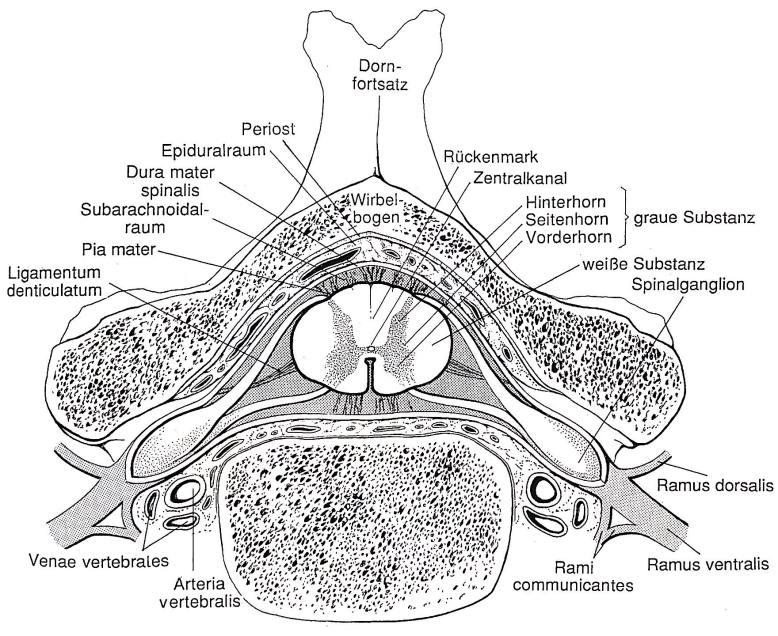
\includegraphics[width=0.8\textwidth]{pictures/Bilder_Jule/Andere/rueckenmark_wirbelsaeule.png}
     \caption[Querschnitt durch Wirbelsäule und Rückenmark]{\textbf{Querschnitt durch Wirbelsäule und Rückenmark.} Aufhängung des Rückenmarks innerhalb der Wirbelsäule eines höheren Primaten. Die dorsale Seite ist nach oben, die ventrale nach unten orientiert. \textsuperscript{\cite[6]{storch2012lehrbuchzoo}}}
     \label{fig:ruckenmark_wirbelsaeule}
\end{figure}


\subsection{Hirnnerven}
\label{subsec:Hirnnnerven}
\index{Hirnnerven !allgemein}
%%%%%%%%%%%%%%%%%%%%%%%%%%%%%%%%%%%%%%%%%%%%%%%%%%%%%%%%%%%
%%%%%%%%%%%%%%%%%%%%%%%%%%%%%%%%%%%%%%%%%%%%%%%%%%%%%%%%%%%

Zwischen dem Gehirn und den peripheren Strukturen verlaufen insgesamt zwölf Hirnnerven. Diese bilateralen, gepaarten Nerven beinhalten sowohl afferente als auch efferente Fasern. Die Nummerierung der Hirnnerven verläuft von rostral nach caudal. Die ersten beiden Hirnnerven liegen am Vorderhirn. Der \textbf{N. olfactorius (I)}\index{Hirnnerven !N. olfactorius} beinhaltet sensorische Fasern, die Information aus dem Riechepithel zum Bulbus olfactorius weiterleiten. Er ist wesentlicher Bestandteil des Geruchssinns. Der zweite Hirnnerv, der \textbf{N. opticus (II)}\index{Hirnnerven !N. opticus} beinhaltet ebenfalls ausschließlich sensorische Fasern. Diese leiten Informationen aus der Retina zum Nucleus geniculatum laterale weiter. Der N. opticus ermöglicht das Sehen und ist zudem am Pupillenreflex beteiligt. Die restlichen Hirnnerven sind am Hirnstamm lokalisiert (Abb.~\ref{fig:hirnnerven_schaf}) \textsuperscript{\cite[10]{crossman2014neuroanatomy}}. \\

\noindent Der \textbf{N. oculomotorius (III)}\index{Hirnnerven !N. oculomotorius} beinhaltet sowohl motorische als auch parasympathische Fasern. Die motorischen Fasern innervieren extraokulare Muskeln, die die Augenbewegungen steuern, wie den superioren, inferioren und medialen Musculus rectus. Der Großteil dieser motorischen Fasern entspringt dem Nucleus oculomotorius, der sich im Mesencephalon etwa auf Höhe des Colliculus superior befindet. Über den N. oculomotorius werden Augenbewegungen gesteuert, sowie das Anheben des oberen Augenlids. Die parasympathischen Fasern des N. oculomotorius erhalten Informationen aus dem Edinger-Westphal Nucleus (\textit{Nucleus accessorius nervi oculomotorii}). Diese Fasern innervieren den Musculus sphincter pupillae, den Ringmuskel des Auges, der die Pupille verengt, sowie den Ziliarmuskel des Auges, der an Augenbewegungen beteiligt ist. Durch diese Verbindung ist der N. oculomotor auch auch an der Pupillenkontraktion und der Pupillenakkommodierung beteiligt. Ähnlich wie der N. opticus ist auch der \textbf{N. trochlearis (IV)}\index{Hirnnerven !N. trochlearis} funktionell für die Augenbewegungen zuständig. Er enthält motorische Fasern, die vom Nucleus trochlearis zum Musculus obliquus superior der äußeren Augenmuskulatur ziehen. Der \textbf{N. trigeminus (V)}\index{Hirnnerven !N. trigeminus} enthält sowohl motorische als auch sensorische Fasern. Die sensorischen Fasern enthalten Informationen aus Gesicht, Kopfhaut, Augenhornhaut, Nasen- und Mundhöhle, sowie der Dura mater des Schädels. Diese Informationen werden zum sensorischen Nucleus des Trigeminus weitergeleitet. Die Funktion des sensorischen fünften Hirnnerven besteht in der Sinneswahrnehmung des Kopfes. Die motorischen Fasern dieses Nervs ziehen von den Motornuclei zu den Musculi masticatorii (Kaumuskulatur) und dem Musculus tensor tympani (Spanner des Trommelfell). Durch diese Projektionen ist der N. trigeminus in das Öffnen und Schließen des Mundes, sowie in die Spannung des Trommelfells involviert. Ein weiterer Hirnnerv, der in die Augenbewegung involviert ist, ist der \textbf{N. abducens (VI)}\index{Hirnnerven !N. abducens}. Er führt motorische Fasern, die vom Nucleus abducens aus dem caudalen Pons zum lateralen Musculus rectus ziehen. Im \textbf{N. facialis (VII)}\index{Hirnnerven !N. facialis} verlaufen sowohl sensorische, motorische und parasympathische Fasern. Die sensorischen Fasern entspringen dem anterior gelegenen Zweidrittel der Zunge und enden im Nucleus solitarius. Diese sensorischen Fasern sind für den Geschmackssinn verantwortlich. 
Ein Teil der motorischen Fasern des Facialis verläuft vom Nucleus facialis zum Musculus stapedius, der am Stapediusreflex beteiligt ist. Dadurch kann die Spannung der Mittelohrmuskulatur reguliert werden. Andere motorische Fasern enden an jenen Muskeln, die für die Mimik zuständig sind.  Die parasympathischen Fasern des N. facialis sind für den Speichel- und Tränenfluss verantwortlich. Sie ziehen vom superioren Nucleus salivatorius zu den Speichel- und Tränendrüsen. Der achte Hirnnerv, der \textbf{N. vestibulocochlearis (VIII)}\index{Hirnnerven !N. vestibulocochlearis} enthält sensorische Fasern. Diese ziehen vom Vestibularorgan und der Cochlea zu den Nuclei vestibularis, bzw. den Nuclei cochlearis. Funktionell ist der N. Vestibulocochlearis für den Gleichgewichts- und Hörsinn verantwortlich. Der \textbf{N. glossopharyngeus (IX)}\index{Hirnnerven !N. glossopharyngeus} beinhaltet sensorische, motorische und parasympathische Fasern. Ein Teil der sensorischen Fasern ist an der allgemeinen Sinneswahrnehmung beteiligt. Sie ziehen aus dem Pharynx, dem posterioren Drittel der Zunge, der Eustachischen Röhre und dem Mittelohr zum sensorischen Nucleus des Trigeminus. Ein weiterer Teil der sensorischen Fasern ist speziell für den Geschmackssinn, Chemorezeption und Druckrezeption verantwortlich. Diese Fasern entspringen unter anderem dem posterioren Drittel der Zunge, sowie dem Sinus caroticus, einer Gefäßerweiterung, die mittels Druckrezeptoren bei der Regulation des Blutdrucks mitwirkt. Die motorischen Fasern des N. glossopharyngeus entspringen dem Nucleus ambiguus und enden im Musculus stylopharyngeus, der für das Schlucken zuständig ist. Ähnlich wie die parasympathischen Fasern des N. facialis sind die parasympathischen Fasern des N. glossopharyngeal ebenfalls am Speichelfluss beteiligt. Sie ziehen vom inferioren Nucleus salivatorius zur Ohrspeicheldrüse (Glandula parotis). Auch der zehnte Hirnnerv, der \textbf{N. vagus (X)}\index{Hirnnerven !N. vagus}, führt alle drei Fasertypen. Die sensorischen Fasern ziehen dabei teilweise, ähnlich wie die Fasern des IX, aus Rachen (Pharynx), Kehlkopf (Larynx), Luftröhre (Trachea), Speiseröhre (Oesophagus) und dem Außenohr zum sensorischen Ncl. des Trigeminus. Diese Fasern sind funktionell in die allgemeine Sinneswahrnehmung involviert. 
Ein anderer Teil der sensorischen Fasern des Vagusnervs entspringt den Eingeweiden in Thorax und Abdomen, dem Glomus aorticum, und dem Aortenbogen (Arcus aortae). Diese sensorischen Fasern enden im Nucleus solitarius und sind für die viszerale Sinneswahrnehmung, bzw. Chemo- und Druckrezeption zuständig. Die motorischen Fasern des N. vagus entspringen dem Ncl. ambiguus und führen wiederum zum Gaumensegel (Velum palatinum), Pharynx, Larynx und oberen Oesophagus. Ihre Funktion besteht im Schlucken und Sprechen. Die im Vagusnerv enthaltenen parasympathischen Fasern verlaufen vom dorsalen Motornucleus des Vagusnervs zu dem thorakalen und abdominalen Eingeweiden. Diese Fasern sind für die Innervation der Herzmuskulatur (Myokard), der Drüsen des Herzkreislaufsystems, sowie der Atemwege und des Magen-Darm-Trakts zuständig. Der \textbf{N. accessorius (XI)}\index{Hirnnerven !N. accessorius} führt ausschließlich motorische Fasern, die den Musculus sternocleidomastoideus ('Kopfnicker') der Halsmuskulatur und den Musculus trapezius der Schultermuskulatur innerviert. Er ist für die Bewegung von Hals und Schultern zuständig. Der N. accessorius weißt eine starke Verbindung zum Rückenmark auf. Der letzte Hirnnerv, der \textbf{N. hypoglossus (XII)}\index{Hirnnerven !N. hypoglossus}, enthält ebenfalls Motorneurone. Diese innervieren, vom Nucleus hypoglossus ausgehend, die innere und äußere Zungenmuskulatur. Dadurch ist er funktionell für die Bewegung der Zunge zuständig \textsuperscript{\cite[10]{crossman2014neuroanatomy}}.

\begin{figure}[H]
    \centering
    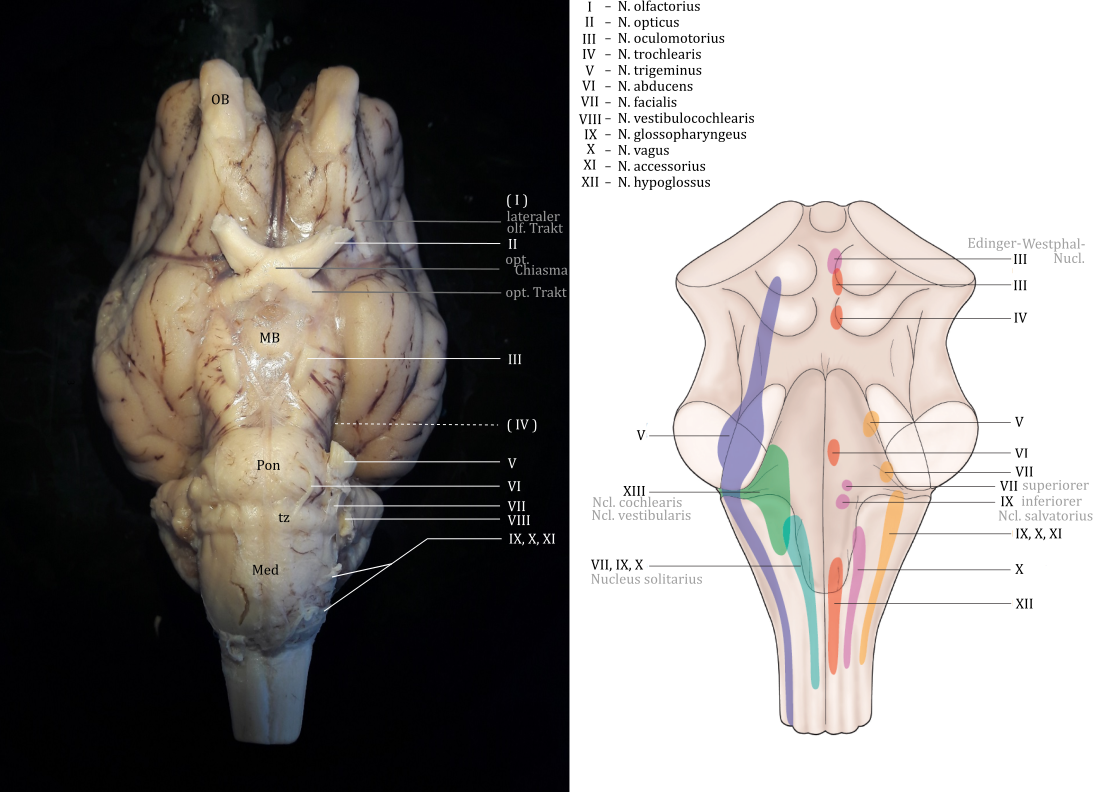
\includegraphics[width=\textwidth]{pictures/Bilder_Jule/Schaf/Aussenansicht/Hirnnerven.png}
    \caption[Hirnnerven Schaf]{\textbf{Hirnnerven Schaf.} \textbf{LINKS:} Ventralansicht des Schafshirn. Gekennzeichnet sind die Hirnnervenkerne. Der Bulbus olfactorius (\textbf{OB}), der Mammillarkörper (\textbf{MB}), der Pons (\textbf{Pon}), der Trapezkörper (\textbf{tz}), sowie die Medulla (\textbf{Med}) sind ebenfalls gekennzeichnet. Da der N. trochlearis nicht sichtbar ist, ist lediglich seine ungefähre Position markiert. \textbf{RECHTS:} dorsale Ansicht des Hirnstamms des Schafs. Markiert sind die Nuclei der Hirnnerven. Dabei sind die sensorischen Kerngebiete links, die motorischen rechts gekennzeichnet \textsuperscript{\cite[10]{crossman2014neuroanatomy}}. \textcolor{red}{BILD am Ende so oben in den Text, dass es passt und der Text nicht so ein großer Block ist...}}
    \label{fig:hirnnerven_schaf}
\end{figure}{}


\subsection{Externe Merkmale des Gehirns}
\label{subsec:Externe_Merkmale}
%%%%%%%%%%%%%%%%%%%%%%%%%%%%%%%%%%%%%%%%%%%%%%%%%%%%%%%%%%%
%%%%%%%%%%%%%%%%%%%%%%%%%%%%%%%%%%%%%%%%%%%%%%%%%%%%%%%%%%%

\subsubsection{Hirnhäute} \index{Hirnhäute}
%%%%%%%%%%%%%%%%%%%%%%%%%%%%%%%%%%%%%%%%%%%%%%%%%%%%%%%%%%%

Drei Hirnhäute liegen zwischen dem Gehirn und dem Schädelknochen (Abb.~\ref{fig:hirnhaeute}). Die äußerste Schicht ist die Dura mater, auch harte Hirnhaut genannt. Sie ist lederartig, unelatisch und fest und umgibt schützend sowohl Gehirn als auch Rückenmark. Die spinnennetzartige Arachnoidae mater encephali oder auch Spinnenhaut, befindet sich dirket unter der Dura mater. Die unterste Schicht bildet die Pia mater, auch weiche Hirnhaut genannt. Diese dünne Haut schmiegt sich eng an die Oberfläche des Gehirns an. "Entlang der Pia mater verlaufen viele Blutgefäße, die schließlich ins darunterliegende Gehirn führen" \textsuperscript{\cite[7]{neurowissenschaften_baer}}. Zwischen der Arachnoidea und der Pia mater befindet sich der Subarachnoidalraum. Dieser ist mit Liquor cerebrospinalis\index{Liquor cerebrospinalis}. In dieser dünnen Schicht aus farbloser Flüssigkeit schwimmt das Gehirn innerhalb des Schädels \textsuperscript{\cite[7]{neurowissenschaften_baer}}.

\begin{figure}[H]
	\centering
	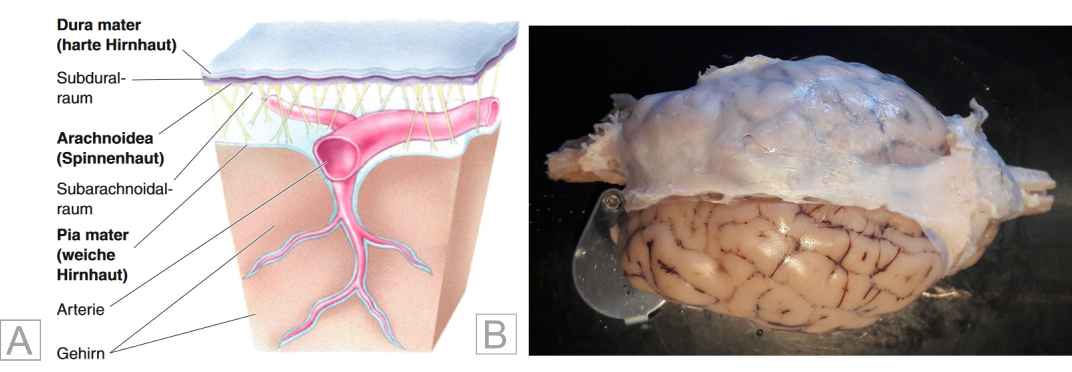
\includegraphics[width=\textwidth]{pictures/Bilder_Jule/Andere/hirnhaeute2.png}
	\caption[Die Hirnhäute]{\textbf{Die Hirnhäute.} \textbf{A}: Anordnung der drei Hirnhäute als Schema. \textbf{B}: Veranschaulichung der Hirnhäute am Schafhirn. Über der linken Hemisphäre ist die Dura mater zu sehen. Auf der linken Hemisphäre ist die Pia mater zu sehen. Die Dura mater Arachnoidea wurde von dieser Hälfte inklusive Arachnoidea entfernt.}
	\label{fig:hirnhaeute}
\end{figure}


\subsubsection{Anhängende Strukturen}
\label{subsubsec:Hirnanhangsstrukturen}
%%%%%%%%%%%%%%%%%%%%%%%%%%%%%%%%%%%%%%%%%%%%%%%%%%%%%%%%%%%

\subsubsection*{Riechepithelium} \index{Riechepithel}
%%%%%%%%%%%%%%%%%%%%%%%%%%%%%%%%%%%%%%%%%%%%%%%%%%%%%%%%%%%%

Das Riechepithelium befindet sich außerhalb des Gehirns und ist am rostralen Ende mit diesem Verbunden. Es kleidet als Anteil der Nasenschleimhaut die obere Nasenmuschel und die gegenüberliegende Nasenscheidewand aus und überdeckt  ein  System aus Strömungskörpern (Abb.~\ref{fig:Riechepithel}). Das Riechepithel stellt die erste Station der Riechbahn dar \textcolor{red}{(VERWEIS: Riechsinn)}. In diesem mehrschichtigen Sinnesepithel sind die chemorezeptiven Riechsinneszellen lokalisiert. Die axonalen Fortsätze dieser Zellen ziehen bis in die vordere Schädelgrube, wo sich der Bulbus olfactorius\index{Bulbus olfactorius} befindet. Bei Spezies mit gutem Riechvermögen nehmen Riechepithel und Bulbus olfactorius mehr Platz ein als bei Tieren, für deren Lebensweise der Riechsinn verhältnismäßig weniger relevant ist, wie beispielsweise bei Menschenaffen.

\begin{figure}[H]
    \centering
    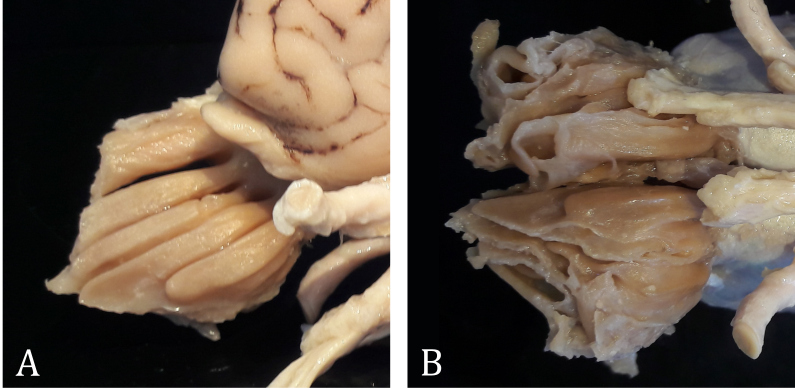
\includegraphics[width=0.8\textwidth]{pictures/Bilder_Jule/Schaf/Ausschnitte/Riechepithel.png}
    \caption[Riechepithelium Schaf]{\textbf{Riechepithelium Schaf}. Mediale \textbf{A} und inferiore \textbf{B} Ansicht des Riechepitheliums des Schafes.}
    \label{fig:Riechepithel}
\end{figure}{}


\subsubsection*{Hypophyse}
\label{subsubsec:hypophyse} \index{Hypophyse !allgemein}
%%%%%%%%%%%%%%%%%%%%%%%%%%%%%%%%%%%%%%%%%%%%%%%%%%%%%%%%%%%%

Die Hypophyse liegt inferior, leicht caudal des Chiamsa opticums und rostral des Mammillarkörpers. Über den Hypophysenstiel (Infundibulum) ist hängt sie am Hypothalamus 

\begin{wrapfigure}{r}{0.38\textwidth}
    \centering
    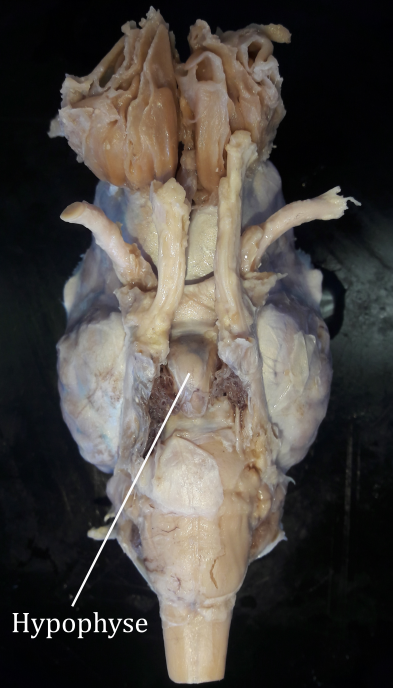
\includegraphics[width=0.35\textwidth]{pictures/Bilder_Jule/Schaf/Aussenansicht/Hypophyse.png}
    \caption[Hypophyse Schaf.]{\textbf{Hypophyse Schaf.}}
    \label{fig:hypophyse}
\end{wrapfigure}

\noindent (Abb.~\ref{fig:hypophyse}) \textsuperscript{\cite[4]{trepel2011neuroanatomie}}. Die Hypophyse besteht aus zwei Teilgebieten: der Neurohypophyse\index{Hypophyse !Neurohypophyse} und der Adenohypophyse\index{Hypophyse !Adenohypophyse}. Dabei ist lediglich die \textbf{Neurohypophyse} (Hypophysenhinterlappen) Teil des Diencephalons. Die Neurohypophyse besitzt keine dichte Blut-Hirn-Schranke, somit können Hormone, die von den dort lokalisierten Nervenzellen sezerniert werden, via Neurosekretion ins Blut gelangen. Die deutlich größere \textbf{Adenohypophyse} (Hypophysenvorderlappen) umhüllt den kleineren Hypophysenhinterlappen teilweise. Sie ist kein Bestandteil des Gehirns, sie ist lediglich an das Diencephalon angelagert. Somit besteht die Adenohypophyse nicht aus Nervengewebe, sondern aus Drüsenepithel. Durch die dort gebildeten glandotropen Hormone kann die Adenohypophyse auf endokrine Drüsen, wie die Schilddrüse oder die Nebennierenrinde, wirken. Diese Drüsen nehmen dann durch die Produktion eigener Hormone  Einfluss auf periphere Organe. Auch Effektorhormone werden in der Adenohypophyse gebildet. Diese können dirket, ohne Zwischenschaltung weiterer Drüsen, auf periphere Organe wirken. Die Hormone der Adenohypophyse sind unter anderem an der Pigmentierung der Haut, an der Milchbildung in der Brustdrüse, am Körperwachstum und an der Reifung von Ei- und Spermienzellen beteiligt. Generell ist die Hypophyse als das hormonelle 'Ausführungsorgan' des Hypothalamus\index{Hypothalamus} zu betrachten (Kap.~\ref{subsubsec:Hypothalamus}) \textsuperscript{\cite[8]{trepel2011neuroanatomie}}.

%%%%%%%%%%%%%%%%%%%%%%%%%%%%%%%%%%%%%%%%%%%%%%%%%%%%%%%%%%%%%
%%%%%%%%%%%%%%%%%%%%%%%%%%%%%%%%%%%%%%%%%%%%%%%%%%%%%%%%%%%%%
% Allgemeine sensorische Bahnen
\newpage
\section{Allgemeine sensorische Bahnen}
Dieses Kapitel behandelt die allgemeine Sensorik \index{Sensorik !allgemein} die im Gegensatz zu speziellen Sensorik (Kapitel~ \ref{sec:spezsens}) steht. In der allgemeine Sensorik sind die Sinne zusammen gefasst welche über den ganzen Körper verteilt sind, dazu gehören unter anderem die Somatosensorik \index{Sensorik !Somato-} die Propriozeption \index{Propriozeption} und die Viszerosensorik \index{Sensorik !Viszero-}\textsuperscript{\cite[22]{kandel2013principles}}. Die spezielle Sensorik \index{Sensorik !speziell} fasst die Sinne zusammen welche auf Grund der Cephalisation bei Säugern nach vorne in den Kopf verlagert sind.
\\
\noindent
Die Somatosensorik zeichnet sich durch die Repräsentation der direkten äußeren Welt und der inneren Welt aus. Bei der Repräsentation der Außenwelt unterscheidet man bei Säugetieren zwischen zwei Rezeptorsystemen. Zum einen die haarlose Haut in den Handinnenflächen, an der Fußunterseite und an den Lippen und der Nase, zum anderen die behaarte Haut mit hoch spezialisierten Tastsinneszellen innerviert durch die Bewegungen des Follikels auf den Blutsinus \index{Blutsinus} der Vibrissen.  \index{Sinushaar} \textsuperscript{\cite[24]{paxinos2014rat}}
Die Propriozeption codiert die Informationen der relative Position unserer Extremitäten und anderer Körperteile im Raum und bildet in den Vorderextremitäten die Grundlage für abstrakte Wahrnehmung von Objektgrößen und Gewicht. Ein weiteren Bereich in der Somatosensorik bildet der Sinn welcher Schmerzen und Temperatur verarbeitet. \textsuperscript{\cite[24]{paxinos2014rat}}
Im Weiteren wird am Beispiel der Ratte näher auf die unterschiedlichen Systeme eingegangen und wodurch diese sich genau unterscheiden. 


% Somatosensorik
\subsection{Somatosensorik \index{Somatosensorik} des Körpers}
Die Somatosensorik des Körpers wird in zwei Systeme unterteilt, wobei der Tastsinn \index{Tastsinn} und die Propriozeption das lemniskale System \index{System !lemniskal} bilden und der Schmerz- und Temperatursinn  das anterolaterales System. \index{System !anterolateral} Beide Systeme werden durch die Rezeptoren unter der haarlosen Haut der Säuger innerviert.

\subsubsection{Tastsinn und Propriozeption (lemniskales System)}

\subsubsection*{Rezeptoren}
Die Rezeptoren des lemniskalen Systems werden unterteilt, in ihre Lage unter der Haut und ihre Adaptationseigenschaften. Dadurch unterscheiden sie sich in der Modalität, die sie codieren. Bei der Lage wird unterschieden zwischen direkt unter der Oberfläche oder tiefer im Gewebe liegenden Nervenendigungen und schnell bzw. phasisch und langsam bzw. phasisch-tonisch Adaptation dieser Nerven.\\
Direkt unter der Hautoberfläche liegen die Meissner- und die Merkel-Rezeptoren welche für Bewegung und Druck sowie in abstrakterem Sinne für Form, Textur und das Greifen nach Objekten codieren. \textsuperscript{\cite[24]{paxinos2014rat}} Tiefer unter der Haut liegen die Pacini-Rezeptoren welche schnell adaptierende Rezeptoren sind, die für Vibrationen codieren. Zusammen mit den Meissner- und Merkelrezeptoren bilden sie den bewussten Tastsinn. Die Neurone der Rezeptoren sind dicke, myelinisierte A$\alpha$ Nervenfasern mit einer Leitgeschwindigkeit von 72-120 m/s \textsuperscript{\cite[22]{kandel2013principles}}. Unbewusst werden von den langsamen, tief unter der Haut liegenden Ruffini-Rezeptoren Informationen über die Dehnung der Haut und der Muskeln, damit der Position der Gelenke und Extremitäten weiter gegeben.
Die Nervenfasern der Propriozeption sind dicke, myelinisierte A$\beta$ Nerven deren Durchmesser etwas geringer ist als, der der A$\alpha$ Neuronen.
Die Nervenfasern eines Hautgebiets werden zu einem peripheren Nervenstrang gebündelt und ziehen in das Spinalganglion innerhalb des Wirbelkanals. Die Zellkörper der Nervenfasern liegen in diesem Spinalganglion und sind umgeben von speziellen Gliazellen. Zwischen den Nervenzellen verlaufen fenstrierte Kapillaren und versorgen die Nervenfasern mit den nötigen Nährstoffen. 

\subsubsection*{Rückenmark}
Die Axone der Nerven ziehen weiter in die Wirbelsäule. Da hier keine synaptische Verschaltung statt findet, ziehen die Axone direkt in die weiße Substanz des Rückenmarks und steigen parallel zum Verlauf der Wirbelsäule auf. Die Axone unterhalb des sechsten thorakalen Segments (T6) bilden den \textit{Fasciculus gracilis} \index{Fasciculus !gracilis} und die Axone oberhalb des sechsten Thorakalsegments (T6) formen den \textit{Fasciculus cuneatus} \index{Fasciculus !cueatus} im dorsalen Teil der weißen Substanz des Rückenmarks (Abb.~\ref{fig:bahnen_rueckenmark}) \textsuperscript{\cite[8]{paxinos2014rat}}. F.~gracilis und F.~cuneatus bilden somit die wichtigste aufsteigende Bahn für die sensorischen Informationen aus dem Tastsinn und der Eigenwahrnehmung hinauf in den Hirnstamm. 
Die Trennung zwischen F.~gracilis und F.~cuneatus ist wichtig, da die sie in zwei anatomisch unterschiedlichen Kernen des Hirnstamms terminieren. Sie bilden zusammen mit anderen kleineren Bahnen den Hinterstrang (eng.: dorsal column) \textsuperscript{\cite[22]{kandel2013principles}}. 

\begin{figure}[H]
    \centering
    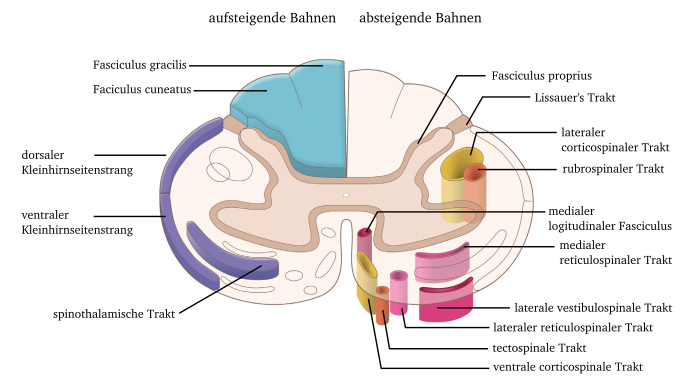
\includegraphics [width = \textwidth]
    {pictures/somatosensory/aufabsteigendeBahnen_Rueckenmark.png}
    \caption[Auf- und Absteigende Bahnen im Rückenmark]{\textbf{Auf- und Absteigende Bahnen im Rückenmark}\\ Zur besseren Veranschaulichung der Bahnen sind die Bahnen in der Abbildung nach absteigenden Bahnen auf der linken Seite und absteigenden Bahnen auf der rechten Seite aufgeteilt. Beide Gruppen kommen jeweils gespiegelt auch auf der anderen Seite vor.
    \textsuperscript{\cite[8]{crossman2014neuroanatomy}}}
    \label{fig:bahnen_rueckenmark}
\end{figure}

\subsubsection*{Nucleus gracilis und Nucleus cuneatus - Medulla}

Die Axone des \textit{Fasciculus~gracilis} terminieren im \textit{Nucleus~gracilis} in der Medulla. Auf gleicher Ebene der Medulla enden auch die Axone des \textit{Fasciculus~cuneatus} im \textit{Nucleus~cuneatus}. Zusammen werden die beiden Kerne auch Hinterstrangkerne oder im englischen dorsal column nuclei genannt. in Abbildung~\ref{fig:nucleus_cuneatus} kann man den Nucleus~cuneatus (gelb) sehen. Der Nucleus liegt dorsal des Kerngebiets des Trigeminusnervs (Sp5I) und lateral des vierten Ventrikels (4V). Die Abbildung zeigt nicht den Nucleus gracilis.
\\
\noindent
Beide Nuclei sind zylindrisch geformt und in rostrocaudaler Richtung ausgedehnt. Die afferenten Neuronen aus einer Hautregion enden in der rostrocaudalen Ausdehnung auf einer Linie und verschiedene Hautregionen werden lateral-medial repräsentiert. Die somatosensorische Repräsentation auf dieser Ebene gleicht einem auf dem Rücken liegenden, kopflosen Homunculus. Dabei liegen die distalen Körperregionen lateral und die proximalen Hautregionen medial in den Nuclei. Die taktilen und propriozeptiven Informationen des Kopfes (Kap.~\ref{sec:somatokopf}) werden in angrenzenden \textit{Nucleus principalis nervi trigemini} repräsentiert \textsuperscript{\cite[22]{kandel2013principles}}. 
\\
\begin{figure}[H]
    \centering
    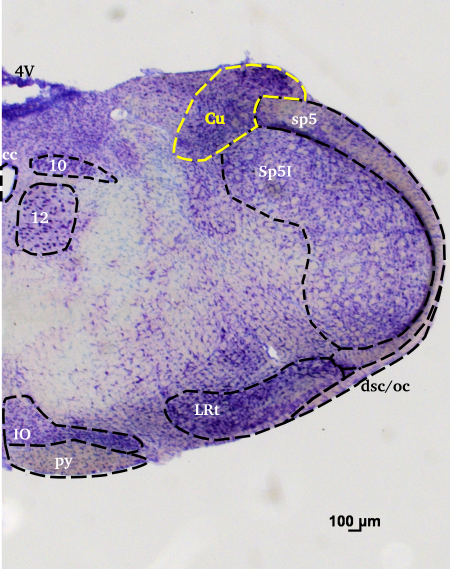
\includegraphics{pictures/somatosensory/nucleus_cuneatus.png}
    \caption[Lage des \textit{Nucleus cuneatus} in der Medulla]{\textbf{Lage des \textit{Nucleus cuneatus} in der Medulla}\\
    Nissel-Färbung der Rattenhirns auf der Höhe der Medulla (N02\_3R). Der Ausschnitt zeigt die rechte Seite vom Zentralkanal (cc) bis zum Trigeminusnerv (sp5). Oberhalb des Kerngebiets des Trigeminusnervs (SP5I) liegt der Nucleus~cuneatus (Cu). Die Schnittebene beinhaltet sowohl Teile der Medulla, daran zu erkennen, dass der vierter Ventrikel (4V) angeschnitten ist, als auch Teile des Rückenmarks, daran zu erkennen, dass der Zentralkanal (cc) zu sehen ist. Weitere Kerngebiete sind: der dorsaler Kern des Nervus vagus(10), Kern des Nervus hypoglossus (12), die untere Olive (IO) und der Nucleus reticularis lateralis (LRt). Ebenfalls zu sehen sind: die Pyramidenbahn (py), der dorsaler spinocerebellarer Tract/olivocerebraler Tract (dsc/oc) und der Trigeminusnerv (sp5).}
    \label{fig:nucleus_cuneatus}
\end{figure}

\subsubsection*{Der Mediale Lemniscus}
In den Hinterstrangkernen ist die erste synaptische Verbindung im lemniskalen System. Von den primär afferenten Axonen aus dem Rückenmark wird das Signal an die Nervenfasern des \textit{medialen~Lemniscus} weiter geleitet. Diese kreuzen die Mittellinie auf der Höhe der Medulla und verlaufen anschließend contralateral \textsuperscript{\cite[22]{kandel2013principles}}. 
Der \textit{mediale~Lemniscus} liegt ventral-medial in der Medulla und zieht von der Medulla bis in den Thalamus im Diencephalon. Die Veränderung der Lage des \textit{medialen~Lemniscus} \index{medialer Lemniscus} kann man in Abbildung \ref{fig:medialer_lemniscus} verfolgen. Er beginnt schon auf der Höhe des Nucleus cuneatus (Abb.~\ref{fig:somato_pathway}) und zieht sich dann ventral-medial unterhalb des Aqueduct (Abb.~\ref{fig:medialer_lemniscus}A) weiter nach rostral. Dabei verändert er seine Lage in sofern, dass er von ventral-medial nach medial-lateral (Abb.~\ref{fig:medialer_lemniscus}B) zieht. Der mediale~Lemniscus zieht sich auf der Höhe des dritten Ventrikels (Abb.~\ref{fig:medialer_lemniscus}C) zentral im Diencephalon bis in den Thalamus.

\begin{figure}[H]
    \centering
    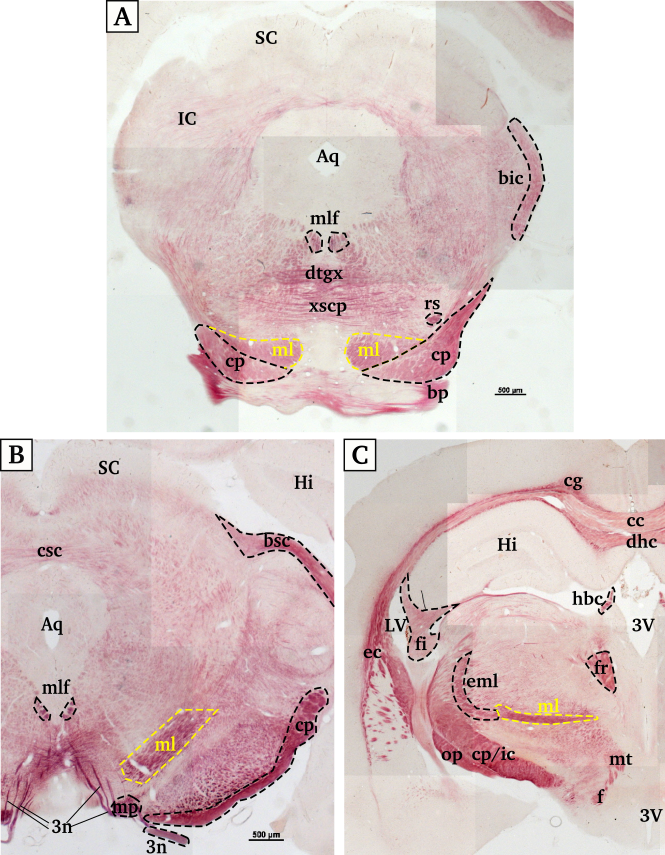
\includegraphics[width = 0.9\textwidth] {pictures/somatosensory/medial_lemniscus.png}
    \caption[Verlauf des \textit{medialen Lemniscus}]{\small{\textbf{Verlauf des \textit{medialen Lemniscus}}\\
    Faserschnitte auf der Höhe des Mesencephalons (A \& B) und des Diencephalons (C). Man kann den Verlauf des medialen Lemniscus in der Schnittserie über 3450~$\mu$m verfolgen.\\
    \textbf{A} (F14\_4P): Colliculus superior (SC), Colliculus inferior (IC), Aqueduct (Aq), Brachium des IC (bic), brachia pontis (bp, eng.: middle cerebellar peduncle), Großhirnstiele (Pedunculi cerebri) (cp), dorsal tegmental decussation (dtgx), Fasciculus longitudinalis medialis (mlf), rubrospinaler tract (rs), decussation des SC peduncels (xscp).
    \textbf{B} (F17\_3P): Nervus oculomotorius (3n), Hippocampus (Hi), Brachium des SC (bsc), Kommissur des SC (csc), mammillary peduncle (mp).
    \textbf{C} (F20\_3P): dritter Ventrikel (3V), lateraler Ventrikel (LV), zentrale Kommissur (cc), cingulum (cg), dorsale Hippocampuskommissur (dhc), Capsula externa (ec), external medullary lamina (eml), Fornix (f), Fimbria (fi), fasciculus retroflexus (fr), Commissura habenularum (hbc), Kapsula interna (ic), mammillothalamic tract (mt), optischer tract (op)}}
    \label{fig:medialer_lemniscus}
\end{figure}

\subsubsection*{Thalamus}
Die Informationen aus den Hautschichten von den Meissner-, Merkel- und Pacini-Rezeptoren, die über den die primär afferenten Neuronen und den \textit{medialen Lemniscus} kommen, werden im lateralen und medialen Nucleus ventralis posterior (eng.: lateral and medial
ventral posterior nuclei) verarbeitet. Proprioceptive Informationen aus den Gelenken und dem Bauchraum werden über den medialen Lemniscus an den oberen Nucleus ventralis posterior (eng.: superior ventral posterior nucleus) weitergeleitet \textsuperscript{\cite[22]{kandel2013principles}}. 
In der Nisselfärbung des Rattenhirns ist keine Abgrenzung der einzelnen Nuclei des Thalamus sichtbar. Der Thalamus als Verschaltungszentrale des Diencephalons liegt bei der Ratte zentral unter dem dritten Ventrikel (3V, Abb.~\ref{fig:thalamus_somato}) und oberhalb des Hypothalamus. 
Am Beispiel des Menschen werden in Kapitel \label{subsubsec:thalamus} die einzelnen Kerne im Thalamus gezeigt, wobei die Lage der somatosensorischen Kerne gut in Abbildung \ref{fig:thalamus_nuclei}~A~\&~B zu sehen ist.
Die zweite synaptische Verschaltung im Thalamus gibt die Informationen an die Neuronen der thalamisch-corticalen Verbindung weiter, welche die Informationen dann an den primären somatosensorischen Cortex leitet.

\begin{figure}[H]
    \centering
    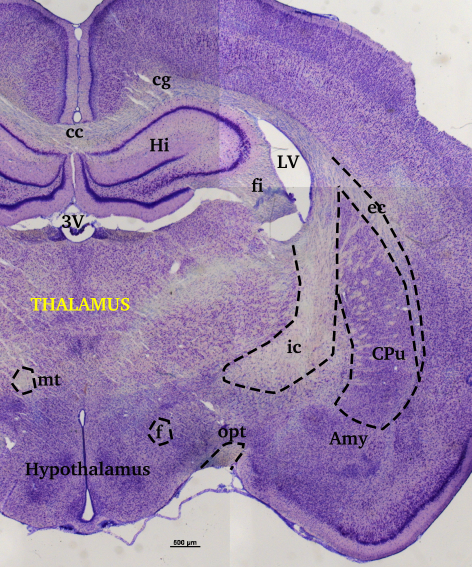
\includegraphics{pictures/somatosensory/thalamus_somato.png}
    \caption[Thalamus]{\textbf{Thalamus}\\
    rechte Gehirnhälfte (N23\_3P) der Ratte auf der Höhe des Thalamus und des dritten Ventrikels (3V). Auf der selben Höhe in Schnitt sind als prominente Hirnstrukturen der Hippocampus (Hi), der Hypothalamus und die zentrale Kommisur (eng.: corpus callosum, cc) zu sehen. Weitere Strukturen sind: der Cortex, Amygdala (Amy), Caudate Putamen (CPu), Cingulum (cg), äußere Kapsel (ec), Fornix (f), Fimbria (fi), innere Kapsel (ic), laterale Ventrikel (LV), mammillothalamic tract (mt), optische Bahn (opt)}
    \label{fig:thalamus_somato}
\end{figure}

\subsubsection*{Primärer Somatosensorischer Cortex}
\label{subsubsec:S1}
Der somatosensorische Cortex liegt beim Menschen auf dem postzentralen Gyrus, direkt hinter dem \textit{Sulcus centralis}. Der primäre somatosensorische Cortex (S1) setzt sich aus den Brodmann-Arealen 3a, 3b, 1 und 2 zusammen und endet anterior im Sulcus centralis und grenzt dort an den primären Motorcortex (Brodmann-Areal 4). Posterior des S1 liegt der posterior Parietalcortex mit den Brodmann-Arealen 5 und 7. In Abbildung \ref{fig:S1_Cortex} ist ein horizontal Schnitt durch die verschiedenen Areale des primären somatosensorischen Cortex und den angrenzenden Strukturen zu sehen \textsuperscript{\cite[23]{kandel2013principles}}. 

\begin{figure}[H]
    \centering
    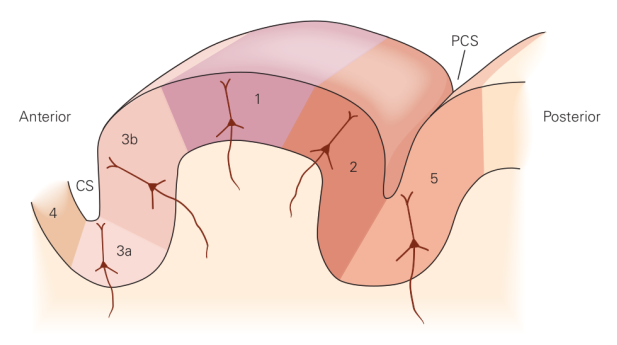
\includegraphics{pictures/somatosensory/S1_Cortex.png}
    \caption[Primärer Somatosensorischer Cortex]{\textbf{Primärer Somatosensorischer Cortex (S1)}\\
    Der primäre somatosensorische Cortex (S1) setzt sich aus den Brodmann-Arealen 3a, 3b, 1 und 2 zusammen und endet anterior im Sulcus centralis (CS) und grenzt dort an den primären Motorcortex (Brodmann-Areal 4). Posterior des S1 liegt der posterior Parietalcortex mit den Brodmann-Arealen 5 und 7 er grenzt sich vom postzentralen Gyrus durch den postzentralen Sulcus (PCS) ab.
    \textsuperscript{\cite[23]{kandel2013principles}}}
    \label{fig:S1_Cortex}
\end{figure}

Betrachtet man den somatosensorischen Cortex in seiner Ausdehnung entlang des Sulcus centralis, wie auch die Schnittebene in Abbildung~\ref{fig:somato_pathway} verläuft, wird nochmal die Somatotopie deutlich. Hierbei ist vor allem der Unterschied zwischen den Tieren sehr prominent. Die somatosensorischen Informationen auf der Hautoberfläche unterscheiden sich in ihrer Größe der rezeptiven Felder und in ihrer daraus resultierenden Relevanz. Auf Grund dessen werden einige Körperregionen mehr repräsentiert als andere eine Darstellung dieser Überrepräsenation ist der Homunculus (Abb.~\ref{fig:somato_homunculus}). Der Homunculus der Ratte ähnelt der des Hasens. 
\\

\begin{figure}[H]
    \centering
    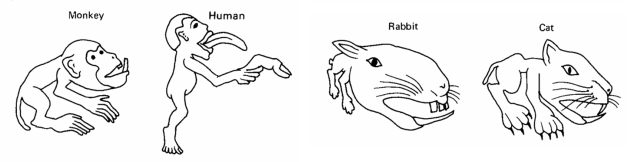
\includegraphics[width = \textwidth] {pictures/somatosensory/homunculus.png}
    \caption[Homunculus]{\textbf{Homunculus}\\
    Homunculi vom Affe (oben links), Menschen (oben rechts), Hase (unten links) und von der Katze (unten rechts).}
    \label{fig:somato_homunculus}
\end{figure}

\newpage
Areal~3b bekommt die Informationen aus den bewussten Mechanorezeptoren der Haut. In diesem Cortexareal werden vor allem die Wahrnehmung der taktilen Reize und deren Form und Textur verarbeitet, wogegen in Areal~3a die Wahrnehmung aus der Körperhaltung und der Proprioception verarbeitet wird. Areal~1 und 2 erhalten ihre Informationen aus Areal~3b. In Areal~1 werden die Informationen aus der strukturellen Beschaffenheit des Objekts weiterverarbeitet und in Areal~2 diese über die Größe und Gestalt. Alle vier Areale des primären somatosensorischen Cortex projizieren in den sekundären somatosensorischen Cortex (S2) \textsuperscript{\cite[12]{neurowissenschaften_baer}}.
\\
\noindent Der sekundäre somatosensorische Cortex liegt unterhalb des primären somatosensorischen Cortex und ist für die Verarbeitung der Informationen aus beiden S1 zuständig. Über den Corpus callosum erhält er die Informationen aus der jeweils anderen Hirnhälfte. Er verarbeitet die bilateralen rezeptiven Felder und ist für den Lerntransfer zwischen den Seiten zuständig. Der S2 ist auch für die generelle Aufmerksamkeit bezüglich taktiler Informationen zuständig \textsuperscript{\cite[12]{neurowissenschaften_baer}}.

Im Gegensatz zu der Lage des somatosensorischen Cortex beim Menschen, steht die Lage bei der Ratte. Da Ratten ein lisencephales Gehirn besitzen und bei diesen Tieren auch kein Sulcus centralis ausgebildet ist, ist die Lokalisation des Areals nicht anhand dessen zu bestimmen. Anhand der Schichtung und Färbungen wurde der somatosensorische Cortex bei der Ratte identifiziert (Abb.~\ref{fig:S1_Cortex_Ratte}). Die Neuronen in dem Teil des Cortex (anterior parietal region) wurden durch eine stark ausgeprägte granuläre Schicht IV und der stärksten Myelinisierung aller Cortexareale identifiziert. \textsuperscript{\cite[22]{paxinos2014rat}}
\\
\begin{figure}[H]
    \centering
    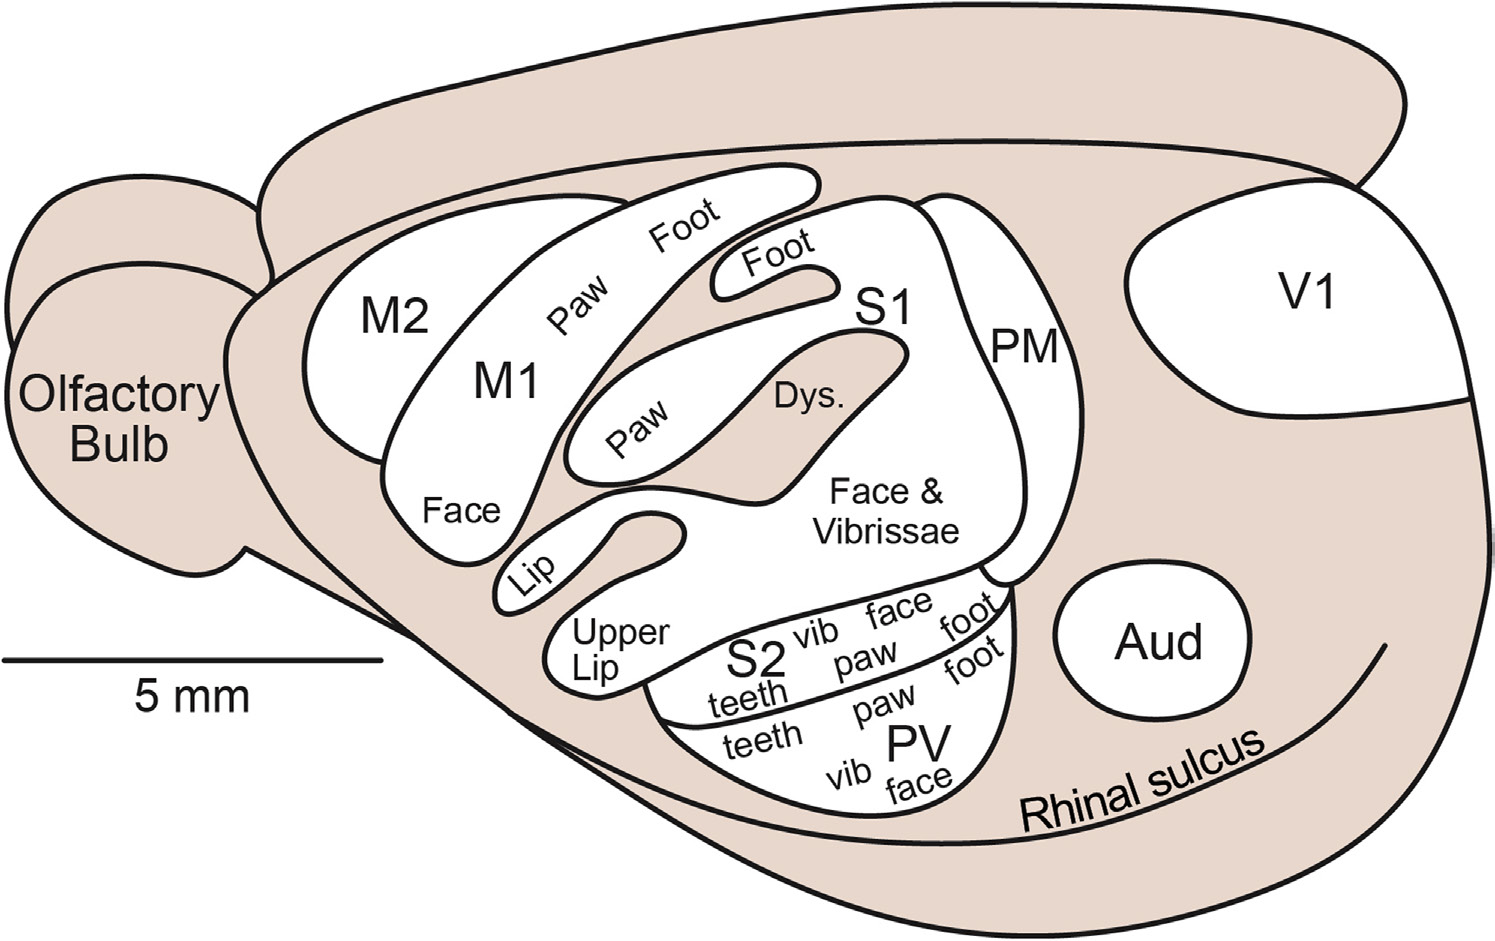
\includegraphics[width = 0.8\textwidth] {pictures/somatosensory/Somato_cortex_ratte.png}
    \caption[Somatosensorischer Cortex der Ratte]{\textbf{Somatosensorischer Cortex der Ratte}\\
    primärer (S1) und sekundärer (S2) somatosensorischer Cortex mit der Repräsentation der einzelnen Körperregionen. Außerdem ist die \textit{Fissura rhinalis} (rhinal sulcus) gezeigt welche den Neocortex vom Archicortex trennt. Anterior vom somatosensorischen Cortex ist der Motorcortex mit primären (M1) und sekundärem (M2) Motorcortex. Ventral des S2 liegt das parietal ventral somatosensorische Areal (PV) und posterior das posteriore mediale Areal (PM). Als Reverenz sind noch der Auditorische Cortex (Aud) und der Visuelle Cortex (V1) gezeigt. \textsuperscript{\cite[24]{paxinos2014rat}}}
    \label{fig:S1_Cortex_Ratte}
\end{figure}

\subsubsection*{Somatosensorische Bahnen}

\begin{figure}[H]
    \centering
    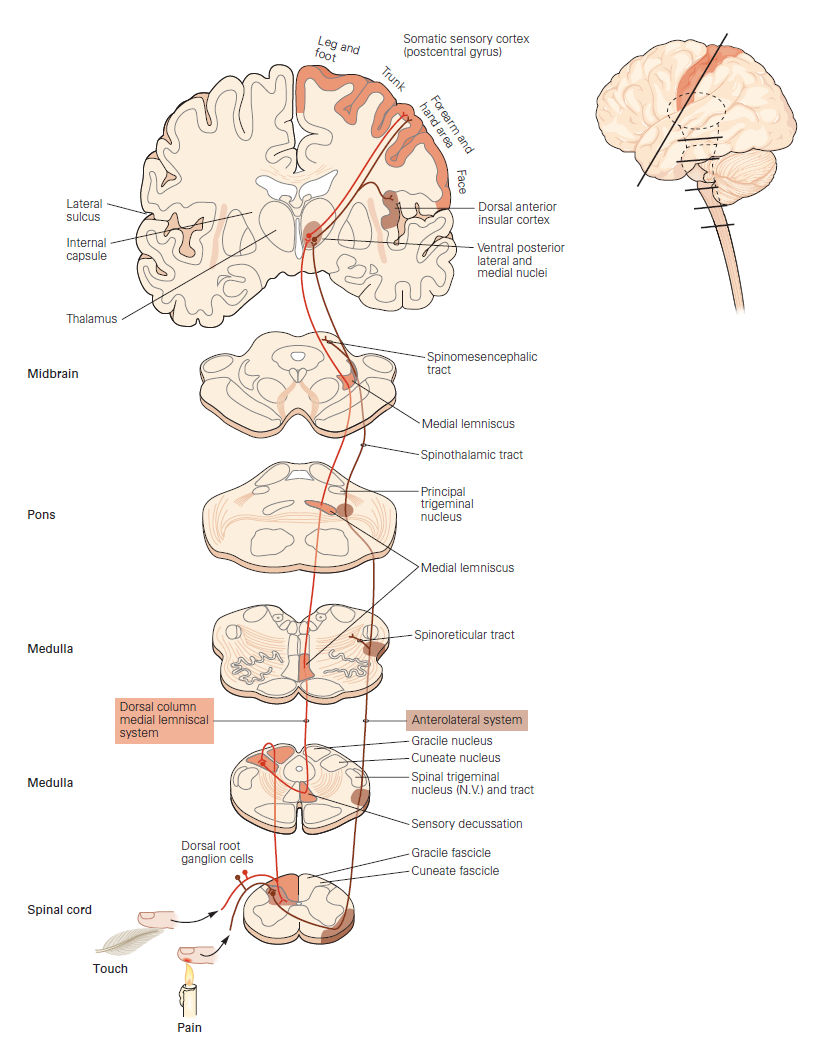
\includegraphics{pictures/somatosensory/pathway_somatosensory2.png}
    \caption[Aufsteigende Bahnen der Somatosensorik]{\textbf{Aufsteigende Bahnen der Somatosensorik}\\
    Die aufsteigenden Bahnen der Somatosensorik sind getrennt in das lemniskale (rot) und das anterolaterale (braun) System. Beginnend im Rückenmark bis zu zum primären somatosensorischen Cortex posterior vom \textit{Sulcus centralis}. Die Bahnen sind am Beispiel des Menschen schematisch dargestellt und sind auf den Ebenen des Rückenmarks, der Medulla, der Pons, des Mittelhirns und des Cortex zu verfolgen.
    \textsuperscript{\cite[22]{kandel2013principles}}}
    \label{fig:somato_pathway}
\end{figure}

\newpage    
\subsubsection{Schmerz und Temperatursinn (anterolaterales System)}
Der Schmerz- und Temperatursinn hat vor allem eine schützende Funktion auf unseren Körper. Er warnt uns vor Verletzungen oder zu großer Hitze, worauf wir dann reflexartig reagieren und zurückweichen oder die Verletzung behandeln. Der Schmerz \textcolor{red}{entspringt} von den somatosensorischen Strukturen in der Haut und wird von dort zu den höheren Gehirnarealen weitergeleitet. 

\subsubsection*{Rückenmark}

Die meisten der Nozizeptoren sind einfache Nervenendigungen primärer sensorischer Faser und können generell in drei Gruppen eingeteilt werden, die thermischen, mechanischen und polymodalen Nozizeptoren \textsuperscript{\cite[24]{kandel2013principles}}. Auch die Zellkörper der Nozizeptoren des Körpers liegen im dorsalen Wurzelganglion und terminieren im Hinterhorn des jeweiligen Segments. Ihre Synapsen konzentrieren sich in den Schichten I, IV, V, VII, und X des Hinterhorns (Abb.~\ref{fig:graymatter}) \textsuperscript{\cite[25]{paxinos2014rat}}.
\\
\\

\begin{figure}[H]
        \centering
        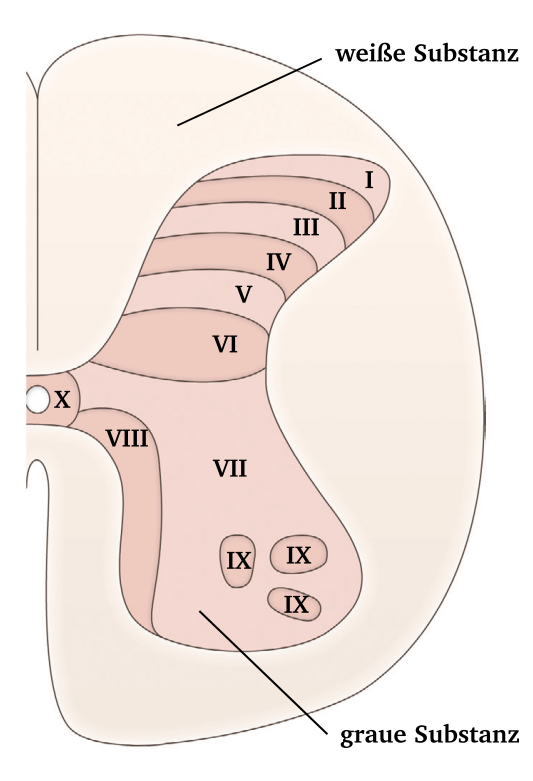
\includegraphics[width = 0.5\textwidth]
        {pictures/somatosensory/gray_matter.png}
        \caption[Schichten in der grauen Substanz des Rückenmarks]{\textbf{Schichten in der grauen Substanz des Rückenmarks} Die Abbildung zeigt schematisch die rechte Seite des Rückenmarks mit weißer und grauer Substanz. Die Schichten der grauen Substanz beginnen im Hinterhorn mit Schicht I und gehen bis Schicht VIII im Vorderhirn. Die Schicht XI liegt in Schicht VIII und Schicht X umgibt den Zentralkanal.
        \cite[8]{crossman2014neuroanatomy}}
        \label{fig:graymatter}
    \end{figure}

\newpage
Diese synaptische Verbindung verbindet die Nozizeptoren mit den spinothalamischen Neuronen. Wie der Name dieser Neuronen schon sagt ziehen die Neuronen vom Rückenmark bis in den Thalamus. Die Zellkörper der Neurone liegen in der grauen Substanz des Rückenmarks, während die Axone in der weißen Substanz des Rückenmarks parallel zum Verlauf der Wirbelsäule in Bahnen auf- und absteigen. Die Axone der spinothalamischen Zellen kreuzen auf der Ebene der ersten Synapse die Mittellinie und steigen in der contralateralen weißen Substanz zum lateralen Bereich des Thalamus auf \textsuperscript{\cite[25]{paxinos2014rat}}. Bei Ratten bildet die größte Gruppe der spinothalamischen Neurone, die welche auf der Höhe der Halswirbelsäule der grauen Substanz entspringen.


\subsubsection*{Thalamus}
Die aufsteigende spinothalamische Bahn im Rückenmark ist anhand ihrer Verbindung von Rückenmark und Thalamus benannt und verläuft ventral des Vorderhorns (Abb.~\ref{fig:bahnen_rueckenmark}). Auch diese Neurone sind somatotopisch organisiert. Die Axone aus Schicht I steigt im laateralen Funiculus, wohingegen die Axone aus den Schichten IV, V und X in der ventralen weißen Substanz aufsteigen und in den medialen und intralaminaren Thalamus projizieren \textsuperscript{\cite[25]{paxinos2014rat}}. 
Mehrere Nuclei des Thalamus verarbeiten die Informationen aus dem anterolateralen Sytem. Die wichtigsten zwei Gebiete sind die lateralen und der medialen Kerngebiete. 
Die lateralen Kerngebiete bestehen aus dem ventro-posterior medialen Nucleus, dem ventro-posterior lateralen Nucleus und dem posterioren Nucleus. Sie erhalten Informationen über nociception-spezifische Neurone und von Neuronen mit einem breiten dynamischen Spektrum. Dieses Kerngebiet beschäftigt sich deshalb unter anderem mit der präzisen Lokalisation einer Verletzung und der Übertragung der Informationen als bewussten Schmerz\textsuperscript{\cite[24]{kandel2013principles}}.
\\
\noindent Die medialen Kerngebiete des Thalamus setzen sich aus dem zentral-lateralen Nucleus und dem intralaminaren Komplex zusammen. Sie bekommen unter anderem Input aus dem spinothalamischen Tract, aber auch aus der \textit{Formatio reticularis}. Neurone im medialen Thalamus reagieren auf schädigende Stimuli und projizieren in die Basalganglia und den Cortex \textsuperscript{\cite[24]{kandel2013principles}}.

\subsubsection*{Cortex}
Bei Ratten wurde Reaktionen auf einen schädigenden Stimulus im primären somatosensorischen Cortex aufgenommen. Demnach werden hier zum Teil die Informationen aus dem anterolateralen System verarbeitet. Die Neuronen aus dem nociceptiven System befinden sich in der Schicht V und VI des somatosensorischen Cortex, wohingegen sich die mechanorezeptiven Neurone in Schicht II~-~V befinden. Die rezeptiven Felder des Schmerz- und Temperatursinns im Cortex sind vergleichsweise zu den der mechanosensorischen rezeptiven Felder größer und sie sind meist inhibitorisch \textsuperscript{\cite[25]{paxinos2014rat}}.
\\
\noindent Im Gegensatz dazu steht die Verarbeitung der Schmerz- und  Temperaturwahrnehmung beim Menschen. Einige der Neuronen im \textit{Gyrus cinguli}, oberhalb des \textit{Corpus callosum}, und der Inselrinde (\textit{Cortex insularis}), innerhalb des Sulcus lateralis, reagieren sark und ausschließlich auf Reize aus dem nociceptiven somatosensorischen System. Der Gyrus cinguli ist wie schon in Kapitel \textcolor{red}{Auf deas Kapitel Faltung der Großhirnrinde verweisen} beschrieben, ein Teil des limbischen Systems. Es wird vermutet, dass das limbische System bei der Verarbeitung von Gefühlszuständen assoziiert mit der Schmerzwahrmnehmung beteiligt ist. Neuronen des Thalamus projizieren direkt zur Inselrinde, vor allem aus dem medialen und venteroposterior-medilen Nucleus des Thalamus. Die Inselrinde verarbeitet hauptsächlich Informationen über den Zustand innerhalb des Körpers und wirkt bei der autonomen Reaktion des Körpers auf den Schmerz mit \textsuperscript{\cite[24]{kandel2013principles}}.

\subsubsection*{Spinomesencephalischer Tract und  Spinoreticularer Tract}

Sowohl der Spinomesencephalische Tract als auch der Spinoreticuläre Tract sind Abzweigungen vom spinothalamischen Tract. Es ist bekannt, dass der spinoreticuläre Tract bei der absteigenden Schmerzunempfindlichkeit und bei autonomen Regulationen eine Rolle spielt. Der Spinomesencephalische Tract ist an der Schmerzwahrnehmung beteiligt, wobei er für den motivational-affectiven Aspekt, also für die Vermeidung von Schmerz weil er unangenehm ist, zuständig ist. Aus diesem Grund ist der Spinomesencephalische Tract auch beim auslösen von Aktivität im absteigenden Kontrollsystem involviert \textsuperscript{\cite[24]{kandel2013principles}}.


\newpage
\subsection{Somatosensorik des Kopfes (trigeminales System)\index{System! trigeminales}}
\label{sec:somatokopf}
Die Somatosensorik des Kopfes beinhaltet beim Menschen die Informationen aus den somatosensorischen Rezeptoren von Gesicht und Mund. Bei einigen Säugetieren kommen noch wichtige Informationen aus den Vibrissen im Gesichtbereich, die sogenannte Viszerosensorik\index{Viszerosensorik}. Die Verarbeitung dieser Informationen über das trigeminale System wird im Folgenden beschrieben und auf die Rolle der Vibrissen wird genauer eingegangen.

\subsubsection*{Vibrissen}
Die Aufgabe von Vibrissen\index{Vibrissa} ist die Nahorientierung und -erkundung, weshalb sie an verhaltensrelevanten Körperteilen vorkommen. Die meisten Säuger, die ihre Nahrung mit der Schnauze ergreifen und nicht mit den Händen, besitzen Vibrissen im Kopfbereich um die Schnauze, aber auch an anderen Körperstellen, wie z.B. unterm Kinn (Wüstenspringmäuse) oder zwischen den Zehen (Katzen), gibt es die Tasthaare. Die Vibrissen sind lange, steige Tasthaare, welche von einem Blutsinus umgeben sind. Die Schnurrbarthaare \index{Schnurrbarthaare|see{Vibrissa}}sind spezialisierte Vibrissen die zusätzlich noch bewegt werden können. 
Die Auslenkung der Vibrissen führt zu einer Aktivierung der freien Nervenendigungen, die im Haarschaft zwischen Haar und Blutsinus liegen \textsuperscript{\cite[5]{heldmaier2003tierphysiologie}}.

\subsubsection*{Nucleus des Trigeminus}
Die freien Nervenendigungen der Vibrissen und die Mechanorezeptoren im Gesicht und Mund bilden zusammen den fünften Hirnnerv (\textit{Nervus trigeminus})\index{CN~V}\index{Hirnnerven !N. trigeminus}. Die Ganglien der Nerven liegen alle außerhalb des Hirnstamm im \textit{Ganglion Gasseri} (eng.: trigeminal ganglion)\index{Ganglion Gasseri}\index{trigeminal ganglion}, wobei eine Großzahl der Neuronen die Vibrissen repräsentiert.
\\
\noindent
Der Trigeminus ist der fünfte Hirnnerv (CN~V)\index{CN V}. je nach Lage in den Schnitten durch das Gehirn ist die Bezeichnung des Trigeminuns unterschiedlich. Auf der Höhe der Medulla ist es noch der spinale Tract des Trigeminus (sp5, Abb.~\ref{fig:somato_Pr5}), wohin gegen auf der Höhe des Aqueducts im Mesencephalon sensorischen Trigeminius (s5, Abb.~\ref{fig:somato_Pr5}) geredet wird. Der Trigeminus ist auch in sich geordnet, wobei die Neurone aus dem Tastsinn vorne im Trigeminuns representiert sind und die neurone aus dem Schmerzsinn hinten.
\\
\noindent
Die Axone des Ganglion Gasseri ziehen auf der Höhe der Pons in den Hirnstamm und teilen sich dort um in den Nucleus principalis des Trigeminus (Pr5, \textit{Nucleus principalis nervi trigemini}) \index{Pr5 !Nucleus principalis} und drei Gebiete, oralis (Sp5O), interpolaris (Sp5I), und caudalis (Sp5C), des spinalen Nucleus des Trigeminus (Sp5, \textit{Nucleus spinalis nervi trigemini}) \index{Sp5 !spinalen Nucleus des Trigeminus}zu ziehen. Alle Gebiete gehören zum \textit{Nucleus trigemini} welcher sich über das Mesencephalon, die Pons und die Medulla zieht\textsuperscript{\cite[5]{heldmaier2003tierphysiologie}}. 
Hinzu kommen Informationen aus dem Nervus facialis (CN~VII), dem Nervus glossopharyngeus (CN~IX) und dem Nervus vagus (CN~X), welche die Hautbereiche um die Ohren, sowie die Nasen und Rachenregion abdecken
\textsuperscript{\cite[12]{neurowissenschaften_baer}}.
\\
\noindent Die Neurone des Nucleus principalis reagieren auf Reize aus dem Kopfbereich, von der Zunge und des Gesichts. Zusammen mit dem Nucleus gracilis und Nucleus cuneatus repräsentieren die drei Nuclei den sensorischen Input des gesamten Körpers. Die Neurone im Nucleus principalis (Pr5, Abb.~\ref{fig:somato_Pr5}) und in Teilen auch die des Nucleus spinalis (Sp5, Abb.~\ref{fig:somato_Pr5}) bekommen die Information aus spezifischen Körperregionen und sind durch Neuropil in Cluster geteilt. Vor allem sind die Cluster die aus den einzelnen Vibrissa gebildet werden in der richtigen Schnittebene gut zu sehen und sind, nach dem Zusammenhang mit den 'Barrels' im Cortex, im Nucleus principalis 'barrelettes' genannt \textsuperscript{\cite[5]{heldmaier2003tierphysiologie}}.

\begin{figure}[H]
    \centering
    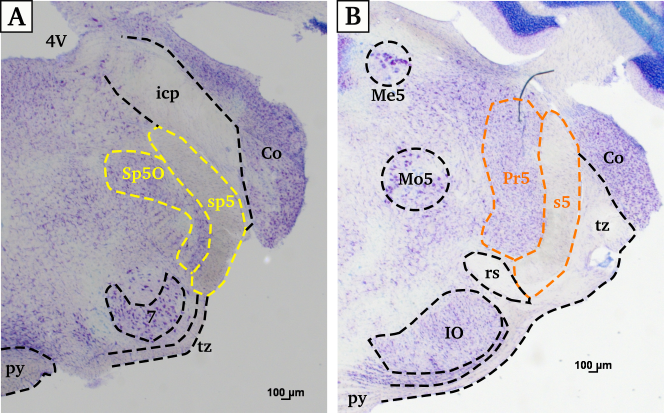
\includegraphics[width = \textwidth]
    {pictures/somatosensory/somato_kopf.png}
    \caption[Nucleus spinalis und Nucleus principalis des Trigeminus]{\textbf{Nucleus spinalis und Nucleus principalis des Trigeminus}\\
     \textbf{A} (N06\_4R): Der Nucleus spinalis oralis (Sp5O) liegt in der Medulla lateral auf der Höhe des Nucleus cochlearis (Co) und doral des Nucleus facialis (7). Des weiteren sieht man den spinalen Trigeminus (sp5) lateral des Nucleus. Weiter Strukturen sind: vierter Ventrikel (4V), inferior cerebelles Peduncle (icp), Pyramidenbahn (py), Trapezkörper (tz)
     \textbf{B} (N09\_3R): Der Nucleus principalis (Pr5) des Trigeminus liegt im Mesencephalon lateral-dorsal auf der Höhe der Inferioren Olive (IO). Die Axone zum Nucleus liegen im Trigeminus (s5). Weitere Strukturen sind: Nucleus cochlearis (Co), Nucleus mesencephalicus des Trigeminus (Me5), Nucleus motorius des Trigeminus (Mo5),  Pyramidenbahn (py), rubrospinaler Tract (rs), Trapezkörper (tz)}
    \label{fig:somato_Pr5}
\end{figure}

\subsubsection*{Nucleus mesencephalicus des Trigeminus}
Einige der Neurone die für die somatosensorische Reizweiterleitung aus dem Kopfbereich zuständig sind, haben ihre Zellkörper nicht im Ganglion Gasseri. Dazu gehören die Neurone die aus den Muskelspindeln kommen, und einige Neurone aus den Vibrissen und Neurone von den Zahnwurzeln. Die Zellkörper diese Neurone sind im Nucleus mesencephalicus des Trigeminus (Me5, Abb.~\ref{fig:somato_Pr5}) \index{Me5 !Nucleus mesencephalicus des Trigeminus}lokalisiert. Die Axone der Neuronen projizieren in den dorsomedialen Bereich des Nucleus principalis \index{Pr5 !Nucleus principalis} \textsuperscript{\cite[5]{heldmaier2003tierphysiologie}}.

\subsubsection*{Thalamus und Cortex}
Die Axone aus dem Nucleus principalis kreuzen die Mittellinie und stoßen zum medialen Lemniscus hinzu und ziehen in den Thalamus. Die Axone aus dem trigeminalen System ziehen in den medialen Part des Thalamus. Im Thalamus wird über synaptische Verschaltung die Information an die Nervenzellen der thalamocorticalen Verbindung zum primären somatosensorischen Cortex (S1) weiter gegeben. 
Wie schon in Kapitel \ref{subsubsec:S1} beschrieben ist S1 für die Verarbeitung der somatosensorischen Reize aus dem Körper verantwortlich. Bei Ratten kommt die meisten somatosensorischen Informationen aus den Vibrissen. Von jeder Vibrisse gehen um die 100 myelinisierte Nervenfasern ab. Über den Trigeminus werden die Informationen erst in den Nucleus principalis geleiten, von dort ziehen andere Neurone weiter in den Thalamus und von dort in den Cortex. Die Neuronen enden im Cortex in abgegrenzten Strukturen, sogenannten 'Barrel' (Abb.~\ref{fig:barrelcortex}B). Die Anzahl der 'Barrels' entsprechen den der Vibrissen und die 'Barrels' sind nach ihrem Aufbau benannt. In der Nissel-Färbung in Abbildung~\ref{fig:barrelcortex}C sieht man die Neurone dicht gepackt um weniger dichte Bereiche. Die Wände der Tonnen (eng.: barrels) sind die dicht gepackten Neurone und das Innere die weniger dicht gepackten Bereiche, daher der Name 'Barrels' \textsuperscript{\cite[8]{smith2008biology}}. 

\begin{figure}[H]
    \centering
    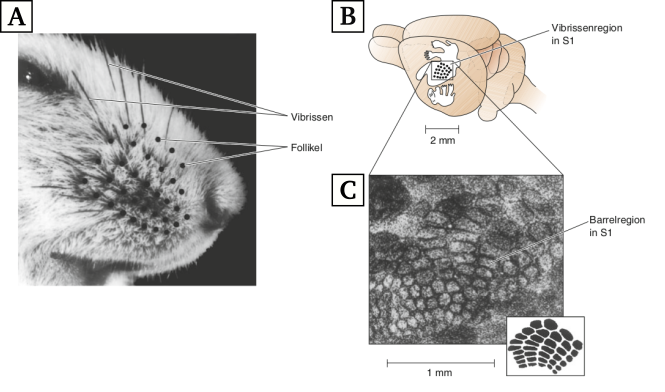
\includegraphics[width = \textwidth] {pictures/somatosensory/barrelcortex.png}
    \caption[Barrelcortex]{\textbf{Barrelcortex}\\
    \textbf{A}: Die Lage der Vibrissen am Beispiel einer Maus \textbf{B}: schematische Darstellung des primären somatosensorischen Cortex (S1) mit der Lage der 'Barrel' (englisch für Tonne, nach dem Aussehen der einzelnen cortikalen Areale jeder Vibrisse) in S1. Die 'Barrel' sind analog zur Lage der Vibrissen zueinander angeordnet. \textbf{C}: Barrelregion innerhalb von S1. Der Schnitt durch die 'Barrel' ist horizontal zum Cortex angelegt und mit Hilfe einer Nissel-Färbung angefärbt. Die Abbildung unten rechts, zeigt nochmal die Anordnung der Barrel in fünf Reihen wie auch in \textbf{A} zusehen ist.
    \textsuperscript{\cite{barrelcortex2008}}}
    \label{fig:barrelcortex}
\end{figure}

%%%%%%%%%%%%%%%%%%%%%%%%%%%%%%%%%%%%%%%%%%%%%%%%%%%%%%%%%%%%%%
%%%%%%%%%%%%%%%%%%%%%%%%%%%%%%%%%%%%%%%%%%%%%%%%%%%%%%%%%%%%%%

\newpage
\section{Spezielle sensorische Bahnen}
% verweis auf dieses Kapitel mit \ref{sec:spezsens}
\label{sec:spezsens}
Die speziellen sensorischen Bahnen umfassen unter anderem die Hörbahn, die Sehbahn und die Riechbahn, womit sich in diesem Kapitel vor allem beschäftigen wird. Diese drei speziellen sensorischen Bahnen spielen sowohl bei der Ratte als auch beim Schaf die zentrale Rolle. Es gibt weiter spezialisierte Sinne wie zum Beispiel den elektrischen Sinn bei Fischen, die beiden chemischen Sinne für Geruch und Geschmack und der Magnetsinn bei Zugvögeln \textsuperscript{\cite{smith2008biology}}. Diese werden nicht in dieser Zusammenfassung behandelt, spielen aber bei anderen Tierarten eine tragende Rolle und sollten aus diesem Grund hier kurz erwähnt werden.

\subsection{Hörbahn}

Das auditorische System ist für die Verarbeitung von Schallwellen, die über die Luft oder Wasser übertragen und vom System empfangen werden, zuständig. Vibrationen die über den Untergrund oder festes Substrat übertragen werden und mechanisch wahrgenommen werden, gehören zum Vibrationssinn der eng verwandt mit dem auditorischen Sinn ist.
\\
\noindent Dabei hat der auditorische Sinn zwei Aufgaben: zum einen die Detektion des Schalls und die Lokalisation der Schallwelle. Das Richtungshören ist nicht für alle Tiere möglich und ist auch bei den Tieren die dazu befähigt sind, nicht im gesamten Hörbereich gleich genau \textsuperscript{\cite[18]{penzlin2005tierphys}}.

\subsubsection*{Spiralganglion}
Die Funktion unserer Ohren ist die Energie eines akustischen Signals von der Außenwelt einzufangen und von einem mechanischen Signal in ein elektrisches Signal umzuwandeln. Diese Umwandlung findet an den inneren Haarsinneszellen in der Cochlea statt. Dort wird durch die Auslenkung der Haarbündel an den inneren Haarsinneszellen (eng.: inner hair cell, IHC) die Zelle depolarisiert oder hyperpolarisiert je nach Auslenkungsrichtung \textsuperscript{\cite[30]{kandel2013principles}}. Die Depolarisation der Haarzellen führt zur Öffnung spannungsgesteuerter Kalziumkanäle und dem damit verbundenen Einstrom von \ce{Ca^2+}. Durch den Einstrom des \ce{Ca^2+} wird der Neurotransmitter (wahrscheinlich Glutamat) freigesetzt und aktiviert die Spiralganglionzelle. Spiralganglionzellen sind bipolare Zellen, welche ihren Namen der spiralförmigen Struktur der Cochlea (Schneckenspindel) verdanken, der sie folgen\textsuperscript{\cite[11]{neurowissenschaften_baer}}. Sie formen einen Teil des achten Hirnnervs (CN~VIII), der auch Nervus vestibulocochlearis genannt wird. Ungefähr 30~000 Ganglionzellen im Hörnerv werden durch die inneren Haarzellen innerviert, das macht ungefähr 90\% des Nervs aus\textsuperscript{\cite[30]{kandel2013principles}}. 
Innere Haarzellen haben keinen efferente Eingang von höheren Hirnstrukturen. Anhand der Neuronenverteilung in der afferente Bahn wird die funktionale Bedeutung zwischen den inneren und äußeren Haarzellen erkennbar. Die afferenten Fasern ausgehend von den IHC sind myelinisiert (Typ I) und bilden 95\% der affrenten Fasern, wärend 5\% der Fasern, affrente unmyelinsierte Typ~II Fasern, von den äußeren Haarzellen kommen. Bei den inneren Haarzellen gibt dabei die Regel: Jedes Axon wird nur von eine Haarzelle innerviert, aber eine Haarzelle innerviert im Durchschnitt zehn Fasern.  \textsuperscript{\cite[30]{kandel2013principles}}.   
\\
\noindent Die affrenten Nervenfasern der IHC codieren die Stimulusfrequenz und die Intensität. Auf Grund der Beschaffenheit der Basilarmembran der Cochlea, werden die Frequenzen tonotopisch von hohen Frequenzen am ovalen Frenster bis zu tiefen Tönen am Helicotrema an der Basilarmembran entlang aufgeteilt\textsuperscript{\cite[22]{paxinos2014rat}}. Aufgrund ihrer Größe und Funktion sind die Type I Fasern, ausgehend von den inneren Haarzellen, sehr viel besser verstanden. Die Bahnen die die Informationen aus diesen Fasern nehmen werden im Folgenden als einzige thematisiert.

\begin{figure}[H]
    \centering
    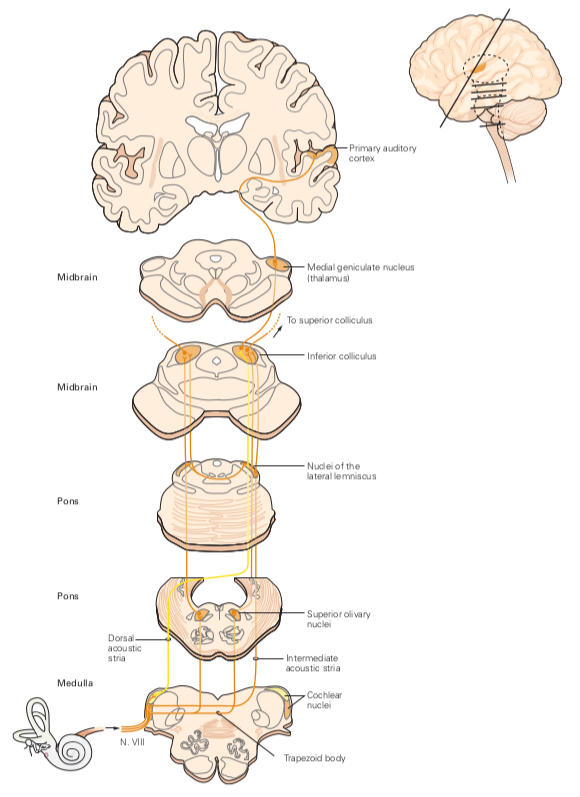
\includegraphics{pictures/auditory/hoerbahn_pathway.png}
    \caption[Hörbahn]{\textbf{Hörbahn} \\
    Die einzelnen Stationen der Hörbahn des Menschen von den Spiralganglionzellen in der Cochlea bis zum primären auditorischen Cortex anhand skizzierter Gehirnschnitte aus dem Kandel\textsuperscript{\cite[30]{kandel2013principles}} und einem Fließdiagramm}
    \label{fig:hoerbahn_pathway}
\end{figure}

\newpage
\noindent Efferente Fasern im Hörnerv innervieren die äußeren Haarzellen in der Cochlea, deren Aufgabe darin besteht die mechanische Auslenkung der Basilarmembran und der damit verbundenen Tektorialmembran zu verstärken oder zu unterdrücken. Infolgedessen kommt es zu einer verstärkten Selektivität und Sensibilität der Frequenzwahrnehmung\textsuperscript{\cite[22]{paxinos2014rat}}.

\subsubsection*{Nucleus cochlearis}

Die afferenten Ganglionzellen aus dem Hörnerv ziehen auf der Höhe der Medulla in den Hirnstamm und dort in das Kerngebiet den \textit{Nucleus cochlearis} (CN). Dieser befindet sich  lateral auf der Höhe der Medulla (Abb.~\ref{fig:hoerbahn_pathway}) und bekommt nur Input aus dem Hörnerv der ipsilateralen Seite. Der NC besteht aus dem dorsalen Nucleus cochlearis (DCN) und dem ventralen Nucleus cochlearis (VCN), welcher wiederum in den anteroventralen (AVCN) und den posteroventralen (PVCN) Nucleus unterteilt wird\textsuperscript{\cite[22]{paxinos2014rat}}. Bei Ratten liegt der ventrale Nucleus cochlearis flach mediolateral an der Medulla, während der dorsale Nucleus cochlearis sich um den 'restiform body'\textsuperscript{\cite[22]{paxinos2014rat}}.
\\ \noindent Die auditorischen Nervenfasern verzweigen sich im Nucleus cochlearis in die verschiedenen Teile des CNs (Abb.~\ref{fig:Nucleus_cochlearis}B). Jede Faser gabelt sich in einen aufsteigen Ast zum AVCN und einen absteigenden Ast zum PVCN und DCN und leitet die Informationen an verschiedene Neurone in den Teilbereichen weiter\textsuperscript{\cite[22]{paxinos2014rat}}. Die Neuronen im ventralen Nucleus cochlearis codieren verschieden Eigenschaften, je nach Zelltyp. Im Allgemeinen schärfen sie das Timing und die Information aus dem Klangspektrum. 
\\

\begin{figure}[H]
    \centering
    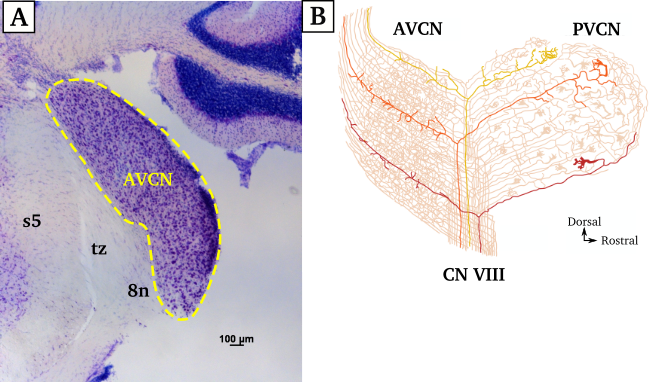
\includegraphics[width = \textwidth]{pictures/auditory/CN.png}
    \caption[Nucleus cochlearis]{\textbf{Nucleus cochlearis}\\
    \textbf{A}: Nissel-Färbung (N09\_1DL) der rechten Seite der Medulla. Es sind der anteroventrale Nucleus cochlearis (AVCN), der Trigeminus (s5), der Trapezkörper (tz) und der achte Hirnnerv (8n, Hörnerv) zu sehen. \textbf{B}: Verlauf der Nervenfasern aus dem achten Hirnnerv (CN VIII, 8n) im ventralen Nucleus cochlearis. Sowohl im anteroventralen (AVCN) als auch im posteroventralen (PVCN) Bereich des CNs werden die Fasern nach der Frequenz tonotopisch geordnet, von den tiefen Frequenzen (rot) ventral bis zu den hohen Frequenzen (gelb) im dorsalen Bereich. Abbildung B verändert nach Kandel \textsuperscript{\cite[31]{kandel2013principles}}}
    \label{fig:Nucleus_cochlearis}
\end{figure}

\newpage
Ein wesentlichen Teil spielt das Timing in der Weiterverarbeitung der Informationen in der oberen Olive, wohingegen die Verarbeitung des Klangspektrums in den ipsilateralen DCN, die ipsilaterale laterale obere Olive (LSO), den contralateralen ventralen Nucleus des lateralen Lemniscus und den contraleteralen Colliculus inferior projiziert wird\textsuperscript{\cite[31]{kandel2013principles}}. 
\\\\
\noindent Der dorsale Nucleus cochlearis bekommt einerseits direkten Input von den Neuronen aus dem Hörnerv, zum anderen indirekten Input aus dem ventralen CN. Der dorsale CN integriert akustische  und somatosensorische Informationen um die Richtung der Schallquelle zu bestimmen\textsuperscript{\cite[31]{kandel2013principles}}. 


\subsubsection*{Obere Olive}
Ein Großteil der Nervenzellen aus dem Nucleus cochlearis projizieren in die obere Olive. Die \textbf{obere Olive} (\textit{Nucleus olivaris superior}) ist für die Verarbeitung auditorischer Informationen wichtig und umfasst mehrere Kerngebiete. Innerhalb der Säugetiere variieren die Kerngebiete die unter dem Begriff obere Olive zusammengefasst werden. Drei Kerngebiete können bei fast allen Spezies gefunden werden: die \textbf{laterale obere Olive} (eng.: lateral superior olive, \textbf{LSO}), die \textbf{mediale obere Olive} (eng.: medial superior olive, \textbf{MSO}) und der \textbf{mediale Nucleus des Trapezkörpers} (eng.: medial nucleus of the trapezoid body, \textbf{MNTB}). Die LSO ist ein S-förmiges Kerngebiet im lateralen bereich der oberen Olive und ist durch ihre markante Struktur leicht zu erkennen (Abb.~\ref{fig:obere_Olive}). Die MSO liegt medial der LSO und ist bei Ratten ein kleineres Kerngebiet als beim Menschen. Der mediale Nucleus des Trapezkörpers (MNTB) befindet sich lateral in der oberen Olive\textsuperscript{\cite[29]{paxinos2014rat}}.

In Nagetieren, wie der Ratte, gibt es ein viertes, ausgeprägtes Kerngebiet, den \textbf{oberen paraoliven Nucleus} (eng.: superior paraolivary nucleus, \textbf{SPO}). Diese Kerngebiet befindet sich im dorsomedial Bereich der oberen Olive. Es bekommt die Informationen aus dem contralateralen Nucleus cochlearis und projiziert in den Colliculus inferior auf der ipsilateralen Seite\textsuperscript{\cite[29]{paxinos2014rat}}. Die SPO entschlüsselt besonders gut Muster in Tönen und Informationen in zeitlichen Mustern. Das spielt in der Wahrnehmung von Kommunikation ein Rolle, im Besonderen bei akustischen Schwebungen in Vokalisationen bei Tieren und Sprachsignalen\textsuperscript{\cite[29]{paxinos2014rat}}. 
\\\\

\noindent Die drei Hauptkerne der oberen Olive spielen eine wichtige Rolle in der Verarbeitung von Schall. Aufgrund der Beschaffenheit der Cochlea werden dort nur die einzelnen Frequenzen kodiert, wobei dadurch keine Informationen über die Richtung der Schallquelle kodiert werden. Das Richtungshören wird in der oberen Olive integriert, durch die Verarbeitung der Informationen aus beiden Ohren. Sie ist damit die erste Schaltstelle in der Hörbahn die Input von der ipsilateralen und der contralateralen Seite, aus den jeweiligen Nuclei cochlearis, bekommt.
\newpage
\textbf{Mediale obere Olive}

\noindent Die mediale obere Olive (\textbf{MSO}) ist tonotopisch arrangiert. Die tiefen Töne werden dorsal in der MSO verarbeitet, wohingegen hohe Frequenzen im ventralen Part verarbeitet werden. Der Anteil der tiefen Töne ist proportional über repräsentiert in der MSO. Aus diesem Grund ist die MSO in der Ratte (Abb.~\ref{fig:obere_Olive}) klein, da Ratten im hochfrequenten Bereich hören.

Die mediale obere Olive erhält excitatorischen Input aus den beiden Nuclei, wobei die lateralen Dendriten der MSO, die Informationen aus dem ipsilateralen Nucleus cochlearis erhalten und die medialen Dendriten aus dem contralateralen Nucleus\textsuperscript{\cite[29]{paxinos2014rat}}. Da die Neuronen aus den Nuclei nur auf eine bestimmt Phase des Tons feuern (eng.: \textbf{phase-locking}), kann mit Hilfe der interauralen Zeitdifferenz und dem 'coincidence detection model' die Richtung, aus der der Ton kam, bestimmt werden\textsuperscript{\cite[31]{kandel2013principles}}.

Die Axone der MSO projizieren in den \textbf{dorsalen Nucleus des lateralen Lemniscus} (\textbf{DLL}) und in den \textbf{Colliculus inferioris} (\textbf{IC})\textsuperscript{\cite[29]{paxinos2014rat}}.
\\

\begin{figure}[H]
    \centering
    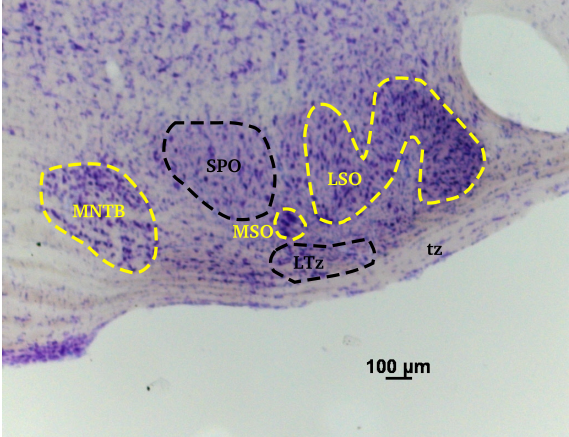
\includegraphics{pictures/auditory/obere_olive.png}
    \caption[Obere Olive]{\textbf{Obere Olive}\\
    Nissel-Färbung (N10\_1DL) der oberen Olive in der Pons. Mit den drei Hauptkernen mediale obere Olive (MSO), der lateralen oberen Olive (LSO) und dem medialen Nucleus des Trapezkörpers (MNTB) und dem für Nager speziellen oberen paraoliven Nucleus (SPO). Des weiteren liegt in der oberen Olive das Kerngebiet des lateralen Nucleus des Trapezkörpers (LTz) und der Trapezkörper (tz) selber, welcher die oberen Oliven beider Hirnhälften miteinander verbindet, befindet sich ventral des Komplex der oberen Olive.}
    \label{fig:obere_Olive}
\end{figure}

\newpage
\textbf{Laterale obere Olive}

\noindent Die laterale obere Olive (\textbf{LSO}) und der mediale Nucleus des Trapezkörpers (\textbf{MNTB}) zusammen, bilden eine Einheit, welche über die interaurale Intensitätsdifferenz das Richtungshören bei hohen Tönen, berechnet. 
 Die tonotopische Anordnung der LSO zieht sich entlang der S-Form von hohen Tönen medial bis zu tieferen Tönen lateral. Die LSO der Ratte ist im vergleich zum Menschen einiges größer, das Hängt unter anderem mit der Überrepresentation der hohen Töne in der lateralen oberen Olive zusammen und dem Hörbereich von Ratten.

Die LSO bekommt bilateralen Input. Der ventrale Nucleus cochlearis (VCN) der ipsilateralen Seite, leitet die Informationen excitatorisch an die LSO weiter. Vom contralateralen VCN werden die Informationen excitatorisch an den MNTB, der anderen Seite, über den Trapezkörper weiter gegeben. Von dort wird das Signal inhibitorisch an die LSO der selben Seite weiter geleitet.
Somit bekommen die Neuronen der LSO indirekten inhibitorischen Input aus dem contralateralen Nucleus cochlearis und excitatorischen Input aus dem ipsilateralen Nucleus cochlearis.

Die laterale obere Olive projiziert bilateral in den zentralen Nucleus des Colliculus inferior (\textbf{IC}), wobei auf die ipsilaterale Seite inhibitorisch projiziert wird und auf die contralaterale Seite excitatorisch.
Des weiteren projiziert ein Teil der Neuronen auch in den dorsalen Nucleus des lateralen Lemniscus (\textbf{DLL}) \textsuperscript{\cite[29]{paxinos2014rat}}.


\subsubsection*{Lateraler Lemniscus}

Die afferenten Nervenfasern aus der oberen Olive bilden den \textbf{Lemniscus lateralis} (\textbf{ll}) welcher über das Tegmentum pontis in den \textbf{Colliculus inferior} (\textbf{IC}) zieht und dort terminieren (Abb.~\ref{fig:lateraler_lemniscus}). Einige der Axone aus der oberen Olive terminieren in den \textbf{Nuclei des lateralen Lemniscus}. Des weiteren enden hier auch Nervenfasen die direkt aus den Nuclei cochlearis kommen \textsuperscript{\cite[10]{crossman2014neuroanatomy}}. 
Die Nuclei des lateralen Lemniscus unterteilen sich in den \textbf{dorsalen Nucleus des lateralen Lemniscus} (\textbf{DLL}) und den \textbf{ventralen Nucleus des lateralen Lemniscus} (\textbf{VLL}). Diese Unterteilung erfolgt anhand zweier funktional unterschiedlichen Systeme: die monoaurale Verarbeitung ventral und die binaurale Verarbeitung dorsal \textsuperscript{\cite[29]{paxinos2014rat}}. 
\\

\textbf{Ventraler Nucleus des lateralen Lemniscus}

Afferente Neuronen ziehen aus dem contralateralen ventralen Nucleus cochlearis (VCN) und dem ipsilateralen MNTB in den ventrale Nucleus des lateralen Lemniscus (\textbf{VLL}). Der VLL ist vorwiegend in der Verarbeitung von präzisen zeitlichen Informationen zuständig.
Es wird vermutet, dass die Zwischenstation in dem ventralen Nucleus als Relaisstation auf dem Weg zum Colliculus inferior funktioniert.
Der Nucleus ist aus isofrequenten Lamina aufgebaut und liegt in der Pons (Abb.~\ref{fig:lateraler_lemniscus}). Die Afferenzen zum Colliculus inferior sind ebenfalls tonotopisch arrangiert. Sie terminieren im zentralen Bereich des IC \textsuperscript{\cite[29]{paxinos2014rat}}.
\\

\textbf{Dorsaler Nucleus des lateralen Lemniscus}

Der dorsale Nucleus des lateralen Lemniscus (\textbf{DLL}) liegt oberhalb des ventralen Nucleus des lateralen Lemniscus in der Pons (Abb.~\ref{fig:lateraler_lemniscus}). Er bekommt bilateralen Input. Von der contralateralen Seite projizieren die Neuronen aus dem ventralen Nucleus cochlearis (VCN) und dem DLL, von der ipsilateralen Seite projizeren afferent Nervenfasern aus der MSO, SPO und dem VLL. Von beiden Seiten ziehen in den dorsalen Nucleus Afferenzen aus der lateralen oberen Olive (LSO).
Aufgrund der vielen Verbindungen zu tiefer liegenden Kernen wie der LSO und MSO spielt der dorsale Nucleus eine Rolle beim Richtungshören. Läsionen im DLL bewirken ein Defizit im Richtungshören und eine Ungenauigkeit in der räumlichen Hörschärfe. 
Der DLL projiziert über den lateralen Lemniscus in beide Colliculi inferior (IC) und über die Probst commisur in den gegenüberliegenden dorsalen Nucleus des lateralen Lemniscus
\textsuperscript{\cite[29]{paxinos2014rat}}.


\begin{figure}[H]
    \centering
    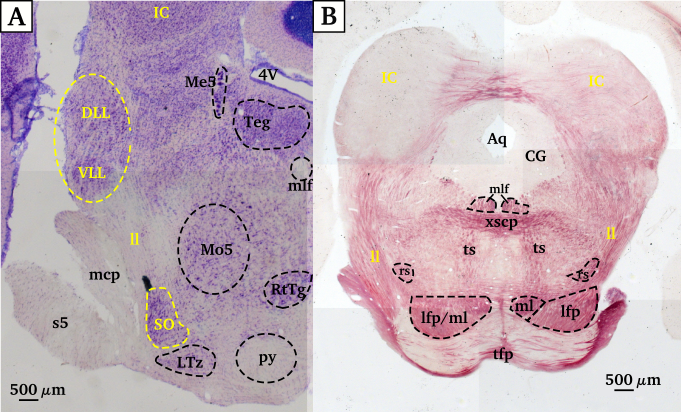
\includegraphics{pictures/auditory/lateral_lemniscus.png}
    \caption[Der Lateraler Lemniscus und seine Kerne]{\textbf{Der Lateraler Lemniscus und seine Kerne}\\
    Nissel-Färbung (N11\_4P) auf der Höhe der Pons, erkennbar am vierten Ventrikel (4V).
    Der laterale Lemniscus verbindet die obere Olive (SO) mit dem Colliculus inferior (IC). Einige der Verbindungen sind über d den dorsalen (DLL) oder den ventralen (VLL) Nucleus des lateralen Lemniscus zwischen geschaltet. 
    Des weiteren sind der Trigeminus (s5) und der Nucleus des mesencephalischen Tracts des Trigeminus (Me5) aus der Somatosensorik und der motorische Nucleus des Trigeminus (Mo5) aus der Motorik zu sehen. 
    Weitere Kerngebiete und Fasertracte sind: lateraler Nucleus des Trapezkörpers (LTz), mittlerer cerebellarer Penduncle (mcp), medialer Fasciculus longitudinalis (mlf), Pyramidenbahn (py), reticulotegmentaler Nucleus der Pons (RtTg), Tegmentum (Teg)
    }
    \label{fig:lateraler_lemniscus}
\end{figure}

\subsubsection*{Colliculus inferior und Corpus geniculatum mediale}

Die Fasern des lateralen Lemniscus ziehen in den \textbf{Colliculus inferior} (\textbf{IC}) und terminieren dort. Er liegt bei der Ratte sichtbar im dorsalen bereich auf dem Mittelhirn, caudal vom Colliculus superior und bildet mit diesem zusammen die Vierhügelplatte \textsuperscript{\cite[29]{paxinos2014rat}}. \textcolor{red}{verweis auf den colliculus im teil von jule} 
Der IC integriert nahezu die gesamten aus den tiefer liegenden auditorischen Kerngebieten des Hirnstamms. Das macht ihn zu einem großen Integrationszentrum für die verarbeitung des Richtungshören und auch für Tonhöhen \textsuperscript{\cite[29]{paxinos2014rat}}.

Vom Colliculus inferior aus geht die Hörbahn in den \textbf{medialen Kniehöcker} (\textit{Corpus geniculatum mediale}). Eine weitere Bahn führt direkt in den Colliculus superior (SC), welcher bei reflexiven Bewegungen zur Orientierung eine Rolle spielt. Desewgen nimmt man an dass, im SC eine auditorische Karte der Umgebung erstellt wird. Eulen sind bekannt für solche Karten die eine 3D Ansicht der Geräusche um sie herum sind. Zusammen mit Karten aus dem visuellen System und dem somatosensorischen System spielt der Colliculus superior eine entscheidende Rolle in motorischen Orientierung beim greifen nach Gegenständen \textsuperscript{\cite[31]{kandel2013principles}}.
\\
Der mediale Kniehöcker (\textbf{MG}) liegt auf der posterolateralen Seite des Thalamus. Es ist eine runde Erhebung lateral-ventral des Colliculus superior. Es ist das letzte Integrationszentrum in der auditorischen Hörbahn vor dem Cortex. Es bekommt Input aus dem Colliculus inferior (IC) über das \textit{Brachium colliculi inferioris} und absteigende Fasern aus dem auditorischen Cortex und dem reticularen Nucleus terminieren im MG. Afferente Nervenfasern aus dem medialen Kniehöcker ziehen ipsilateral in den auditorischen Cortex \textsuperscript{\cite[29]{paxinos2014rat}}. Der mediale Kniehöcker ist in drei Untereinheiten aufgeteilt: den ventralen, den dorsalen und den medialen Part. Der ventrale mediale Kniehöcker hat eine rein akustische Funktion, wohingegen der dorsale Part bei akustischer Aufmerksamkeit mitwirkt und der mediale Part bei multisensorischer Erregung und emotionalem akustischen Lernen eine Rolle spielt \textsuperscript{\cite[29]{paxinos2014rat}}.

\begin{figure}[H]
    \centering
    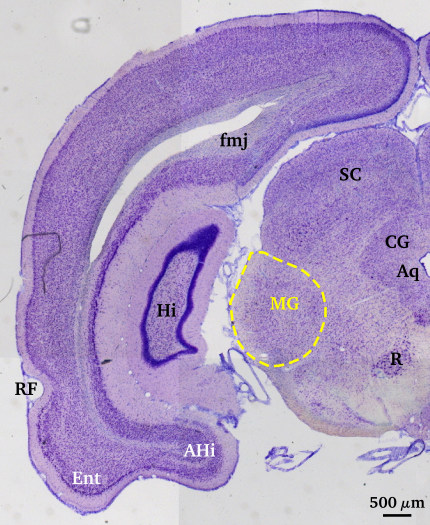
\includegraphics{pictures/auditory/MG.png}
    \caption[Corpus geniculatum mediale]{\textbf{Corpus geniculatum mediale}}
    \label{fig:MG}
\end{figure}

\subsubsection*{Primärer auditorischer Cortex}

\newpage
\subsection{Sehbahn}
\begin{itemize}
    \item eye
    \begin{itemize}
        \item kurzer überblick über die entwicklung des auges in der embryonal entwicklung retina aus dem diencephalon
        \item auf grund der evolutionären Entwicklunf ein "inverted" auge wesswegen die retina und die photorezeptoren nach innen weg vom licht gerichtet sind
        \item formung der retina: \cite{smith2008biology} p.287
        \item retinale zellen Stäbchen und zäpfchen und dann bipolar zellen und Ganglienzellen 
        \item vllt was zu den rezeptifen feldern
    \end{itemize}
    \item visual pathway
    \begin{itemize}
        \item 3 verschiedene wege ( vorlesung von oswald IN)
        \item wie heißen die von führen sie hin und wir konzentrieren uns auf einen zentralen und warum
    \end{itemize}
    \item optic nerve von der Retina zum Chiasma opticum
    \item Optic chiasm    \index{Chiasma opticum}
    \begin{itemize}
        \item Semidecussation  \index{Decussation!Semi-}
        \item ganglienzellen von der nasalen/medialen seite des auges kreuzen am optic chiasm auf die andere seite des gehirns wärend die laterale seite des auges auf der selben seite weiter projezieren
        ßitem keine verschaltung im optischen chiasma sondern nur eine kreuzung der ganglien zellen
        \item danach optic tract
    \end{itemize}
    \item Optic tract \index{optischer Trakt}
    \item LGN: nicht gestreift, hinterer Teil das Thalamus \index{Thalamus}, auf Höhe des superior colliculus \index{Colliculus superior, SC}
    \begin{itemize}
        \item lateral am Diencephalon \index{Diencephalon} vorbei
        \item posteriorer part des thalamus
        \item aufbau des LGN unterschied zwischen primaten (6 Schichten) und Ratten bzw. Schafen
        \item kurz was zur funktion der verschaltung auf der ebene ( vllt etwas zu den rezeptive fields aber dann auch schon auf der ebene der retina erwähnen)
        \item von LGN über die optic radiation (welche nicht in den schnitten sichtbar ist) ruaf in den neocortex und in V1 
    \end{itemize}
    \item Magnifikationsfaktor = Dichte der Zellen und wie sie verschaltet sind
    \\
\end{itemize}
\subsection{(Riechbahn)}
\begin{itemize}
    \item vom olfactorischen bulb über den olfactorischen trakt zu einerm der ältesten teile des neocortex zum Pyriformen lappen
    \item weitere neuronen führen dann zum thalamus un die weitern stränge dann in den orbitofrontal lobe \cite{smith2008biology} 
    \item eventuell Dopaminerge Bilder
\end{itemize}

\newpage
\section{Motorische Kerngebiete und Bahnen}
\subsection{Motorische Kerngebiete}
\subsection{Motorische Bahnen zum Hirnstamm}
\subsection{Motorische Bahnen zum Rückenmark}
\begin{itemize}
    \item laterales System: corticospinaler Trakt
    \item laterales System: rubrospinaler Trakt
    \item mediales System: reticulospinaler Trakt (medial,lateral)
    \item mediales System: vestibulospinaler Trakt
\end{itemize}
\subsection{Kleinhirn}
\begin{itemize}
    \item Vestibulocerebellum, Spinocerebellum, Corticocerebellum 
    \item Schichtung
    \item funktionelle Einheiten
    \item Schaltkreise
\end{itemize}
\subsection{(Motorik der Kopfmuskulatur)}
\subsection{(Motorik der Augen)}

\newpage
\section{Integrative Systeme}
\subsection{Limbisches System und Hippocampus}

\subsubsection*{Info zum Hippocampus}

\begin{itemize}

\item \textcolor{blue}{Hallo, ich hatte für meinen Teil was über den Hippocampus gesucht... Aber ich nehme nur die minimale Info rein, aber vielleicht kannst du was davon gebrauchen.. '' oder "" sind wörtliche Zitate. Die Quellen sollten irgendwo in den referneces hier zu finden sein :) LG Jule}

\item "Der Hippocampus (griechisch für„Seepferdchen“) hat für Lernen und Gedächtnis eine große Bedeutung" \cite[Kap.~7]{neurowissenschaften_baer}
	
\item 'The rat HF looks like a C-shaped structure (Fig. 2). Its long axis extends from the septal nuclei of the basal forebrain rostrodorsally, over and behind the diencephalon, into the caudoventral portion of the hemisphere, where HF abuts the rostrally adjacent amygdaloid complex' (Paxinos, Kap.~20)

\item 'Der Hippecampus liegt zum größten Teil im Schläfenlappen an der Medialwand des Seitenventrikeltmterhorns ( >- Abb. 9.16). Mit seinem rostralen Endstück bildet er dort eine tatzenähnliche Struktur (Pes hippocampi, >- Abb. 9.16, 1). Nach hinten oben reicht er, entsprechend der Rotationsbewegung der Hemisphären in der Embryonalentwickltmg, in einem Bogen bis zum kaudalen Ende des Balkens (Corpus callosurn). Von dort aus setzt er sich dann unterhalb des Balkens in die Faserstruktur
des Fomix fort( >- Abb. 9. 16, 4- 6). Der Fomix zieht in
einem Bogen über dem III. Ventrikel nach rostral m1d ventral weiter und endet in den Corpora mammillaria.' (trepel, Kap.~9)

\item Afferenzen:\\
'Afferenzen erhält der Hippocampus besonders zahlreich über den Tractus perforans von der medial des Hippecampus im Gyrus parabippocampalis (auch: Gyrus hippocampi) liegenden Area entorhinalis (auch: Regio entorhinalis). Über diese Region fließen dem Hippocampus u. a. modulierte sensorische lmpulse aus dem Neokortex und dem Rhinencephalon zu. Weiterhin erhält der Hippecampus afferente Fasern aus dem Thalamus, dem Gyrus cinguli, dem Corpus amygdaloideuro und über den Fornix aus dem Septum.' (trepel, Kap.~9)

\item Efferenzen:\\
'Nahezu alle Efferenzen des Hippocampus verlaufen im Fornix. Dieser gibt auf seinem Weg Faserzüge an das Septum, Corpus amygdaloideum sowie den Hypothalamus ab m1d endet mit dem Hauptteil der Fasern in den Corpora maillaria. Hierbei bildet sich der sog. Papez-Neuronenkreis ( >- Abb. 9.17): Der Hippecampus projiziert über den Fornix in die Corpora mammillaria.' (trepel, Kap.~9)

\item FUNKTION: 'Neben der sehr wichtigen Funktion für die Gedächtnisbildung wird der Hippocampus als Bestandteil des limbischen Systems mit endokrinen, vegetativen und emotionalen Vorgängen in Zusammenhang gebracht.' (trepel, Kap.~9)

\item 'der Hippocampus ist für den transfer von Gedächtnisinhalten vom kurzzeit- zum langzeitgedächtnis esentiell' \cite[Kap.~6]{storch2012lehrbuchzoo}

\item gehört zum lymbischen system \cite[Kap.~6]{storch2012lehrbuchzoo}

\item gehört zu den cortikalen arealen/gebieten  \cite[Kap.~6]{storch2012lehrbuchzoo}

\item the hippocampus is involved with aspects of memory storage (Kandel, Kap.1???)

\item 'The hippocampal formation includes the hippocampus, dentate gyrus, and subiculum. The hippocampus and associated cortical regions form the /oor of the temporal horn of the lateral ventricle (Figure 15–12). Together these structures are responsible for the formation of long-term memories about our daily experiences, so-called episodic memories, but are not the permanent storage site of these memories (see Chapter 65).Damage to the hippocampus interferes with people’s ability to form new memories but does not signi0-cantly impair the ability to retrieve old memories.' (Kandel, Kap.~15)

\item 'the hippocampus is thought to store memories temporarily through long-term synaptic plasticity. The hippocampus then transfers these memories to neocortex by inducing a replay in parietal, temporal, and frontal association cortex of activity patterns elicited by recent events.' (Kandel, Kap.~18)

\end{itemize}

\subsection{Basalganglien}

\newpage
\section{generelle Transmittersysteme (monoaminerge Systeme)}
\section{Quantitative Analyse generelle Transmittersysteme (am Beispiel der catecholaminergen Systeme)}
\subsection{Immunohistochemischer Nachweis catecholaminerger Neurone}
Der immunhistochemische Nachweis catecholaminerger Neurone lässt sich in sechs Einzelschritte unterteilen, diese sind in Material und Methoden auf S.xy zu finden.\newline
1. Quenching\newline
Um eine nicht-spezifische Hintergrundsfärbung durch endogene Peroxidasen zu vermeiden, wird im ersten Schritt durch die Zugabe von Wasserstoffperoxidase eine Reaktion unterbunden. \newline
2. Blocken\newline
Vor der Zugabe des ersten Antikörpers müssen zwei Schritte erfolgen: Zum einen sollen die Antikörper ausschließlich an die spezifischen Bindestellen binden, zum anderen muss den Antikörpern der Zugang zu intrazellulären Antigenen ermöglicht werden.
Um nicht-spezifische Protein-Protein-Interaktion zwischen Antikörpern und Proteinen im zu untersuchenden Gewebe zu unterbinden, werden blockende Poteine hinzuegegeben, die kompetetitv and die unspzifische Bindestelle binden. Hierbei binden Fc-Rezeptoren, welche auf Makrophagen und vielen anderen immunologischen Zellen des Gewebe zu finden sind and das Fc-Ende des Antikörpers und führen somit zur unspezifischen Bindung. 
Um die Antigene des zu untersuchenden Gewebes zugänglich zu machen, muss die Zellmembran vorerst mit Detergenzien bahendelt werden, die die Doppellipidschicht durch Verseifung auflockern - die Permabilisierung.\newline
3. Primärer Antikörper\newline
Der primäre Antikörper besitzt eine Fc-Region, die artspezifisch an unsere Host Bindestelle binder und eine Fab-Region, die an das Epitop des Antigens (Tyrosin-Hydroxylase) bindet.\newline
4. Sekundärer Antikörper\newline
Nun bindet die Fc-Region des ersten Antikörpers and die Fab-Region des zweiten Antikörpers. Der zweite Antikörper ist biotyniliert. \newline
5. Der ABC-Complex\newline
Nachdem das Avidin die biotylinielierte Meerrettich-Peroxidase gebunden hat, kann es nun auch an das biotynilierte Ende des sekundären Antikörpers binden. Dieser Schritt dient der Amplifizerung des Signals.\newline
6. DAB Reaktion\newline
Wasserstoffperoxid bindet and die Meerrettich-Peroxidase und oxidiert das DAB, welches reduziert und nun als bräunliches Edukt vorliegt und somit indirekt die erfolgreiche Bindung and das Antigen sichtbar macht.\newline

\subsection{Lage und Größe der Kerngebiete und Projectionsareale}
\subsection{Dopaminerges und Noradrenegres System}
\begin{itemize}
    \item Incertohypothalamic/nigrostriatal System (Dopamin)
    \item Tuberohypophysial System (Dopamin)
    \item Locus coeruleus (Noradrenalin)
\end{itemize}
\subsection{Größenvergleich der Neurone in \textit{substantia nigra} und \textit{locus coeruleus}}



%%%%%%%%%%%%%%%%%%%%%%%%%%%%%%%%%%%%%%%%%%%%%%%%%%%%%%%%%%5%%
% Bibliography

\newpage
\bibliographystyle{unsrt}
\bibliography{references}

%%%%%%%%%%%%%%%%%%%%%%%%%%%%%%%%%%%%%%%%%%%%%%%%%%%%%%%%%%%%%
% Index
\printindex

2n - II optic nerve
3V - 3. Ventrikel\\
3n - III oculomotor nerve\\
4V - 4. Ventrikel\\
5n - V Trigeminus\\
6n - VI nervus abducens\\
\\
Aq - Aquaeductus cerebri\\
Amy - Amygdala\\
ACx - Archicortex\\
\\
CCx - cingulärer Cortex\\
Cu - Nucleus caudatus\\
CPu - Caudoputamen (Striatum)\\
cc - corpus callosum / Balken\\
ChP - choroid plexus\\
Cx - cerebraler Cortex\\
cp - cerebellar peduncle\\
CS - cortical Spine / cortikales Rückenmark\\
Cb - Cerebellum\\
\\
Epi - Epiphyse\\
EO - epithelium olfactorium\\
\\
f - Fornix\\
fi - Fimbria\\
\\
Hi - Hippocampus\\
Hyp - Hypophyse\\
\\
IC - Inferior colliculus\\
ICj - Islands of Calleja\\
\\
LGN - lat. genuculate nuc.\\
lot - lat. olfactory tract\\
LV - lateraler Ventrikel
\\
Med - Medulla\\
MB - mammillary body\\
\\
NCx - Neocortex\\
\\
OB - olfactory bulb / Riechkolben\\
ox - chiasma opticum\\
ot - olfactory tract / olfaktorischer Trakt\\
\\
Pon - Pons\\
PM - Pia mater\\
\\
RF - rhinal fissure\\
\\
SC - Superior colliculus / Colliculus inferior\\
\\
Th - Thalamus\\
Teg - Tegmentum\\
tz - trapezoid body / Trapezkörper\\
TC - Truncus cerebri / Hirnstamm\\
Tu - olfactory tubercle\\
\\
Ve - Velum\\
\\



\end{document}


